%!TEX program = xelatex

% safe参数解决与\!在内的多个冲突
% \sups命令可能被重定义,xeCJK放在tipa后
\RequirePackage[safe]{tipa}
\documentclass[a4paper, zihao=-4, linespread=1]{ctexrep}
  \xeCJKsetup{CJKmath=true}
  \renewcommand{\CTEXthechapter}{\thechapter}


% 中文支持
% \iffalse与\fi可以实现“多行注释”
\iffalse
\usepackage[slantfont,boldfont]{xeCJK}
	\setCJKmainfont[BoldFont=SimHei,ItalicFont=KaiTi]{SimSun}
	\setCJKmathfont{STXinwei}
\usepackage{indentfirst}
\fi
\setCJKmathfont{KaiTi}
\newCJKfontfamily[zhxinwei]\xinwei{STXinwei}

% 数学环境
\usepackage{amsmath}
  \newcommand{\ue}{\mathrm{e}}
  \newcommand{\ud}{\mathop{}\negthinspace\mathrm{d}}
\usepackage{amssymb}
\usepackage{mathrsfs} % 线性代数字体
    % overline的替代命令
\newcommand{\closure}[2][3]{{}\mkern#1mu\overline{\mkern-#1mu#2}}
\usepackage{yhmath} % 左下-右上省略号
\usepackage{mathtools} % dcases环境
\usepackage{amsthm} % 定理环境
  \theoremstyle{definition}\newtheorem{laws}{Law}[section]
  \theoremstyle{plain}\newtheorem{ju}[laws]{Jury}
  \theoremstyle{remark}\newtheorem*{marg}{Margaret}
\usepackage{esint} % 多重积分,需放在amsmath后

% 下划线宏包
\usepackage{ulem}
% LaTeX符号宏包
\usepackage{hologo}
	\newcommand{\xelatex}{\Hologo{XeLaTeX}}
	\newcommand{\bibtex}{\Hologo{BibTeX}}
% 其他符号
\usepackage{wasysym}
% 带箱小页
\usepackage{boxedminipage}
% 绘图
\usepackage{tikz}
	\usetikzlibrary{calc}
	\newcommand{\tikzline}[1]{{#1\tikz{\draw[#1,line width=9](0,0)--(0.5,0);}}, }

% 奇怪的小定义
\newcommand{\dpar}{\\ \mbox{}}	% 空两行
\newcommand{\qd}[1]{{\bfseries{#1}}}	% 强调
\newcommand{\co}[1]{{\bfseries{#1}}}   % Style of concept
\newcommand{\RED}[1]{{\color{cyan}{#1}}}
\newcommand{\cmmd}[1]{\fbox{\texttt{\char92{}#1}}}
\newcommand{\charef}[1]{第\ref{#1}章}
\newcommand{\secref}[1]{第\ref{#1}节}
\newcommand{\pref}[1]{第\pageref{#1}页}
\newcommand{\fref}[1]{图\ref{#1}}
\newcommand{\tref}[1]{表\ref{#1}}

% 编号列表宏包,并自定义了三个列表
\usepackage[inline]{enumitem}
	\setlist[enumerate]{label=\arabic* - ,font=\bfseries,itemsep=0pt}
	\setlist[itemize]{label=$\bullet$,font=\bfseries,leftmargin=\parindent}
	\setlist[description]{font=\bfseries\uline}

\newenvironment{fead}{\setlength{\parskip}{0pt}
	\begin{description}[font=\bfseries\uline,labelindent=\parindent]
		\setlength{\itemsep}{0pt}\setlength{\parsep}{0pt}\setlength{\parskip}{0pt}}
	{\end{description}}
% 带宽度的
\newenvironment{para}{\setlength{\parskip}{0pt}
	\begin{description}[font=\bfseries\ttfamily]
		\setlength{\itemsep}{0pt}\setlength{\parsep}{0pt}\setlength{\parskip}{0pt}}
	{\end{description}}
\newenvironment{feae}{\setlength{\parskip}{0pt}
	\begin{enumerate}[font=\bfseries,labelindent=0pt]}
	{\end{enumerate}}
\newenvironment{feai}{\setlength{\parskip}{0pt}
	\begin{itemize}[font=\bfseries]
		\setlength{\itemsep}{0pt}\setlength{\parsep}{0pt}\setlength{\parskip}{0pt}}
	{\end{itemize}}
\newenvironment{inlinee}
{\begin{enumerate*}[label=(\arabic*), font=\rmfamily, before=\unskip{:},itemjoin={{;}},itemjoin*={{,以及:}}]}
	{\end{enumerate*}。}

% 目录和章节样式
\usepackage{titlesec}
\usepackage{titletoc}   % 用于目录

\titlecontents{chapter}[1.5em]{}{\contentslabel{1.5em}}{\hspace*{-2em}}{\hfill\contentspage}
\titlecontents{section}[3.3em]{}{\contentslabel{1.8em}}
	{\hspace*{-2.3em}}{\titlerule*[8pt]{$\cdot$}\contentspage}
\titlecontents*{subsection}[2.5em]{\small}{\thecontentslabel{} }{}{, \thecontentspage}[;\qquad][.]
% 章节样式
\setcounter{secnumdepth}{3} % 一直到subsubsection
\newcommand{\chaformat}[1]{%
	\parbox[b]{.5\textwidth}{\hfill\bfseries #1}%
	\quad\rule[-12pt]{2pt}{70pt}\quad
	{\fontsize{60}{60}\selectfont\thechapter}}
\titleformat{\chapter}[block]{\hfill\LARGE\sffamily}{}{0pt}{\chaformat}[\vspace{2.5pc}\large
	\startcontents\printcontents{}{1}{\setcounter{tocdepth}{2}\songti}]
%\titleclass{\section}{top}
%\titleformat{\section}{\Large\bfseries}{\thesection}{0.5em}{}
\titleformat*{\section}{\centering\Large\bfseries}
\titleformat{\subsubsection}[hang]{\bfseries\large}{\rule{1.5ex}{1.5ex}}{0.5em}{}
% 扩展章节
\newcommand{\starsec}{\noindent\fbox{\S\textit{注意:本章节是一个扩展阅读章节。}}
	\\ \mbox{}}

\renewcommand{\contentsname}{目录}
	\renewcommand{\tablename}{表}
	\renewcommand\arraystretch{1.2}	% 表格行距
	\renewcommand{\figurename}{图}
% 设置不需要浮动体的表格和图像标题
\setlength{\abovecaptionskip}{5pt}
\setlength{\belowcaptionskip}{3pt}
\makeatletter
\newcommand\figcaption{\def\@captype{figure}\caption}
\newcommand\tabcaption{\def\@captype{table}\caption}
\makeatother
% 图表
\usepackage{array,multirow}
  \setlength\extrarowheight{2pt} % 行高增加
\usepackage{longtable}
\usepackage{graphicx}
  \graphicspath{{./tikz/}}
% 页面修正宏包
\usepackage{geometry}
\geometry{top = 1in}

% 代码环境
\usepackage{listings}
% Avoid copy line numbers of the listing code (Invalid for SumatraPDF Reader)
\usepackage{accsupp}
	\newcommand{\emptyaccsupp}[1]{\BeginAccSupp{ActualText={}}#1\EndAccSupp{}}
% Color
\usepackage{xcolor}
  \newcommand{\scol}[1]{\colorbox{#1}{\rule{0em}{1ex}}\,#1}
	\definecolor{commentcolor}{RGB}{85,139,78}
	\definecolor{numbercolor}{RGB}{166,206,168}
	\definecolor{stringcolor}{RGB}{206,145,108}
	\definecolor{keywordcolor}{RGB}{34,34,250}
	\definecolor{backcolor}{RGB}{220,220,220}
	\definecolor{packagecolor}{RGB}{0,128,0}
	\definecolor{envicolor}{RGB}{185,70,15}
% LaTeX Code Style
\lstset{language=[LaTeX]TeX,
		basicstyle=\small\ttfamily,
		commentstyle=\color{commentcolor},
		keywordstyle=\color{keywordcolor},
		stringstyle=\color{stringcolor},
		showstringspaces=false,
		% Package/Tikz-Lib Using
		classoffset=0,
		morekeywords={begin,end,usetikzlibrary},
		keywordstyle=\color{keywordcolor},
		classoffset=1,
		morekeywords={article,report,book,
			xeCJK,tikz,
			calc},
		keywordstyle=\color{packagecolor},
		classoffset=2,
		morekeywords={document,tikzpicture},
		keywordstyle=\color{envicolor},
		% Line Number Style
		numbers=left,
		numberstyle=\tiny\emptyaccsupp,
		stepnumber=1,
		% Frame and Background Color
		frame=single,
		framerule=0pt,
		backgroundcolor=\color{backcolor},
		% Spaces
		% belowskip=\medskipamount,
		emptylines=1,
		escapeinside=``}

\lstnewenvironment{latex}[1]{\lstset{#1}}{}
\newcommand{\latexline}[1]{{\lstinline[language=TeX,basicstyle=\small\ttfamily]{#1}}}

% Tikz Code
\lstdefinelanguage{tikzlang}{
	classoffset=0, % 蓝色的keyword
	morekeywords={begin,end,newcommand,
		draw,node,coordinate,tikzstyle,foreach},
	keywordstyle=\color{keywordcolor},
	classoffset=1, % 棕色的其他关键字
	morekeywords={tikzpicture,grid,at,
		thick,thin,very,ultra,
		red,green,yellow,blue,cyan,magenta,black,
		    gray,darkgray,lightgray,brown,lime,
		    olive,orange,pink,purple,teal,violet,white},
	keywordstyle=\color{envicolor},
	morecomment=[l]{\%},
	morecomment=[s]{/*}{*/},
	morestring=[b]',
	% Escape
	escapeinside=``
}
\lstnewenvironment{tikzcode}[1]{\lstset{language=tikzlang,basicstyle=\small\ttfamily,
		breaklines=true,%backgroundcolor=\color{white},
		linewidth=0.7\linewidth,#1}}{}

% 附录
\usepackage{appendix}
\renewcommand{\appendixname}{App.}

% 行号
\usepackage{lineno}

% 代码输入环境
\usepackage{verbatim,xcolor}
\newbox\savedlines
\newtoks\savedtokens
\makeatletter
\def\codeshow{%
\global\savedtokens={}%
\def\verbatim@processline{%
{\setbox0=\hbox{\the\verbatim@line}%
\hsize=\wd0
\the\verbatim@line\par}%
\global\savedtokens=\expandafter{\the\expandafter\savedtokens\the\verbatim@line^^J}}%
\@tempswatrue
\setbox0=\vbox\bgroup\parskip=0pt\topsep=0pt\partopsep=0pt
\verbatim}
\def\endcodeshow{\endverbatim%
\unskip\setbox0=\lastbox\egroup
\global\setbox\savedlines=\box0
\addvspace{1em}\par\noindent%
\colorbox{lightgray}{%
\begin{minipage}{.55\textwidth}{\usebox\savedlines}\end{minipage}}%
\hfill\fbox{\parbox{.40\textwidth}%
{\scantokens\expandafter{\the\savedtokens\unskip\endinput}}}%
\par\addvspace{1em}}
\makeatother

\usepackage{booktabs}

\bibliographystyle{plain}
\renewcommand{\bibname}{参考文献}
\usepackage[square,super,sort&compress]{natbib}

% 引用
\usepackage{hyperref}
\hypersetup{colorlinks, bookmarksopen = true, bookmarksnumbered = true, pdftitle=LaTeX-cn, pdfauthor=K.L Wu, pdfstartview=FitH}

\title{简单粗暴\LaTeX\ }
\author{K.L Wu\\
  {\kaishu 本手册是\href{https://github.com/wklchris/Note-by-LaTeX}{wklchris-GitHub}的\LaTeX{}-cn项目}
}
\date{当前版本号:v1.6.3\\
  最后更新于:\today}

\begin{document}

\maketitle

\setlength{\lineskiplimit}{0pt}
\tableofcontents
\setlength{\lineskiplimit}{3pt}

\chapter{序}

\noindent{\Huge\xinwei 第一稿序}\dpar\dpar

其实在之前我是有一稿手册的,开始撰写的日期大概在2015年4月。但是自己觉得写得太烂,因此索性推倒重写了这一版。这一版的主要特征是:
\begin{feae}
  \item 我希望能够吸引初学者快速上手,解决手头的问题。因此去掉了枯燥的讲解和无穷无尽的宏包用法介绍,直接使用实例;
  \item 力求突出实用性。当然,也会提点一些可以深入学习的内容,读者可以自行查阅,或者阅读本手册中的扩展阅读章节(即带星号*的章节)。
  \item 本手册使用的编辑器为\TeX\ Studio,而非之前的商业软件WinEdt. 这使得学习\LaTeX\ 的门槛更低。当然了,你有权使用任何编辑器。
\end{feae}

手册主体分为六大部分\cite{LHY2013latex,lamport1994latex,frank2004latex,partl2016,Casteleyn2016tikz}:
\begin{fead}
\item[写给读者*] 介绍\LaTeX\ 背景、优缺点、适用情形。
\item[基础] 包括标点、缩进、距离、章节、字体、颜色、注释、引用、封面、目录、列表、图表、页面等详细内容。
\item[数学排版] 包括数学符号、公式、编号等内容。
\item[进阶] 主要是自定义命令,帮助你更高效、更简洁地书写你的文档。
\item[\tikzz\  绘图*] 附加章节,需要读者取消注释后重编译。
\item[附录] 帮助你快速查找一些你想要的东西。
\end{fead}

由于工作全部由我一人完成,限于视野,难免存在错漏之处。恳请读者指正。如遇到的手册中无法解决的问题,欢迎向我提出。推荐书目可参考本手册附录。

最后,还要感谢在\LaTeX\ 学习中为我解答疑惑的同学,特别是来自\LaTeX\ 度吧的吧友;本手册中许多的解决方案都是由他们提供的。我谨在此记录。

\vfill

\begin{flushright}
Mail: wklchris@hotmail.com\dpar

Chris Wu

September 17, 2016 于Davis, CA
\end{flushright}
\clearpage
\noindent{\Huge\xinwei 更新日志:}\dpar\dpar

版本号以 $x.y.z$ 的形式公示。当$z=0$时,为决定正式 release 的版本。

v1.6.0 更新 --- 2017年6月15日:

v1.6.1 更新 --- 2017年8月9日;

v1.6.2 更新 --- 2017年10月5-15日。

v1.6.3 更新 --- 2018年3月22日。\dpar

以下内容中,未以括号注明的项是在v1.6.0中更新的。

\begin{feai}
\item 重要更新:
  \begin{feai}
  \item \textbf{\sout{\tikzz\  相关的内容停止更新}。原因是现有的其他软件绘图功能强大,导出为 pdf 格式的矢量图后也易于调用;\tikzz\  相比之下学习成本过高。}\textcolor{red}{\textbf{笔者又决定重启\tikzz\ 章节}}。(v1.6.3)
  \item \textbf{重新添加了 \tikzz\  章节} —— 不过仍是之前弃笔时的版本,预计将于 v1.7 更新。
  \item \textbf{增加了加快\xelatex 调用字体速度的方式}。参考“中文支持与CJK字体”一节\texttt{fc-cache}相关内容。(v1.6.1)
  \end{feai}
\item 字体更换:思源宋体。
\item 编辑了 Head.tex 文件,使之更易阅读。
\item [添加]宏包\pkg{animate}:在 PDF 中展示动态图。(v1.6.1)
\item [添加]宏包\pkg{tocbibind}:
  \begin{feai}
  \item 将目录本身编入目录项。
  \item 将参考文献章节编号、编入目录项。
  \item 将索引章节编号、编入目录项。
  \end{feai}
\item [更新]宏包\pkg{dcolumn},更详细说明了如何在表格中使用小数点对齐。(v1.6.2)
\item [更新]宏包\pkg{fancyvbr}:更详细说明了抄录环境\envi{BVerbatim},如何提供居中支持。(v1.6.2)
\item [更新]宏包\pkg{xeCJK}:
  \begin{feai}
  \item 参数 CJKspace。该功能在新版宏包中已修复。
  \item 命令 \latexline{setCJKmainfont},可指定字体文件名。
  \end{feai}
\item 数学内容:
  \begin{feai}
  \item [添加]宏包\pkg{extarrows}:长等号命令。
  \item [添加]命令\latexline{numberthis},用于给多行公式中的某行编号。(v1.6.2)
  \item [添加]命令\latexline{allowdisplaybreaks},用于支持多行公式环境换页。
  \end{feai}
\item 拆分了文档,并修改了“文档拆分”一节的内容。(v1.6.3)
\item 修复了一些错别字与无效的文档内跳转链接。
\end{feai}

\mbox{}

更早版本的更新细节,请到\href{https://github.com/wklchris/Note-by-LaTeX/releases}{Project Release Webpage}浏览。

% Main Contents

%!TEX root = ../LaTeX-cn.tex
\chapter{\mbox{写给读者}*}

我见过许多朋友初试\LaTeX ,他们都感到非常不能理解。主要有以下几个疑问:
\begin{feae}
\item “我平常使用MS Word,似乎也能完成科技排版工作,为什么我还需要\LaTeX ?”\hfill \textit{——见“为什么需要\LaTeX ?”一节。}
\item “\LaTeX 看上去不像是排版工具,更像是编程语言。我讨厌用写代码一样的方式来写文章。”\hfill \textit{——文本文件使你更专注于内容而不是排版细节。}
\item “\LaTeX 能生成doc文件吗?我平时上交作业/提交汇报时难道使用不便修改pdf文件么?”\hfill \textit{——见“\LaTeX 生成的文件格式?”一节。}
\end{feae}

本章希望能解决读者的这些疑问,让读者对于\LaTeX 有基础的了解,再决定是否需要学习。当然,如果你是被迫进入了\LaTeX 这个坑,你也可以阅读本章,或许本章能让你喜欢上\LaTeX 呢。

\section{什么是\LaTeX ?}
先讲\TeX (读音类似于“泰赫”)。

\TeX 是Knuth\footnote{Donald Ervin Knuth(高德纳,1938--),现代计算机科学的先驱者,斯坦福大学计算机系的终身荣誉教授,图灵奖和冯诺依曼奖得主,\TeX 和 \hologo{METAFONT} 的发明人。同时也是业内经久不衰的著作\emph{The Art of Computer Programming}的作者。}研发的免费、开源的排版系统,其初衷是为了“改变排版界糟糕的排版技术”,并用于排版他的著作《计算机程序设计艺术》。

\TeX 对于读者来说应该是底层的内容,如果你有兴趣,可以阅读Knuth著的\emph{The \TeX book},这本书是学习\TeX 最权威的材料,没有之一。在本手册的参考文献中也给出了其他\TeX 学习的资料。\dpar

再讲\LaTeX (读音类似于“拉泰赫”)。

\LaTeX 是基于\TeX 的宏\footnote{“宏(Macro)”是一个计算机概念,指用单个命令或操作完成一系列底层命令或操作的组合。}集,其作者是Dr.~Lamport\footnote{Leslie Lamport(1941--),美国计算机科学家,图灵奖和冯诺依曼奖得主。};其姓氏开头两个字母La与底层排版系统\TeX 相结合,就组成了名称\LaTeX 。\LaTeX 在\TeX 基础上定义了众多的宏命令,使得用户可以更方便地进行排版。本手册的参考文献中就有他的作品。

\LaTeX 现在的版本是\LaTeXe ,意思是2.x版而没到3.0版。错位排版的字母E和字母A暗示了它是排版系统。在无法这样输出的场合,请写作LaTeX和LaTeX~2e。

\section{\TeX 与\LaTeX 的优缺点}
\TeX 的优点:\qd{稳定、精确、美观}。底层的\TeX 系统已经很多年没有进行大的变动了,因为它注重\uline{稳定};\TeX 系统可以让你把排版内容通过数字参数的方式写到任意的位置,量化的参数意味着\uline{精确};\TeX 底层的空距调整机制,以及对于数学公式近乎完美的支持,则确保了排版效果的\uline{美观}。

\LaTeX 是基于\TeX 的,自然不会抛弃上述\TeX 的优点。具体包括:
\begin{feai}
\item 排版出来就是印刷品。专业而美观。
\item 易用、全面的数学排版支持,无出其右。
\item 撰写文档时不会被文档排版细节干扰精力。你可以使用之前自定义的模板,或者方便地在文字组织完毕后调整你的模板,以轻松达到满意的效果。
\item 复杂的排版功能支持,比如图表目录、索引、参考文献管理、高度自定义的目录样式、双栏甚至多栏排版。
\item 丰富的功能以及易寻的帮助文档。众多的\LaTeX 宏包赋予了\LaTeX 强大的扩展功能,它们都自带文档供你学习。
\item 源文件是\RED{文本文件}\footnote{文本文件的另一个优点是易于进行版本控制,比如利用git. 你可以方便地比较你相比上次修改了什么内容,也可以方便地恢复到之前某个时刻的版本。}。你可以在任何设备、任何文本编辑器中书写文档内容,无须担心复制时格式的变化;最后粘贴到同一个tex文件中编译即可。
\item 跨平台,免费,开源。
\end{feai}

那缺点呢?我认为主要有:
\begin{feai}
\item 入门门槛高。想要熟练地使用\LaTeX 并轻松地编写有自己的风格的文档,不是一两天就能够达到的。
\item 并非“所见即所得”,需要编译才能看到效果。编译查错有时令人恼火。
\item 完善一个自己的模板可能需要很长的时间。尽管\LaTeX 原生定义的模板能够满足绝大多数场合的需要。
\item 排版长表格有些复杂。但作为补充,在表格内插入数学公式是非常简单的。
\end{feai}

\section{为什么需要\LaTeX ?}
你可能基于以下原因学习\LaTeX :
\begin{feae}
\item 你的投稿对象要求你使用\LaTeX 排版,而不是MS Word——这种情况对没听说过\LaTeX 的你来说,真是糟糕透了。
\item 你需要在多个设备上撰写同一份文档。但你发现把内容在多个文档间复制粘贴时,格式总是会出现问题。
\item 你受够了MS Word自带的公式编辑器,或者你觉得购买的插件MathType的效果也不尽如人意。但你经常需要排版公式。
\item 你想参加某个科学竞赛,比如MCM,然后你发现你的朋友用的一个叫\LaTeX 的东西似乎还不错。
\item 你想出版一本书,或者投稿你的作品——结果他们告知你如果你使用\LaTeX 而不是MS Word攥写原稿件,他们会更快地把作品印刷出来。
\item 呃……也许,你只是喜欢学习新事物?
\end{feae}

对于科研工作者或者在校研究生,我认为\LaTeX 是非常优秀的工具。如果你是本科生,或者更年轻的群体,你也可以先学习\LaTeX ,因为到了研究生和工作中,学习的时间可能就非常有限了。

\section{MS Word难道不优秀吗?}
我想说的是,\qd{MS Word当然是优秀的软件}。但是它与\LaTeX 的定位不同,所以它们分别适用于不同场合。前者注重简单组织内容,后者注重排版效果。

在\uline{排版书籍、科学文档}方面,\LaTeX 非常专业、美观,公式支持性极佳,几乎所有参数你都可以量化调整。如果你想\uline{高度自定义一份文件},比如拥有特殊几何、颜色元素,且易于更改模板的简历,\LaTeX 可以完全独当一面。在这些这方面,MS Word是无法匹敌\LaTeX 的。

但是如果你只是为了生成\uline{非正式的文档},比如1--2页的作业稿;或者只是一份\uline{易于别人修改的非科学稿件},比如一份需要同事修改的演讲稿……那你无须使用\LaTeX 。这些方面,\LaTeX 无疑是比不上MS Word的。

\section{\LaTeX 生成的文件格式?}
一般广为使用的是pdf,以及dvi的格式。\LaTeX 无法生成doc或者docx扩展名文件,因为那是属于MS的商用格式,两者的工作机理也完全不同。

所以很遗憾,如果你身处一个要求你“必须提交docx”的环境中,那么\LaTeX 对你并不是一个好选择。但我想指出的是,这是稳定、优秀的pdf格式没有得到你身处环境认可的遗憾——pdf也可以方便地添加批注,并在不同设备的显示上有更好的稳定性。
%!TEX root = ../LaTeX-cn.tex
\chapter{\LaTeX{}基础}
\section{第一份文稿}

编辑器的配置大概是需要讲解一下的,毕竟对于初学者来说是很头疼的事情。本手册就以\TeX\ Studio为例进行配置。首先你应该安装一个\TeX{} Live,它是完全免费的,网址:\url{http://tug.org/texlive/}.

虽然它体积较大,但是却是最一劳永逸、最不需要花时间去配置的方法,同时它大概也是功能支持最强的\LaTeX\ 发行版。

打开\TeX\ Studio后,选择选项$\rightarrow$ 设置\TeX\ Studio $\rightarrow$ 构建$\rightarrow$ 默认编译器,选择\xelatex{}. 这主要是基于中文文档编译的考虑,同时\xelatex 也能很好地编译英文文档。我建议始终使用它作为默认编译器。\dpar

之后你可以在窗口输入一篇小文档,并保存为tex扩展名的文件进行测试:
\begin{latex}
\documentclass{ctexart}
\begin{document}
    Hello, world!
    你好,世界!
\end{document}
\end{latex}

点击编译按钮生成,F7查看。生成的pdf在你的tex文件保存目录中。具体各行的含义我们会在后文介绍。

\section{认识\LaTeX}
\subsection{命令与环境}
\LaTeX\ 中的\co{命令}通常是由一个反斜杠加上命令名称,再加上花括号内的参数构成的(有的命令不带参数,例如:\latexline{TeX})。
\begin{latex}
\documentclass{ctexart}
\end{latex}

如果有一些选项是备选的,那么通常会在花括号前用方括号标出。比如:
\begin{latex}
\documentclass[a4paper]{ctexart}
\end{latex}

还有一种重要指令叫做\co{环境}。它被定义于控制命令\latexline{begin\{environment\}} 和\latexline{end\{environment\}}间的内容。比如:
\begin{latex}
\begin{document}
...内容...
\end{document}
\end{latex}

环境如果有备选参数,只需要写在\latexline{begin[...]\{name\}}这里就行。

注意:不带花括号的命令后面如果想打印空格,请加上\RED{一对内部为空的花括号}再键入空格。否则空格会被忽略。例如:\verb+\LaTeX{} Studio+.

\subsection{保留字符}

\LaTeX\ 中有许多字符有着特殊的含义,在你生成文档时不会直接打印。例如每个命令的第一个字符:反斜杠。单独输入一个反斜杠在你的行文中不会有任何帮助,甚至可能产生错误。\LaTeX\ 中的保留字符有:
\begin{center}
\texttt{\# \$ \% \^ \& \_ \{ \} \char92}
\end{center}

它们的作用分别是:
\begin{para}
\item[\#{}:] 自定义命令时,用于标明参数序号。
\item[\${}:] 数学环境命令符。
\item[\%{}:] 注释符。在其后的该行命令都会视为注释。如果在回车前输入这个命令,可以防止行末\LaTeX\ 插入一些奇怪的空白符。
\item[\^{}:] 数学环境中的上标命令符。
\item[\&{}:] 表格环境中的跳列符。
\item[\_{}:] 数学环境中的下标命令符。
\item[\{与\}:] 花括号用于标记命令的必选参数,或者标记某一部分命令成为一个整体。
\item[\char92{}:] 反斜杠用于开始各种\LaTeX\ 命令。
\end{para}

以上除了反斜杠外,均能用前加反斜杠的形式输出。即你只需要键入:
\begin{center}
\verb|\# \$ \% \^ \& \_ \{ \}|
\end{center}

唯独反斜杠的输出比较头痛,你可以尝试:
\begin{codeshow}
$\backslash$ \textbackslash
\texttt{\char92}
\end{codeshow}

其中命令\latexline{char[num]}是一个特殊的命令,使用环境需要是tt字体环境,用于输出ASCII码对应的字符;92对应的即反斜杠。你也可以用\latexline{char`}后加字符的方式输出你想输出的命令,但需要包裹在\latexline{texttt}或者\latexline{ttfamily}内。如果想输出的字符是保留字符,需要再加一个反斜杠。
\begin{verbatim}
\texttt{\char`~} % 输出一个波浪线
\texttt{\char`\\} % 输出保留字反斜杠
\texttt{\char`@} % 实际上可直接输入@
\end{verbatim}

另外需要说明的是,上例提及的波浪线{\texttt{\~}}用来输出一个禁止在该处断行的空格,也不能够直接输出。尝试:
\begin{codeshow}
a $\sim$ b
a\~ b
a\~{} b
a\textasciitilde b
\end{codeshow}

\subsection{导言区}
任何一份\LaTeX{}文档都应当包含以下结构:
\begin{latex}
\documentclass[`\itshape options`]{doc-class}
\begin{document}
    ...
\end{document}
\end{latex}

其中,在语句\latexline{begin\{document\}}之前的内容称为\co{导言区}。导言区可以留空,以可以进行一些文档的准备操作。你可以粗浅地理解为:\RED{导言区即模板定义}。\dpar

文档类的参数doc-class和可选选项{\textit{options}}有\tref{tab:documentclass}取值:
\begin{table}[!htb]
    \centering
	\caption{文档类和选项}
	\label{tab:documentclass}
	\begin{tabular}{p{5em} @{\ -\ } p{24em}}
		\hline
		\multicolumn{2}{l}{\bfseries doc-class文档类\footnotemark} \\
		\hline
		article   & 科学期刊,演示文稿,短报告,邀请函。\\
		proc      & 基于article的会议论文集。\\
		report    & 多章节的长报告、博士论文、短篇书。\\
		book      & 书籍。\\
		slides    & 幻灯片,使用了大号Scans Serif字体。\\
		\hline
		\multicolumn{2}{l}{\bfseries\itshape options} \\
		\hline
		字体     & 默认10pt,可选11pt和12pt.\\
		页面方向 & 默认竖向portrait,可选横向landscape。\\
		纸张尺寸 & 默认letterpaper,可选用a4paper, b5paper等。\\
		分栏     & 默认onecolumn,还有twocolumn。\\
		双面打印 & 有oneside/twoside两个选项,用于排版奇偶页。article/report默认单面。\\
		章节分页 & 有openright/openany两个选项,决定是在奇数页开启新页或是任意页开启新页。注意article是没有chapter(``章'')命令的,默认任意页。\\
		公式对齐 & 默认居中,可改为左对齐fleqn;默认编号居右,可改为左对齐leqno。\\
		草稿选项 & 默认final,可改为draft,使行溢出的部分显示为黑块。\\
		\hline
	\end{tabular}
\end{table}

在本文中,多数的文档类提及的均为report/book类。如果有article类将会特别指明。其余的文档类不予说明。本手册排版即使用了report类。\dpar

在导言区最常见的是\co{宏包}的加载工作,命令形如:\latexline{usepackage\{package\}}。通俗地讲,宏包是指一系列已经制作好的功能``模块'',在你需要使用一些原生\LaTeX\ 不带有的功能时,只需要调用这些宏包就可以了。比如本文的代码就是利用\pkg{listings}宏包实现的。

宏包的具体使用将参在各部分内容说明中进行讲解。如果你想学习一个宏包的使用,按Win+R组合键呼出运行对话框,输入texdoc加上宏包名称即可打开宏包帮助pdf文档。例如:\verb|texdoc xeCJK|。

\footnotetext{此外还有\pkg{beamer}宏包定义的beamer文档类,常用于创建幻灯片。}

\subsection{错误的排查}
\label{subsec:debug}
在编辑器界面上,下方的日志是显示编译过程的地方。在你编译通过后,会出现这样的字样:
\begin{feai}
	\item {\qd{Errors错误}}:严重的错误。一般地,编译若通过了,该项是零。
	\item {\qd{Warnings警告}}:一些不影响生成文档的瑕疵。
	\item {\qd{Bad Boxes坏箱}\footnote{Box是\LaTeX{}中的一个特殊概念,具体将在\hyperref[sec:box]{这里}进行讲解。}}:指排版中出现的长度问题,比如长度超出(Overfull)等。后面的Badness表示错误的严重程度,程度越高数值越大。这类问题需要检查,排除Badness高的选项。
\end{feai}

你可以向上翻阅日志记录(即.log文件),来找到Warning开头的记录,或者Overfull/ Underfull开头的记录。这些记录会指出你的问题出在哪一行(比如line 1-2) 或者在pdf的哪一页(比如active [12]。注意,这个12表示计数器计数页码,而不是文件打印出来的真实页数)。此外你还需要了解:
\begin{feai}
	\item 值得指出的是,由于\LaTeX{}的编译原理(第一次生成aux文件,第二次再引用它),目录想要合理显示\qd{需要连续编译两次}。在连续编译两次后,你会发现一些Warnings会在第二次编译后消失。在\TeX\ Studio中,你可以只单击一次“构建并查看”,它会检测到文章的变化并自动决定是否需要编译两次。
	\item 对于大型文档,寻找行号十分痛苦。你需要学会合理地拆分tex文件,参阅\secref{sec:include}的内容。
\end{feai}

这里也推荐宏包\pkg{syntonly},在导言区加入它支持的\latexline{syntaxonly}命令,会只排查语法错误而不生成任何文档,这可以使你更快地编译。不过它似乎不太稳定,例如本文档可以正常编译,但是使用该命令时则会出错。

\subsection{文件输出}
\LaTeX{}的输出一般推荐pdf格式,由\LaTeX\ 直接生成dvi的方法并不推荐。

你在tex文档的文件夹下可能看到的其他文件类型:
\begin{tabbing}
	.sty{\hspace{2em}}\=宏包文件\\
	.cls	\> 文档类文件。\\
	.aux    \> 用于储存交叉引用信息的文件。因此,在更新交叉引用(公式编号、\\
	\> 大纲级别)后,需要编译两次才能正常显示。\\
	.log    \> 日志。记录上次编译的信息。\\
	.toc    \> 目录文件。\\
	.lof    \> 图形目录。\\
	.lot    \> 表格目录。\\
	.idx    \> 如果文档中包含索引,该文件用于储存索引信息。\\
	.ind	\> 索引记录文件。\\
	.ilg	\> 索引日志文件。\\
	.bib	\> \bibtex 参考文献数据文件。\\
	.bbl	\> \bibtex 生成的参考文献记录。\\
	.bst	\> \bibtex 模板。\\
	.blg	\> \bibtex 日志。\\
	.out	\> \texttt{hyperref}宏包生成的pdf书签记录。
\end{tabbing}

有时\LaTeX\ 的编译出现异常,你需要删除文件夹下除了tex以外的文件再编译。此外,在某些独占程序打开了以上的文件时(比如用Acrobat打开了pdf),编译可能出现错误。请在编译时确保关闭这些独占程序。

\section{标点与强调}
英文符号$|<>+=$一般用于数学环境中,如果在文本中使用,请在它们两侧加上“\$”。如果你在\LaTeX\ 中直接输入大于、小于号而不把它们放在数学环境中,它们并不会被正确地打印。你应该使用\latexline{textgreater}, \latexline{textless}命令。

在部分科技文章中,中文的句号可能使用全角圆点“.”\footnote{这个标点是 U+FF0E,称为 FULLWIDTH FULL STOP。},而不是平常的“。”,也不是正常的英文句点“.”。这个符号很难正常输入;你可以先输入正常句点,最后再替换。

\subsection{引号}
英文单引号并不使用两个\verb|'|符号组合。左单引号是重音符\verb|`|(键盘上数字1左侧),而右单引号是常用的引号符。英文中,\RED{左双引号就是连续两个重音符}。

英文下的引号嵌套需要借助\latexline{thinspace}命令分隔,比如:
\begin{codeshow}[listing side text, listing options={escapeinside=++}]
``\thinspace`Max' is here.''
\end{codeshow}
% 这里临时修改了listing的escapeinside, 使得这一行代码也可以被 codeshow 环境表示, 也使得行文风格更加统一
中文下的单引号和双引号你可以用中文输入法直接输入。

\subsection{破折、省略号与短横}
英文的短横分为三种:
\begin{feai}
\item 连字符:输入一个短横:\verb|-|,效果如daughter-in-law
\item 数字起止符:输入两个短横:\verb|--|,效果如:page 1--2
\item 破折号:输入三个短横:\verb|---|,效果如:Listen---I'm serious.
\end{feai}

中文的破折号你也许可以直接使用日常的输入方式。中文的省略号同样。但是注意,英文的省略号使用\latexline{ldots}这个命令而不是三个句点。

\subsection{强调:粗与斜}
\LaTeX\ 中专门有个叫做\latexline{emph\{text\}}的命令,可以强调文本。对于通常的西文文本,上述命令的作用就是斜体。如果你对一段已经这样转换为斜体的文本再使用这个命令,它就会取消斜体,而成为正体。

西文中一般采用上述的斜体强调方式而不是粗体,例如在说明书名的时候可能就会使用以上命令。关于字体的更多内容参考\hyperref[sec:font]{字体}这一节。

\subsection{下划线与删除线}
\LaTeX\ 原生提供的\latexline{underline}命令简直烂的可以,建议你使用\pkg{ulem}宏包下的\texttt{uline}命令代替,它还支持换行文本。\pkg{ulem}宏包还提供了一些实用命令:

\begin{codeshow}
\uline{下划线} \\
\uuline{双下划线} \\
\dashuline{虚下划线} \\
\dotuline{点下划线} \\
\uwave{波浪线} \\
\sout{删除线} \\
\xout{斜删除线}
\end{codeshow}

需要注意的是,\pkg{ulem}宏包重定义了\latexline{emph}命令,\RED{使得原来的加斜强调变成了下划线、原来的两次强调就取消强调变成了两次强调就双下划线}。通过宏包的normalem选项可以取消这个更改:\verb|\usepackage[normalem]{ulem}|。

\subsection{其他}
角度符号或者温度符号需要借助数学模式\verb|$...$|输入:

\begin{codeshow}
$30\,^{\circ}$三角形 \\
$37\,^{\circ}\mathrm{C}$
\end{codeshow}

欧元符可能需要用到\pkg{textcomp}宏包支持的\latexline{texteuro}命令。

其次是千位分隔位,比如\verb|1\,000\,000|。如果你不想它在中间断行就在外侧再加上一个\latexline{mbox}命令:\latexline{mbox\{1\char`\\,000\char`\\,000\}}。也可以使用\pkg{numprint}或者\pkg{siunitx}宏包中的相关命令。

再次是注音符号,比如\^o,也常用于拼音声调,参考\hyperref[app:phonetic]{注音符号表}部分的附录内容。如果你想输入音标,请使用tipa宏包\footnote{tipa会重定义\latexline{!}命令,因此请使用\latexline{negthinspace}代替;或在\pkg{xeCJK}与\pkg{amsmath}宏包前加载,并使用safe选项。具体可以参见本手册的 Head.tex 文件。},同样参考附录A。

最后,介绍\pkg{hologo}宏包,它可以输出许多\TeX\ 家族标志。其实\LaTeX\ 原生自带了\latexline{LaTeX}, \latexline{TeX}等命令。而hologo宏包支持的命令有:

\begin{codeshow}
% 大写H表示符号的首字母也大写
\hologo{XeLaTeX} \Hologo{BibTeX}
\end{codeshow}

\section{格式控制}
首先了解一下\hologo{LaTeX}的长度单位:
\begin{fead}
  \item[pt] point,磅。\label{sec:length}
  \item[pc] pica。1pc=12pt,四号字大小
  \item[in] inch,英寸。1in=72.27pt
  \item[bp] bigpoint,大点。1bp=$\frac{1}{72}$in
  \item[cm] centimeter,厘米。1cm=$\frac{1}{2.54}$in
  \item[mm] millimeter,毫米。1mm=$\frac{1}{10}$cm
  \item[sp] scaled point。\Hologo{TeX} 的基本长度单位,1sp=$\frac{1}{65536}$pt
  \item[em] 当前字号下,大写字母M的宽度。
  \item[ex] 当前字号下,小写字母x的高度。
\end{fead}

然后是几个常用的长度宏,更多的长度宏使用会在表格、分栏等章节提到。
\begin{latex}
\textwidth % 页面上文字的总宽度,即页宽减去两侧边距。
\linewidth % 当前行允许的行宽。
\end{latex}

有时候你可以使用可变长度,比如“\texttt{5pt plus 3pt minus 2pt}”,表示一个能收缩到3pt也能伸长到8pt的长度。直接使用倍数也是允许的,例如:1.5\latexline{parindent}等。

我们通常使用\latexline{hspace}和\latexline{vspace}这两个命令控制特殊的空格,具体的使用方法参考\hyperref[sec:hvspace]{水平和竖直距离}这一节。

\subsection{空格、换行与分段}
在\LaTeX\ 中,多个空格会被视为一个,多个换行也会被视为一个。如果你想要禁止\LaTeX\ 在某个空格处的换行,将空格用\texttt{\char126}命令替代即可,比如“\texttt{Fig.\char126 8}”。

通常的换行方法非常简单:\hologo{LaTeX}会自动转行,然后在每一段的末尾,只需要输入两个回车即可完成分段。如果需要一个空白段落(实质是一个空白行),先输入两个回车,再输入\latexline{mbox\{\}},最后再输入两个回车即可。你可以用\latexline{par}来产生一个带缩进的新段。

在下划线一节的例子中已经给出了强制换行的方式,即两个反斜:\latexline{\char`\\}. 不过这样做的缺点在于下一行段首缩进会消失,这个命令也的确一般\RED{不用于}正文换行;\textbf{正文中想要换行,请直接使用两个回车}。

段落之间的距离由\latexline{parskip}控制,默认\texttt{0pt plus 1pt}. 
\begin{latex}
\setlength{\parskip}{0pt}
\end{latex}

宏包\pkg{lettrine}能够产生首字下沉的效果:
\begin{codeshow}
\lettrine{T}{his} is an example. Hope you like this package, and enjoy your \LaTeX\ trip!
\end{codeshow}

\subsection{分页}
用\latexline{newpage}命令开始新的一页。

用\latexline{clearpage}命令清空浮动体队列\footnote{参见\hyperref[sec:float]{浮动体}这一节的内容。},并开始新的一页。

用\latexline{cleardoublepage}命令清空浮动体队列,并在偶数页上开始新的一页。

注意:以上命令都是基于\latexline{vfill}的。如果要连续新开两页,请在中间加上一个空的箱子(\latexline{mbox\{\}}),如\latexline{newpage\char`\\mbox\{\}\char`\\newpage}。

\subsection{缩进、对齐与行距}
英文的段首不需要缩进。但是对中文而言,段首缩进需要借助\pkg{indentfirst}宏包来完成。你可能还需要使用\latexline{setlength{\char`\\parindent}\{2em\}}这样的命令来设置缩进距离。如果在句首强制取消缩进,你可以在段首使用\latexline{noindent}命令。

\LaTeX\ 默认使用两端对齐的排版方式。你也可以使用\envi{flushleft}, \envi{flushright}, \envi{center}这三种环境来构造居左、居中、居右三种效果。特殊的\latexline{centering}命令常常用在环境内部(或者一对花括号内部),以实现居中的效果。但请尽量用\envi{center}环境代替这个老旧的命令。类似的命令还有\latexline{raggedleft}来实现居右,\latexline{raggedright}来实现居左。更多的空格控制请参考\hyperref[sec:hvspace]{这一节}。

插入制表位、悬挂缩进、行距等复杂的调整参考\hyperref[sec:hvspace]{这部分}的内容。

\section{字体与颜色}
\label{sec:font}
这一节只讨论行文中字体使用。数学环境内字体使用请参考\hyperref[sec:mathfont]{这一节}的内容。

\subsection{字族、字系与字形}
字体(typeface)的概念非常令人恼火,在电子化时代,基本上也都以字体(font)作为替代的称呼。宋体、黑体、楷体,这属于\co{字族};对应到西文就是罗马体、等宽体等。加粗、加斜属于\co{字系和字形}。五号、小四属于\co{字号}。这三者大概可以并称\co{字体}\footnote{本文中的字族、字系等称呼难以找到统一标准,可能并不是准确的名称。}。

\subsection{中西文“斜体”}
首先需要明确一点:\RED{汉字没有加斜体}。平常我们看到的加斜汉字,通常是几何变换得到的结果,非常的粗糙,并不严格满足排版要求;而真正的字形是需要精细的设计的。同时,汉字字体里面也很少有加粗体的设计。

西文一般设有加斜,但是这与“斜体”并不是同一回事。加斜是指某种字族的Italy字系;而斜体,是指Slant字族。在行文中表强调时使用的是前者;在Microsoft Word等软件中看到的倾斜的字母\textit{I},也代表前者。

\subsection{原生字体命令}
\LaTeX\ 提供了基本的字体命令,包括\tref{tab:fontcommand}中显示的内容。
\begin{table}[!ht]
\centering
\caption{\LaTeX\ 字体命令表}
\label{tab:fontcommand}
\begin{tabular}{p{3em}<{\centering} @{\ -\quad} l @{\quad-\quad} p{18em}}
\hline
字族 & \latexline{rmfamily} & 把字体置为{\rmfamily Roman}罗马字族。\\
     & \latexline{sffamily} & 把字体置为{\sffamily Sans Serif}无衬线字族。\\
     & \latexline{ttfamily} & 把字体置为{\ttfamily Typewriter}等宽字族。\\
\hline
字系 & \latexline{bfseries} & 粗体{\bfseries BoldSeries}字系属性。\\
     & \latexline{mdseries} & 中粗体{\mdseries MiddleSeries}字系属性。\\
\hline
字形 & \latexline{upshape}  & 竖直{\upshape Upright}字形。 \\
     & \latexline{slshape}  & 斜体{\slshape Slant}字形。 \\
     & \latexline{itshape}  & 强调体{\itshape Italic}字形。 \\
     & \latexline{scshape}  & 小号大写体{\scshape Scap}字形。 \\
\hline
\multicolumn{3}{l}{\ttfamily 如果临时改变字体,使用\latexline{textrm}, \latexline{textbf}这类命令。}\\
\hline
\end{tabular}
\end{table}

字族、字系、字形三种命令是互相独立的,可以任意组合使用。但这种复合字体的效果有时候无法达到(因为没有对应的设计),比如\latexline{scshape}字形和\latexline{bfseries}字系。\LaTeX\ 会针对这种情况给出警告,但仍可以编译,只是效果会不同于预期。

如果在文中多次使用某种字体变换,可以将其自定义成一个命令。这时请使用text系列的命令而不要使用family, series或shape系列的命令。否则需要多加一组花括号防止“泄露”。以下二者等价:
\begin{latex}
\newcommand{\concept}[1]{\textbf{#1}}
\newcommand{\concept}[1]{{\bfseries #1}}
\end{latex}

更多自定义命令的语法请参考\hyperref[sec:newcommand]{这一节}。

然后就是字号的命令。行文会有一个默认的“标准”字号,比如你在documentclass的选项中设置的12pt(如果你设置了的话)。\LaTeX\ 给出了一系列“相对字号命令”,列出如\tref{tab:fontsize}。此外,\pkg{ctex}宏包的\latexline{zihao}命令,参数$0$--$8$以及$-0$--$-8$表示初号到八号、小初到小八\footnote{日常使用的小四为12pt,五号为10.5pt。}。
\begin{table}[!ht]
\centering
\caption{相对字号命令表}
\label{tab:fontsize}
\begin{tabular}{|l|*{3}{l|}}
\hline
命令         & 10pt & 11pt & 12pt \\
\hline
\latexline{tiny}         & 5pt  & 6py  & 6pt  \\
\latexline{scriptsize}   & 7pt  & 8pt  & 8pt  \\
\latexline{footnotesize} & 8pt  & 9pt  & 10pt \\
\latexline{small}        & 9pt  & 10pt & 11pt \\
\latexline{normalsize}   & 10pt & 11pt & 12pt \\
\latexline{large}        & 12pt & 12pt & 14pt \\
\latexline{Large}        & 14pt & 14pt & 17pt \\
\latexline{LARGE}        & 17pt & 17pt & 20pt \\
\latexline{huge}         & 20pt & 20pt & 25pt \\
\latexline{Huge}         & 25pt & 25pt & 25pt \\
\hline
\end{tabular}
\end{table}

如果你想设置特殊的字号,使用:
\begin{latex}
\fontsize{font-size}{line-height}{\selectfont <text>}
\end{latex}

其中font-size填数字,单位pt;一般而言,line-height填\latexline{baselineskip}\footnote{这个命令的意义是行与行之间的基线间距(即行距),默认是1.2倍文字高。}。

默认全文的字体使用\latexline{rmfamily}族的字体。你可以通过重定义的方式更改它,使\latexline{rmfamily, \char`\\textrm}命令都指向新的字体。甚至把默认字体改为sf/tt字族。
\begin{latex}
\renewcommand{\rmdefault}{`\textit{font-name}`}
% 默认字体改为sf字族,也可用\ttdefault
\renewcommand{\familydefault}{\sfdefault}
\renewcommand{\sfdefault}{`\textit{font-name}`}
% 如果你排版CJK文档,还需要更改CJK的默认字体
\renewcommand{\CJKfamilydefault}{\CJKsfdefault}
\end{latex}

\subsection{西文字体}
\LaTeX\ 预包含字体如\tref{tab:alphafont}(参考\url{http://www.tug.dk/FontCatalogue/}):
\begin{table}[!hbt]
\centering
\caption{部分\LaTeX\ 西文字体}
\label{tab:alphafont}
\begin{tabular}{>{\ttfamily}ll}
\hline
命令 & \texttt{字体名} \\
\hline
cmr & \myfont{cmr}{Computer Modern Roman} (默认) \\
lmr & \myfont{lmr}{Latin Modern Roman} \\
pbk & \myfont{pbk}{Bookman} \\
ppl & \myfont{ppl}{Palatino} \\
lmss & \myfont{lmss}{Latin Modern Roman Serif} \\
phv & \myfont{phv}{Helvetica} \\
lmtt & \myfont{lmtt}{Latin Modern} \\
\hline
\end{tabular}
\end{table}

以上可以这样使用:
\begin{latex}
\newcommand{\myfont}[2]{{\fontfamily{#1}\selectfont #2}}
\renewcommand{\rmdefault}{ptm} % 可更改默认字体,同理可改sfdefault等
% 以上在导言区定义。在正文中:
Let's change font to \myfont{ppl}{Palatino}!
\end{latex}

在\xelatex 编译下,一般使用\pkg{fontspec}宏包来选择\textbf{本地安装}的字体。注意:该宏包可能会明显增加编译所需的时间。
\begin{latex}
\usepackage{fontspec}
  \newfontfamily{\lucida}{Lucida Calligraphy}
  \lucida{This is Lucida Calligraphy}
\end{latex}

该宏包的\latexline{setmathrm/sf/tt}与\latexline{setboldmathrm}命令可以支持你更改数学环境中调用的字体。

另外,你也可以通过简单地加载\pkg{txtfont}宏包,设置西文字体为Roman体,且同时会为你设置好数学字体。其他的简单字体宏包还有\pkg{cmbright},提供的CM Bright与\TeX\ 默认字体Computer Modern协调的不错;以及提供Palatino字体的\pkg{pxfonts}。另外的字体宏包在此不再介绍。

\subsection{中文支持与CJK字体}
中文方面,\pkg{ctex}宏包直接定义了新的中文文档类ctexart, ctexrep与ctexbook,以及ctexbeamer幻灯文档类。例如本手册\texttt{Head.tex}中:
\begin{latex}
\documentclass[a4paper, zihao=-4, linespread=1]{ctexrep}
  \renewcommand{\CTEXthechapter}{\thechapter}
\end{latex}

以上设置字号为小四,行距因子为1(故行距为$1\times 1.2=1.2$倍,其中1.2是\LaTeX\ 默认的基线间距)。而a4paper选项继承与原生文档类report,可见ctex文档类还是很好地保留了原生文档类的特征。\RED{值得注意的是,ctex文档类会用\texttt{\char92 CTEX}开头的计数器命令代替原有的},除非你使用\texttt{scheme=plain}来让ctex文档类\uline{仅支持中文而不做任何文档细节更改}。具体的使用参考ctex宏包文档。

\pkg{ctex}宏包支持以下字体命令:
\begin{center}
\tabcaption{\texttt{ctex}宏包支持的字体命令}
\begin{tabular}{*{4}{ll}}
宋体 & \latexline{songti} & 黑体 & \latexline{heiti} & 仿宋 & \latexline{fangsong} & 楷书 & \latexline{kaishu} \\
雅黑 & \latexline{yahei} & 隶书\textsuperscript{\dag} & \latexline{lishu} & 幼圆\textsuperscript{\dag} & \latexline{youyuan} &\multicolumn{2}{l}{} \\
\multicolumn{8}{l}{\quad\dag\ \textit{标注了此符号的字体不受ubuntu字库支持}。}
\end{tabular}
\end{center}

再者参考\xelatex 编译下的\pkg{xeCJK}宏包的使用。在使用\xelatex 时,如果你使用ctex文档类,它会在底层调用\pkg{xeCJK}宏包,所以你无须再显式地加载它。当然你也可以使用原生文档类,然后逐一汉化参数内容。

\TeX\ Live 配合\xelatex 时, 调用字体非常慢。Windows下,把xelatex.exe与TeXStudio设为管理员运行,能大幅缩短编译用时。另外,安装新字体后,管理员命令行\texttt{fc-cache}能够刷新字体缓存(很慢),有时也能改善用时\footnote{提供这两种方式的网页链接:\href{https://tex.stackexchange.com/questions/325278/xelatex-runs-slow-on-windows-machine}{StackExchange页面}。}。

比如在导言区:
\begin{latex}
\usepackage[slantfont,boldfont]{xeCJK}
  \xeCJKsetup{CJKMath=true}
  \setCJKmainfont[BoldFont=Source Han Serif SC Bold]{SimHei}
% 这里把SimHei直接写成中文“黑体”也可以
% 也可以直接通过 otf 等字体名调用
\end{latex}

其中,加载xeCJK宏包时使用了slantfont和boldfont两个选项,表示允许设置中文的斜体和粗体字形。在setCJKmainfont命令中,把SimSun(宋体)设置为了主要字体,SimHei(黑体)设置为主要字体的粗体字形,即textbf或者bfseries命令的变换结果。你也可以使用SlantFont来设置它的斜体字形。

除了setCJKmainfont,还有setCJKsansfont(对应\latexline{textsf}),setCJKmonofont(对应\latexline{texttt}),以及setCJKmathfont(对应数学环境下的CJK字体,但需要载xeCJKsetup中设置CJKMath=true)。

上面提到的xeCJKsetup有下列可以定制的参数,下划线为默认值:
\begin{feai}
\item CJKspace=true/\uline{false}:是否保留行文中CJK文字间的空格,默认忽略空格。
\item CJKMath=true/\uline{false}:是否支持数学环境CJK字体。如果想在数学环境中直接输入汉字,请开启该选项;否则在数学环境内,需要将汉字写在\latexline{textrm}、或者\pkg{amsmath}宏包支持的\latexline{text}命令中。
\item CheckSingle=true/\uline{false}:是否检查CJK标点单独占用段落最后一行。此检查在倒数二、三个字符为命令时可能失效。
\item LongPunct=\verb|{——……}|:设置CJK长标点集,默认的只有中文破折号和中文省略号。长标点不允许在内部产生断行。你也可以用\texttt{+=}或者\texttt{-=}号来修改CJK长标点集。
\item MiddlePunct=\verb|{——·}|:设置CJK居中标点集,默认的只有中文破折号和中文间隔号(中文输入状态下按数字1左侧的重音符号键)。居中标点保证标点两端距前字和后字的距离等同,并禁止在其之前断行。你同样可以使用\texttt{+=/-=}进行修改。
\item AutoFakeBold=true/\uline{false}:是否启用全局伪粗体。如果启用,在setCJKmainfont等命令中,将用AutoFakeBold=2参数代替原有的BoldFont=SimHei这种参数。其中,数字2表示将原字体加粗2倍实现伪粗体。
\item AutoFakeSlant=true/\uline{false}:是否启用全局伪斜体。仿上。
\end{feai}

如果预定义一种CJK字体,可以在导言区使用如下命令。比如这里定义了宋体,后文中直接使用\latexline{songti}来调用SimSun字体:
\begin{latex}
% 参数:[family]\font-switch[features]{font-name}
\newCJKfontfamily[song]\songti{SimSun}
\end{latex}

如果要临时使用一种CJK字体,使用\latexline{CJKfontspec}命令。其中的FakeSlant和FakeBold参数根据全局伪字体的启用情况决定;如果未启用则使用BoldFont、SlantFont参数指定具体的字体。
\begin{latex}
{\CJKfontspec[FakeSlant=0.2,FakeBold=3]{SimSun} text}
\end{latex}

对于Windows系统,想要获知电脑上安装的中文字体,使用CMD命令:
\begin{verbatim}
fc-list -f "%{family}\n" :lang=zh-cn >d:\list.txt
\end{verbatim}

然后到\verb|d:\list.txt|文件中查看中文字体列表。如果没有找到想要使用的字体,请:

\begin{feae}
  \item 使用 \texttt{fc-cache} 命令刷新字体缓存后再尝试。如果你安装了较多字体,刷新可能较慢。
  \item 如果刷新缓存无效,考虑重新安装对应的字体。注意在安装字体时,通过右键点击(而不是双击打开)字体文件,然后选择“为所有用户安装”。如果双击字体文件后安装,可能会导致 \LaTeX\ 无法找到字体。
\end{feae}

\subsection{颜色}
使用\pkg{xcolor}宏包来方便地调用颜色。比如本文中代码的蓝色:
\begin{latex}
\usepackage{xcolor}
  \definecolor{keywordcolor}{RGB}{34,34,250}
% 指定颜色的text
{\color{`\textit{color-name}`}{text}}
\end{latex}

\pkg{xcolor}宏包预定义的颜色:
\begin{center}
\tabcaption{\texttt{xcolor}宏包预定义颜色}
\begin{tabular}{*{6}{l|}l}
\scol{black} & \scol{darkgray} & \scol{lime} & \scol{pink} & \scol{violet} & \scol{blue} & \scol{gray} \\
\scol{magenta} & \scol{purple} & \scol{white} & \scol{brown} & \scol{green} & \scol{olive} & \scol{red}\\
\scol{yellow} & \scol{cyan} & \scol{lightgray} & \scol{orange} & \multicolumn{3}{|l}{\scol{teal}}
\end{tabular}
\end{center}

还可以通过“调色”做出新的效果:

\begin{codeshow}
\textcolor{red!70}{百分之70红色}\\
\textcolor{blue!50!black!20!white}
  {50蓝20黑30白}
\end{codeshow}

还有一些方便的颜色命令,比如带背景色的箱子,参考\secref{subsec:colorbox}。

\section{引用与注释}
电子文档的最大优越在于能够使用超链接,跳转标签、目录,甚至访问外部网站。这些功能实现都需要“引用”。
\subsection{标签和引用}
使用\latexline{label}命令插入标签(在MS Word中称为“题注”),然后在其他地方用\latexline{ref}或者\latexline{pageref}命令进行引用,分别引用标签的序号、标签所在页的页码。
\begin{latex}
\label{section:this}
\ref{section:this}
\pageref{section:this}
\end{latex}

宏包\pkg{amsmath}提供了\latexline{eqref}命令,默认效果如(3.1),实质上是调用了原生的\latexline{ref}命令。

但是更常用的是\pkg{hyperref}宏包。由于它经常与其他宏包冲突,一般把它放在导言区的最后。比如本手册:
\begin{latex}
\usepackage[colorlinks,bookmarksopen=true,
    bookmarksnumbered=true]{hyperref}
\end{latex}

宏包选项也可以以\latexline{hypersetup}的形式另起一行书写,键值包括:
\begin{para}
\item[colorlinks] 默认false,即加上带颜色的边框,\footnote{这个边框在打印时并不会打印出来。}而不是更改文字的颜色。默认linkcolor=red, anchorcolor=black, citecolor=green, urlcolor=magenta. 
\item[hidelinks] 无参数,取消链接的颜色和边框。
\item[bookmarks] 默认true,用于生成书签。
\item[bookmarksopen] 默认false,是否展开书签。
\item[bookmarksopenlevel] 默认全部展开。设置为secnumdepth对应的值可以指定展开到这一级。比如对report指定2,就是展开到section为止。
\item[bookmarksnumbered] 默认false,书签是否带章节编号。
\item[unicode] 无参数,使用UTF-8编码时可以指定的选项。
\item[pdftitle] pdf元数据:标题。
\item[pdfauthor] pdf元数据:作者。
\item[pdfsuject] pdf元数据:主题。
\item[pdfkeywords] pdf元数据:关键词。
\item[pdfstartview] 默认值Fit,设置打开pdf时的显示方式。Fit适合页面,FitH适合宽度,FitV适合高度。
\end{para}

如果章节标题中带有特殊内容无法正常显示在pdf书签中,这样使用:

\begin{verbatim}
\section{质能公式\texorpdfstring{$E=mc^2$}{E=mc\textasciicircum 2}}
\end{verbatim}

在加载了\pkg{hyperref}宏包后,可以使用的命令有:
\begin{latex}
% 文档内跳转
\hyperref[`\textit{label-name}`]{`\textit{print-text}`}
\autoref{`\textit{label-name}`} % 自动识别label上方的命令
% 链接网站
\href{URL}{print-text}
\url{URL} %彩色可点击
\nolinkurl{URL} % 黑色可点击
\end{latex}

其中\latexline{autoref}命令会先检查\latexline{label}引用的计数器,再在检查其\texttt{autref}宏是否存在。比如图表环境会检查是否有\latexline{figureautorefname}这个宏,如果有则引用之;而正常的\latexline{ref}命令只会引用\latexline{figurename}。以下列出\pkg{hyperref}宏包支持的计数器宏(请自行插入):
\begin{table}[!hbt]
\centering
\caption{\texttt{autoref}命令支持的计数器宏}
\label{tab:autoref}
\begin{tabular}{|*{2}{>{\ttfamily\char`\\}lc|}}
\hline
\multicolumn{1}{|c}{命令} & 默认值 & \multicolumn{1}{c}{命令} & 默认值 \\
\hline
figurename & Figure & tablename & Table \\
partname & Part & appendixname & Appendix \\
equationname & Equation & Itemname & item \\
chaptername & chapter & sectionname & section \\
subsectionname & subsection & subsubsectionname & subsubsection \\
paragraphname & paragraph & Hfootnotename & footnote \\
AMSname & Equation & theoremname & Theorem \\
page & \multicolumn{3}{l|}{page. 但常使用\latexline{autopageref}命令代替。} \\
\hline 
\end{tabular}
\end{table}

比如,通过重定义\latexline{figureautorefname},就能用“图3.1”的效果代替默认的“Figure 3.1”:
\begin{latex}
\renewcommand\figureautorefname{图}
\end{latex}

另一个宏包\pkg{nameref}不满足于只引用编号,提供了引用对象的标题内容的功能。使用\latexline{nameref}命令可以利用位于标题下方的标签来引用标题内容。

关于页码引用,如果想要生成“第$\times$页,共$\times$页”的效果,可能需要借助\pkg{lastpage}宏包。它提供的标签LastPage可以保证在输出页面的最后(如果你自行添加标签,可能还会有后续浮动体),因此可以:

\begin{codeshow}
This is page \thepage\ of \pageref{LastPage}
\end{codeshow}

\subsection{脚注、边注与尾注}
\subsubsection{脚注}
脚注是一种简单标注,使用方法是:
\begin{latex}
\footnote{This is a footnote.}
\end{latex}

在某些环境内(如表格),脚注无法正常使用,可以先用\latexline{footnotemark}依次插入位置,再在tabular/table环境外用\latexline{footnotetext}依次指明脚注的内容。

minipage环境是支持脚注,在其内部或正文内这样可以写表格脚注:

\begin{codeshow}
\begin{minipage}{\linewidth}
\begin{tabular}{l}
This is an exmaple\footnotemark. 
\end{tabular}
\footnotetext{You don't need more.}
\end{minipage}
\end{codeshow}

行文中切忌过多地使用脚注,它会分散读者的注意力。默认情况下脚注按章编号。脚注相关的命令:
\begin{latex}
% 在大纲或者\caption命令中使用脚注,需要加\protect
\caption{Title\protect\footnote{This is footnote.}}
% 脚注之间的距离:\footnotesep
% 每页脚注之上横线:\footnoterule,默认值:
\renewcommand\footnoterule{\rule{0.4\columnwidth}{0.4pt}}
% 调整脚注到正文的间距,例如:
\setlength{\skip\footins}{0.5cm}
\end{latex}

更多的参考\pkg{footmisc}宏包,比如其选项\texttt{perpage}让脚注编号每页清零。

\subsubsection{边注}
\LaTeX\ 的边注命令\latexline{marginpar}不会进行编号。必选参数表示在页右显示边注;可选参数表示如果边注在偶数页,则在页左显示。例如右边这个音符:\marginpar{\twonotes}
\begin{latex}
这一行有边注\marginpar[左侧]{右侧}
\end{latex}

如果想要改变边注的位置,使用\latexline{reversemarginpar}命令。此外,有关边注的长度命令\latexline{marginparwidth/sep/push}分别控制边注的宽、边注到正文的距离、边注之间的最小距离。可以使用\pkg{geometry}宏包来设置前两者,参考\secref{sec:geometry}。

\subsubsection{尾注}
尾注用于注释较长、无法使用脚注的场合,需要\pkg{endnotes}宏包。

\subsection{援引环境}
援引环境有quote和quotation两个。前者首行不缩进;后者首行缩进,且支持多段文字。

\begin{codeshow}
鲁智深其师有偈言曰:
\begin{quote}
逢夏而擒,遇腊而执。
听潮而圆,见信而寂。
\end{quote}
圆寂之后,其留颂曰:
\begin{quotation}
平生不修善果,只爱杀人放火。
忽地顿开金绳,这里扯断玉锁。

咦!钱塘江上潮信来,今日方知我是我。
\end{quotation}
\end{codeshow}

另外一个诗歌援引环境叫verse,\label{envi:verse}是悬挂缩进的。一般很少用到。

\begin{codeshow}
Rabindranath Tagore wrote this in 
his \emph{The Gardener}: 
\begin{verse}
Constant thrusts from your eyes
keep my pain fresh for ever.
\end{verse}
\end{codeshow}

\subsection{摘要}
article和report文档类支持摘要,在\latexline{maketitle}命令之后可以使用\envi{abstract}环境。在单栏模式下,其相当于一个带标题的\envi{quotation}环境,而这个标题可以通过重定义\latexline{abstractname}更改;双栏下则相当于\latexline{section*}命令定义的一节。

\subsection{参考文献}
\label{subsec:cite}
参考文献主要使用的命令是\latexline{cite},与\latexline{label}相似。通过\pkg{natbib}宏包的使用可以定制参考文献标号在文中的显示方式等格式,下面\pkg{natbib}宏包的选项含义为:数字编号、排序且压缩、上标、外侧方括号,总体像这样:\textsuperscript{\ttfamily [1,3-5]}。\footnote{这里的LaTeX代码实际为:\latexline{textsuperscript\{\char`\\ttfamily [1,3-5]\}}}
\begin{latex}
\documentclass{ctexart}
% 如果是book类文档,把\refname改成\bibname
\renewcommand{\refname}{参考文献}
\usepackage[numbers,sort&compress,super,square]{natbib}
\begin{document}
This is a sample text.\cite{author1.year1,author2.year2}
This is the text following the reference.
% “99”表示以最多两位数来编号参考文献,用于对齐
\begin{thebibliography}{99}
    \addtolength{\itemsep}{-2ex} % 用于更改行距
    \bibitem{author1.year1}Au1. ArtName1[J]. JN1. Y1:1--2
    \bibitem{author2.year2}Au2. ArtName2[J]. JN2. Y2:1--2
\end{thebibliography}
\end{document}
\end{latex}

当然以上只是权宜之计的书写方法。更详尽的参考文献使用(\bibtex\ 方法)在\hyperref[sec:bibtex]{\bibtex{}这一节}进行介绍。

如果想要将参考文献章节正常编号,并加入到目录中,可以使用 \pkg{tocbibind} 宏包\label{pkg:tocbibind}。注意,此时需要重命名\latexline{tocbibname}(而不是 \latexline{refname} 或 \latexline{bibname})来指定参考文献章节的标题。例如:
\begin{latex}
\usepackage[nottoc,numbib]{tocbibind}
\renewcommand{\tocbibname}{References}
\end{latex}

该宏包对于将索引、目录本身、图表目录编入目录页同样有效。选项\texttt{nottoc}表示目录本身不编入,\texttt{notlof/lot}表示图/表目录不编入,\texttt{notindex}表示索引不编入,\texttt{notbib}表示参考文献不编入。而选项\texttt{numindex/bib}表示给索引/参考文献章节正常编号。选项\texttt{none}表示禁用所有。

\section{正式排版:封面、大纲与目录}

\subsection{封面}
封面的内容在导言区进行定义,一般写在所有宏包、自定义命令之后。主要用到的如:
\begin{latex}
\title{Learning LaTeX}
\author{wklchris}
\date{text}
\end{latex}

然后在\envi{document}环境内第一行,写上:\latexline{maketitle},就能产生一个简易的封面。其中\latexline{title}和\latexline{author}是必须定义的,\latexline{date}如果省略会自动以编译当天的日期为准,格式形如:January 1, 1970。 如果你不想显示日期,可以写\latexline{date\{\}}。

标题页的脚注用\latexline{thanks}命令完成。

\subsection{大纲与章节}
\LaTeX\ 中,将文档分为若干大纲级别。分别是:
\begin{para}
\item[\latexline{part}] 部分。这个大纲不会打断chapter的编号。
\item[\latexline{chapter}] 章。基于article的文档类不含该大纲级别。
\item[\latexline{section}] 节。
\item[\latexline{subsection}] 次节。默认report/book文档类本级别及以下的大纲不进行编号,也不纳入目录。
\item[\latexline{subsubsection}] 小节。默认article文档类本级别及以下的大纲不进行编号,也不纳入目录。
\item[\latexline{paragraph}] 段。极少使用。
\item[\latexline{subparagraph}] 次段。极少使用。
\end{para}

对应的命令例如:\latexline{section\{第一节\}}。

以上各级别在\LaTeX\ 内部以“深度”参数作为标识。第一级别part的深度是$-1$,以下级别深度分别是$0,1,\ldots$,类推。注意到由于article文档类缺少chapter大纲,其part深度又是从$0$开始的,故section及以下的深度数值与book/report文档类是一致的。\dpar

另外的一些使用技巧:
\begin{latex}
% 大纲编号到深度2,并纳入目录
\setcounter{tocdepth}{2}
% 星号命令:插入不编号大纲,也不纳入目录
\chapter*{序}
% 将一个带星号的大纲插入目录
\addcontentsline{toc}{chapter}{序}
% 可选参数用于在目录中显示短标题
\section[Short]{Loooooooong}
% 自定义章节标题名
\renewcommand{\chaptername}{CHAPTER}
\end{latex}

book文档类还提供了以下的命令:
\begin{para}
\item[\latexline{frontmatter}] 前言。页码为小写罗马字母,其后的章节不编号,但生成页眉页脚和目录项。
\item[\latexline{mainmatter}] 正文。页码为阿拉伯数字;其后的章节编号,页眉页脚和目录项正常运作。
\item[\latexline{backmatter}] 后记。页码格式不变,继续计数。章节不编号,但生成页眉页脚和目录项。
\end{para}

关于附录\latexline{appendix}部分的大纲级别问题不在此讨论,请参考\hyperref[sec:appendix]{这一节}。在book文档类中,附录一般放在正文与后记之间;当然你也可以在非book文档类中使用附录。关于章节样式自定义的问题,则请看\hyperref[sec:titlesec]{这里}。

\subsection{目录}
目录在大纲的基础上生成,使用命令\latexline{tableofcontents}即可插入目录。目录在加载了\pkg{hyperref}宏包后,可以实现点击跳转的功能。你可以通过重定义命令更改\latexline{contentsname},即“目录”的标题名。
\begin{latex}
\renewcommand{\contensname}{目录}
\end{latex}

你也可以插入图表目录,分别是\latexline{listoffigures}, \latexline{listoftables}。通过重定义\latexline{listfigurename}和\latexline{listtablename}可以更改图表目录的标题。如果要更改目录的显示的大纲级别深度,设置计数器:
\begin{latex}
\setcounter{tocdepth}{2} % 这是到subsection
\end{latex}

想要将目录本身编入目录项,使用 \pkg{tocbibind} 宏包,参考\pageref{pkg:tocbibind}。

目录的高级自定义需要借助\pkg{titletoc}宏包,参考\secref{sec:titletoc}。

\section{计数器与列表}

\subsection{计数器}
\LaTeX\ 中的自动编号都借助于内部的计数器来完成。包括:
\begin{fead}
\item[章节] part, chapter, section, subsection, subsubsection, paragraph, subparagraph
\item[编号列表] enumi, enumii, enumiii, enumiv
\item[公式和图表] equation, figure, table
\item[其他] page, footnote, mpfootnote\footnote{\latexline{mpfootnote}命令用于实现minipage环境的脚注。}
\end{fead}

\RED{用\texttt{\char92 the}接上计数器名称的方式来调用计数器},比如\latexline{thechapter}。如果只是想输出计数器的数值,可以指定数值的形式,如阿拉伯数字、大小写英文字母,或大小写罗马数字。常用的命令包括:
\begin{latex}
\arabic{counter-name}
\Alph \alph \Roman \roman
% ctex文档类还支持\chinese
\end{latex}

比如本文的附录,对章和节的编号进行了重定义。注意:\textbf{章的计数器包含了节在内}。以下的命令写在\envi{appendices}环境中(或者\latexline{appendix}命令后),因此对于此外的编号不产生影响;同理你也可以这样对列表编号进行局部重定义。
\begin{latex}
\renewcommand{\thechapter}{\Alph{chapter}}
\renewcommand{\thesection}
    {\thechapter-\arabic{section}}
\renewcommand{\thefootnote}{[\arabic{footnote}]}
\end{latex}

计数器的命令:
\begin{latex}
% 父级计数器变化,则子级计数器重新开始计数
\newcounter{`\textit{counter-name}`}[`\textit{parent counter-name}`]
\setcounter{`\textit{counter-name}`}{`\textit{number}`}
\addtocounter{`\textit{counter-name}`}{`\textit{number}`}
% 计数器步进1,并归零所有子级计数器
\stepcounter{`\textit{counter-name}`}
\end{latex}

\subsection{列表}
\LaTeX\ 支持的预定义列表有三种,分别是无序列表\envi{itemize}, 自动编号列表\envi{enumerate}, 还有描述列表\envi{description}.

\subsubsection{\textit{itemize}环境}
例子:

\begin{codeshow}
\begin{itemize}
  \item This is the 1st.
  \item[-] And this is the 2nd.
\end{itemize}
\end{codeshow}

每个\latexline{item}命令都生成一个新的列表项。通过方括号的可选参数,可以定义项目符号。默认的项目符号是圆点(\latexline{textbullet})。更多的方法参考\hyperref[sec:list]{这一节}。

\subsubsection{\textit{enumerate}环境}
例子:

\begin{codeshow}
\begin{enumerate}
  \item First
  \item[Foo] Second
  \item Third
\end{enumerate}
\end{codeshow}

方括号的使用会打断编号,之后的编号顺次推移。更多的方法参考\hyperref[sec:list]{这一节}。

\subsubsection{\textit{description}环境}
例子:

\begin{codeshow}
\begin{description}
  \item[LaTeX] Typesetting System.
  \item[wkl] A Man.
\end{description}
\end{codeshow}

默认的方括号内容会以加粗显示。更多的方法参考\hyperref[sec:list]{这一节}。

\section{浮动体与图表}
\label{sec:float}

\subsection{浮动体}
浮动体将图或表与其标题定义为整体,然后动态排版,以解决图、表卡在换页处造成的过长的垂直空白的问题。但有时它也会打乱你的排版意图,因此使用与否需要根据情况决定。

图片的浮动体是\envi{figure}环境,而表格的浮动体是\envi{table}环境。一个典型的浮动体例子:
\begin{latex}
\begin{table}[!htb]
    \centering
    \caption{table-cap}
    \label{table-name}
    \begin{tabular}{...}
        ...
    \end{tabular}
\end{table}
\end{latex}

其中,浮动体环境的参数\verb|!htb|含义是:!表示忽略内部参数(比如内部参数对一页中浮动体数量的限制);h、t、b分别表示插入此处、插入页面顶部、插入页面底部,故htb表示优先插入此处,再尝试插入到某页顶,最后尝试插入到页底。此外还有参数p,表示允许为浮动体单独开一页。\LaTeX\ 的默认参数是tbp. 请不要单独使用htbp中的某个参数,以免造成不稳定。

\latexline{caption}命令给表格一个标题,写在了表格内容(即\envi{tabular}环境)之前,表示标题会位于表格上方。对于图片,一般将把此命令写在图片插入命令的下方。注意:\RED{label命令请放在caption下方,否则可能出现问题}。\dpar

浮动体的自调整属性可能导致它“一直找不到合适的插入位置”,然后多个浮动体形成排队(因为靠前的浮动体插入后,靠后的才能插入)。如果在生成的文档中发现浮动体丢失的情况,请尝试更改浮动参数、去掉部分浮动体,或者使用\latexline{clearpage}命令来清空浮动队列,以正常开始随后的内容。

如果希望浮动体不要跨过section,使用:
\begin{latex}
\usepackage[section]{placeins}
\end{latex}

其实质是重定义了\latexline{section}命令,在之前加上了\latexline{FloatBarrier}。你也可以自行在每个想要阻止浮动体跨过的位置添加。

\subsection{图片}
图片的插入使用\pkg{graphicx}宏包和\latexline{includegraphics}命令,例子:
\begin{latex}
\begin{center}
    \includegraphics[width=0.8\linewidth]{ThisPic}
\end{center}
\end{latex}

可选参数指定了图片宽度为0.8倍该行文字宽。类似地可以指定height(图片高),scale(图片缩放倍数),angle(图片逆时针旋转角度),origin(图片旋转中心lrctbB\footnote{这六个字母分别代表左、右、中、顶、底,以及基线。})这样的命令。前三个命令不建议同时使用。旋转的图片基线会变化,故一般用totalheight代替height. 

对于\texttt{Thispic}这个参数的写法,\xelatex 支持pdf, eps, png, jpg图片扩展名。你可以书写带扩展名的图片名称ThisPic.png,也可以不带扩展名。如果不给出扩展名,将按上述四个扩展名的顺序依次搜索文件。\dpar

\subsubsection{图片子文件夹}
如果你不想把图片放在\LaTeX\ 文档主文件夹下,可以使用下面的命令加入新的图片搜索文件夹:
\begin{latex}
\graphicspath{{c:/pics/}{./pic/}}
\end{latex}

用正斜杠代替Windows正常路径中的反斜杠。你可以加入多组路径,每组用花括号括起,并确保路径以正斜杠结束。用\verb|./|指代主文件夹路径,也可省略。\dpar

\subsubsection{含特殊字符的文件名*}
文件名中含有特殊字符,一般插图命令中是不需要加入反斜杠进行处理的(也就是按原文件直接输入)。但是,图片标题的 \latexline{caption} 命令需要转义。如果可以直接输入,那么需要配合反斜杠进行转义;在不能显式输入的场合, \latexline{detokenize} 命令可以应对。一个例子:
\begin{latex}
%在导言区定义:
%\newcommand{\includegraphicswithcaption}[2][]{
%  \includegraphics[#1]{#2}
%  \caption{\detokenize{#2}}
%}
\includegraphicswithcaption[width=0.6\linewidth]{hello_world.png}
\end{latex}

\subsubsection{图文混排}
图文混排可参考\pkg{wrapfig}宏包,后文的\hyperref[sec:box]{箱子}一节即是例子。
\begin{latex}
% \usepackage{wrapfig}
\begin{wrapfigure}[linenum]{place}[overhang]{picwidth}
    \includegraphics ...
    \caption ...
\end{wrapfigure}
\end{latex}

各参数的含义
\begin{inlinee}
\item {\bfseries\itshape linenum:} (可选)图片所占行数,一般不指定
\item {\bfseries\itshape place:} 图片在文字段中的位置——R, L, I, O分别代表右侧、左侧、近书脊、远书脊
\item {\bfseries\itshape overhang:} (可选)允许图片超出页面文本区的宽度,默认是0pt。在该项可以使用\latexline{width}代替图片的宽度,填入\latexline{width}将允许把图片全部放入页边区域
\item {\bfseries\itshape picwidth:} 指定图片的宽度,默认情形下图片的高度会自动调整。
\end{inlinee}

\subsection{表格}
\LaTeX\ 原生的表格功能非常有限,甚至不支持单元格跨行和表格跨页。但是这些可以通过宏包\pkg{longtable}, \pkg{supertabular}, \pkg{tabu}等宏包解决。跨行的问题只需要\pkg{multirow}宏包。下面是一个例子(没有写在浮动体中):

\begin{codeshow}
\begin{center}
  \begin{tabular}[c]{|l|c||p{3em}
    r@{-}} \hline\hline
    A & B & C & d\\D & E & F & g\\
    \cline{1-2}
    \multicolumn{2}{|c|}{G}&H&i\\
    \hline
  \end{tabular}
\end{center}
\end{codeshow}

各参数的说明如下:
\begin{feai}
\item 可选参数\textbf{对齐方式}:[t] 表示表格上端与所在行的网格线对齐。如果与它同一行的有文字的话,文字是与表格上端同高的。如果使用参数 [b],就是下端同高。[c] 是中央同高。t=top, b=buttom, c=center.
\item 必选参数\textbf{列格式}:用竖线符号“|”来表示竖直表线,连续两个“|”表示双竖直表线。最右边留空了,表示没有竖直表线。或者你可以使用“@\{\}”表示没有竖直表线。你也可以用“@\{-\}”这样的形式把竖直表线替换成“-”,具体效果不再展示。而此处的l、c、r分别表示从左往右一共三列,分别\textbf{左对齐、居中对齐、右对齐}文字。在使用l、c、r时,表格宽度会自动调整。你可以用"p{2em}"这样的命\textbf{指定某一列的宽度},这时文字自动左对齐。注意:单元格中的文字默认向上水平表线对齐,即竖直居上。
\item 在tabular环境内部,命令\latexline{hline}来绘制水平表线。命令\latexline{cline\{i-j\}}用于绘制横跨从i到j列的水平表线。两个连续的\latexline{hline}命令可以画双线,但是双线之间相交时可能存在问题。
\item 在tabular环境内部,命令"\texttt{\&}"用于把光标跳入该行下一列的单元格。每行的最后请使用两个反斜杠命令跳入下一行。命令\latexline{hline}或\latexline{cline}不能算作一行,因此它们后面没有附加换行命令。
\item 在tabular环境内部,跨列命令\latexline{multicolumn\{number\}\{format\}\{text\}}用于以format格式合并该行的number个单元格,并在合并后的单元格中写入文本text。如果一行有了跨列命令,请注意相应地减少"\texttt{\&}"的数量。
\end{feai}

文章中出现了表格,几乎就一定会加载\pkg{array}宏包。在\pkg{array}宏包支持下,\texttt{cols}参数除了l, c, r, p\{\}, @\{\}以外,还可以使用:
\begin{feai}
\item \texttt{m\{\}, b\{\}}: 指定宽度的竖直居中,居下的列。
\item \verb|>{decl}, <{decl}|: 前者用在lcrpmb参数之前,表示该列的每个单元格都以此decl命令开头;后者用于结尾。比如\footnote{例中的\latexline{centering}命令后可加入\latexline{arraybackslash}以应对可能的表格换行命令异常。}:
\begin{latex}
\begin{tabular}{|>{\centering\ttfamily}p{5em}
    |>{$}c<{$}|}
...
\end{tabular}
\end{latex}
\item \verb|!{symbol}|:  使用新的竖直表线,类似于原生命令\texttt{@\{\}},不同在于\verb|!{}|命令可以在列间保持合理的空距,而\verb|@{}|会使两列紧贴。
\end{feai}

你甚至可以自定义lcrpmb之外的列参数,但需要保证是单字母。比如定义某一列为数学环境:
\begin{latex}
\newcolumntype{T}{>{$}c<{$}}
\end{latex}

\subsubsection{\texttt{array, multirow}宏包}
来一个\pkg{array}宏包下的例子:
\begin{codeshow}
% 记得\usepackage{array}
\begin{tabular}{|>{\setlength
  \parindent{5mm}}m{1cm}|
  >{\large\bfseries}m{1.5cm}|
  >{$}c<{$}|}
  \hline A & 2 2 2 2 2 2 & C\\
  \hline 1 1 1 1 1 1  & 10 & \sin x \\ \hline
\end{tabular}
\end{codeshow}

然后一个跨行跨列的例子。\RED{如果同时跨行跨列,必须把multirow命令放在multicolumn内部}。用\latexline{multirow}和\latexline{multicolumn}作用于单独的1行或1列,能临时改变某单元格的对齐方式。如果用星号代替列样式,表示自适应宽度。

\begin{codeshow}
% \usepackage{multirow}
\begin{center}
\begin{tabular}{|c|c|c|}
  \hline
  \multirow{2}{2cm}{A Text!}
    & ABC & DEF \\
  \cline{2-3} & abc & def \\
  \hline
  \multicolumn{2}{|c|}
    {\multirow{2}*{Nothing}} & XYZ \\
  \multicolumn{2}{|c|}{} & xyz \\
  \hline
\end{tabular}
\end{center}
\end{codeshow}

表格的第一个单词是默认不断行的,这在单元格很窄而第一个词较长时会出现问题。可以通过下述方法解决:

\begin{codeshow}
% \usepackage{array}
\newcolumntype{P}[1]{>{#1
  \hspace{0pt}\arraybackslash}
  p{14mm}}
% \arraybackslash用于修复换行符
\begin{center}
\begin{tabular}{|P{\raggedleft}|}
  \hline Superconsciousness \\ \hline
\end{tabular}
\end{center}
\end{codeshow}

此外,\qd{表格还可以嵌套},以方便地“拆分单元格”。注意下例中如何确保嵌套单元格表线显示正常:

\begin{codeshow}
\begin{tabular}{|c|l|c|}
\hline
a & bbb & c \\ \hline
a & \multicolumn{1}{@{}l@{}|}
{\begin{tabular}{c|c}
a & b \\ \hline
aa & bb \\
\end{tabular}}
& c \\ \hline
a & b & c \\ \hline
\end{tabular}
\end{codeshow}

用\latexline{firsthline}和\latexline{lasthline}能够解决行内表格竖直方向对齐问题。

\subsubsection{\texttt{makecell}宏包}
宏包\pkg{makecell}提供了一种方便在单元格内换行的方式,并可以配合参数tblrc;带星表示有更大的竖直空距。此外,命令\latexline{multirowcell}由\pkg{multirow}宏包与该宏包共同支持。命令\latexline{thead}则有更小的字号,通常用于表头。
\begin{codeshow}
\begin{tabular}{|c|c|}
\hline
\thead{双行\\表头} & \thead{双行\\表头}\\
\hline
\multirowcell{2}{简单\\粗暴} & \makecell[l]{ABCD\\EF} \\
\cline{2-2} & \makecell*{更大的竖直空距} \\
\hline
\end{tabular}
\end{codeshow}

该宏包还提供了\latexline{Xhline}和\latexline{Xcline}命令,可以指定横线的线宽。例如模仿三线表\footnote{更正规的三线表绘制,参考后文的\pkg{booktabs}宏包。}:
\begin{codeshow}
\begin{tabular}{ccc}
\Xhline{2pt}
\multirow{2}*{X} & 
\multicolumn{2}{c}{Hey}\\
\Xcline{2-3}{0.4pt}
& Left & Right \\
\Xhline{1pt} 
a & A & B \\
b & C & D \\
\Xhline{2pt}
\end{tabular}
\end{codeshow}

\subsubsection{\texttt{diagbox}宏包}
该宏包提供了分割表头的命令\latexline{diagbox}。虽然斜线表头并不是规范的科技排版内容,但是在许多场合也可能用到。命令支持两或三参数。
\begin{codeshow}
\begin{tabular}{c|cc}
\diagbox{左边}{中间}{右边} & A & B \\
\hline
1 & A1 & B1 \\
2 & A2 & B2 
\end{tabular}
\end{codeshow}

\subsubsection{其他}
关于表格的间距:
\begin{feai}
\item \latexline{tabcolsep}或者\latexline{arraycolsep}控制列与列之间的间距,取决于你使用\envi{tabular}还是\envi{array}环境。默认\texttt{6pt}。
\item 列格式@能够去除列间的空距,比如“@\{\}”。而命令\latexline{extracolsep\{1pt\}}于@的参数中,那么会将其右侧的列间隔都增加\texttt{1pt}。
\item 表格内行距用\latexline{arraystretch}控制,默认为1。
\end{feai}

一些其他的使用技巧:
\begin{feae}
\item 输入同格式的列:例如\envi{tabular}参数\verb+|*{7}{c|}r|+,相当于7个居中和1个居右。
\item 表格重音:原本的重音命令\verb|\`|, \verb|\'|与\verb|\=|,改为\verb|\a`|, \verb|\a'|与\verb|\a=|。
\item 控制整表宽度:\pkg{tabularx}宏包提供\latexline{begin\{tabular*\}\{width\}[pos]\{cols\}},比如你可以把width取值为\latexline{0.8\char`\\linewidth}之类。
\item 如想实现单元格内换行,使用\pkg{makecell}宏包支持的\latexline{makecell}命令。
\item 宏包\pkg{dcolumn}提供了新的列对齐方式D,并调用\pkg{array}宏包。故你可以利用后者支持的命令,这样定义:
\begin{latex}
% 表示输入小数点、显示为小数点、支持小数点后2位
\newcolumntype{d}{D{.}{.}{2}}
% 使用 d{2} 这样的参数进行控制 
\newcolumntype{d}[1]{D{.}{.}{#1}}
\end{latex}
注意:\begin{itemize}
\item 表头请用\latexline{multicolumn{1}{c}}类似的语句进行处理。
\item 第三参数不能帮你截取、舍入,只用于预设列宽;小心超宽。
\item 第三参数可以是“-1”,表示小数点居中;可以形如“2.1”,表示在小数点左侧预留2位宽、右侧预留1位宽。
\end{itemize}
\end{feae}

\subsection{非浮动体图表和并排图表}
如果不使用浮动体,又想给图、表添加标题,请在导言区加上:
\begin{latex}
\makeatletter
\newcommand\figcaption{\def\@captype{figure}\caption}
\newcommand\tabcaption{\def\@captype{table}\caption}
\makeatother
\end{latex}

这部分是底层的\TeX\ 代码,在此就不多介绍了。在如上定义后,你可以在浮动体外使用\latexline{figcaption}和\latexline{tabcaption}命令。注意:为了防止标题和图表不在一页,可以用\envi{minipage}环境把它们包起来。

同样的,如果排版并排图片,请用\envi{minipage}把每个图包起来,指定宽度,然后放在浮动体内。注意灵活运用\verb|\\[10ex]|这样的命令来排版$2\times 2$的图片。

如果需要给每个图片定义小标题,参考\pkg{subfig}宏包的相关内容。这里给一个简单的例子:
\begin{latex}
\begin{figure}
\centering
\subfloat[...]{\label{sub-fig-1}
    \begin{minipage}
    \centering
    \includegraphics[width=...]{...}
    \end{minipage}}
\quad\subfloat[...]
\end{latex}

\section{页面设置}
\label{sec:geometry}
\subsection{纸张、方向和边距}
主要借助\pkg{geometry}宏包。先看一张页面构成,如\fref{fig:geo-paper}:
\begin{figure}
\centering
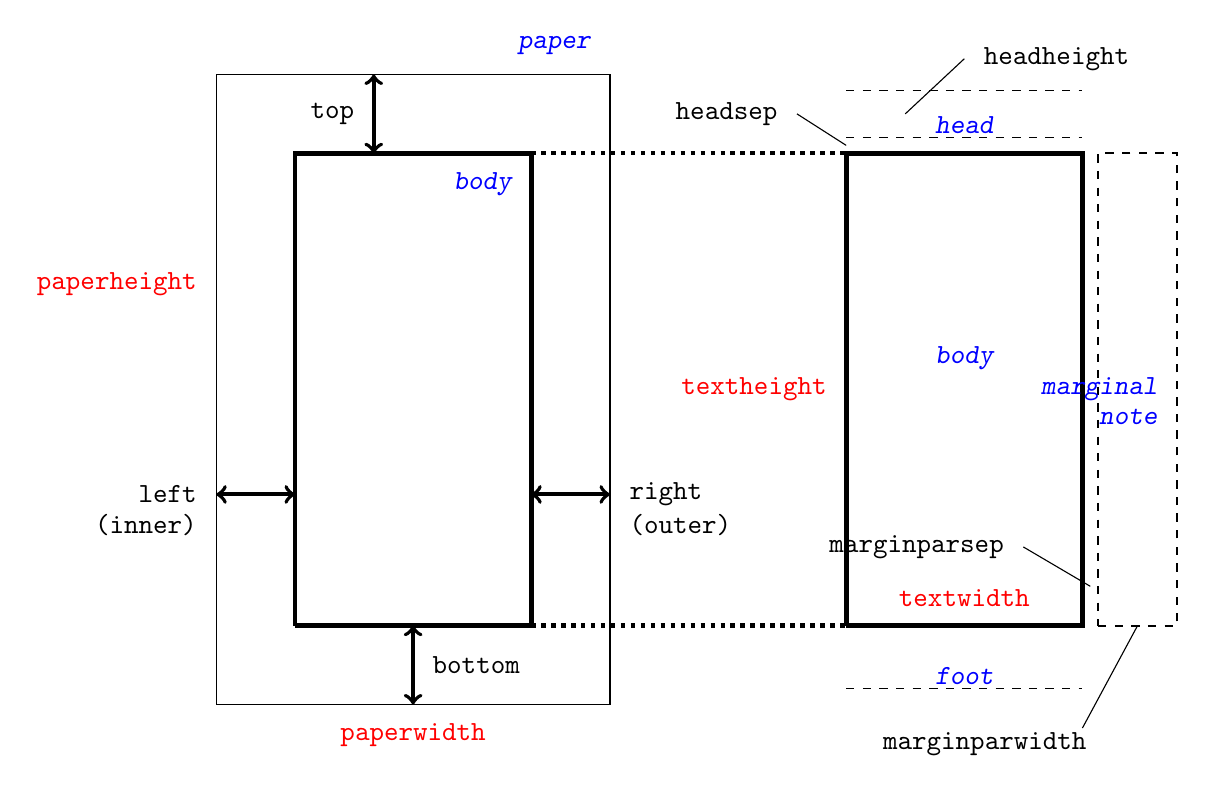
\begin{tikzpicture}{scale=0.9}
% outer-width & outer-height
\newcommand{\owd}{5};
\newcommand{\oht}{8};
% inner-width & inner-height
\newcommand{\iwd}{3};
\newcommand{\iht}{6};
% line length
\newcommand{\len}{5}

% Total Layout
\draw (0,0)--(\owd,0)--(\owd,\oht)--(0,\oht)--(0,0);
\draw[line width=0.06cm] (1,1)--(1+\iwd,1)--(1+\iwd,1+\iht)--(1,1+\iht)--(1,1);
\draw[ultra thick,dotted] (1+\iwd,1+\iht)--(\iwd+\len,1+\iht);
\draw[ultra thick,dotted] (1+\iwd,1)--(\iwd+\len,1);
% Arrow
\draw[<->,line width=0.05cm] (0,1/3*\oht)--(1,1/3*\oht);
\node[label=180:\texttt{left}] at (0,1/3*\oht){};
\node[label=225:\texttt{(inner)}] at (0,1/3*\oht){};
\draw[<->,line width=0.05cm] (1+\iwd,1/3*\oht)--(2+\iwd,1/3*\oht);
\node[label=0:\texttt{right}] at (2+\iwd,1/3*\oht){};
\node[label=315:\texttt{(outer)}] at (2+\iwd,1/3*\oht){};
\draw[<->,line width=0.05cm] (1+\iwd/2,1)--(1+\iwd/2,0);
\node[label=0:\texttt{bottom}] at (1+\iwd/2,0.5){};
\draw[<->,line width=0.05cm] (1+\iwd/3,1+\iht)--(1+\iwd/3,\oht);
\node[label=180:\texttt{top}] at (1+\iwd/3,1/2+\iht/2+\oht/2){};
% Outer Page Label
\node[label=135:\color{blue}{\ttfamily\slshape{paper}}] at (\owd,\oht){};
\node[label=225:\color{blue}{\ttfamily\slshape{body}}] at (1+\iwd,1+\iht){};

% Inner Page
\newcommand{\inn}{\iwd+\len};
\draw[line width=0.06cm] (\inn,1)--(\inn+\iwd,1)--(\inn+\iwd,1+\iht)--(\inn,1+\iht)--(\inn,1);
\node[label=180:\color{red}{\ttfamily{textheight}}] at (\inn,1+\iht/2){};
\node[label=90:\color{red}{\ttfamily{textwidth}}] at (\inn+\iwd/2,1){};
% Margin
\newcommand{\marsep}{0.2}
\newcommand{\marwd}{1}
\newcommand{\mar}{\inn+\iwd+\marsep}
\draw[thick,dashed] (\mar,1)--(\mar+\marwd,1)--(\mar+\marwd,1+\iht)--(\mar,1+\iht)--(\mar,1);
\draw (\mar-\marsep/2,1.5)--(\inn+3/4*\iwd,2);
\node[label=180:\texttt{marginparsep}] at (\inn+3/4*\iwd,2){};
\draw (\mar+\marwd/2,1)--(\inn+\iwd,-0.3);
\node[label=180:\texttt{marginparwidth}] at (\mar+\marsep/2,-0.5){};
% Foot
\draw[dashed] (\inn,0.2)--(\inn+\iwd,0.2);
\node[label=90:\color{blue}{\ttfamily\slshape{foot}}] at (\inn+\iwd/2,0){};
% Head
\draw[dashed] (\inn,1+\iht+0.8)--(\inn+\iwd,1+\iht+0.8);
\draw[dashed] (\inn,1+\iht+0.2)--(\inn+\iwd,1+\iht+0.2);
\node[label=90:\color{blue}{\ttfamily\slshape{head}}] at (\inn+\iwd/2,1+\iht){};
\draw (\inn,1+\iht+0.1)--(\inn-\len/8,1+\iht+0.5);
\node[label=180:\texttt{headsep}] at (\inn-\len/8,1+\iht+0.5){};
\draw (\inn+\iwd/4,1+\iht+0.5)--(\inn+\iwd/2,1+\iht+1.2);
\node[label=0:\texttt{headheight}] at (\inn+\iwd/2,1+\iht+1.2){};

% Total
\node[label=180:\color{red}{\ttfamily{paperheight}}] at (0,2/3*\oht){};
\node[label=270:\color{red}{\ttfamily{paperwidth}}] at (\owd/2,0){};
\node[label=\color{blue}{\ttfamily\slshape{body}}] at (\inn+\iwd/2,1+\iht/2){};
\node[label=180:\color{blue}{\ttfamily\slshape{marginal}}] at (\mar+\marwd,1+\iht/2){};
\node[label=225:\color{blue}{\ttfamily\slshape{note}}] at (\mar+\marwd,1+\iht/2){};
\end{tikzpicture}
\figcaption{页面构成示意图}
\label{fig:geo-paper}
\end{figure}

geometry宏包的具体的选项参数有:
\begin{para}
\item[paper=<papername>]: 其中纸张尺寸有[a0--a6, b0--b6, c0--c6]paper, ansi[a--e]paper, letterpaper, executivepaper, legalpaper.
\item[papersize=\{<width>,<height>\}]: 自定义尺寸。也可以单独对paperwidth或者paperheigth赋值。
\item[landscape]: 切换到横向纸张。默认的是portrait.
\end{para}

body部分分为两个概念:一个是总文本区(total body),另一个是主文本区(body). 总文本区可以由主文本区加上页眉(head)、页脚(foot)、侧页边(marginalpar)组成。默认的选项为includehead,表示总文本区包含页眉。要包括其他内容,可使用:\texttt{includefoot, includeheadfoot, includemp, includeall},以及以上各个参数将include改为ignore后的参数。

总文本区在默认状态下占纸张总尺寸的0.7,由scale=0.7控制,你也可以分别用\texttt{hscale}和\texttt{vscale}指定宽和高的占比。用具体的长度定义也是可以的,使用\texttt{(total)width}和\texttt{(total)height}定义总文本区尺寸,或者用\texttt{textwidth}和\texttt{textheight}定义主文本区的尺寸\footnote{当totalwidth和textwidth都定义时,优先采用后者的值。}。或者直接用\texttt{total=\{width,height\}, body=\{width,height\}}定义。甚至你可以用\texttt{lines=<num>}行数指定textheight。

页边的控制最为常用,分别用\texttt{left/inner, right/outer, top, bottom}来定义四向的页边。其中\texttt{inner, outer}参数只在文档的twoside参数启用时才有意义。你可以用\texttt{hmarginratio}来给定left(inner)与right(outer)页边宽的比例,默认是单页1:1、双页2:3。top和bottom之间的比由\texttt{vmarginratio}给定。你也可以用\texttt{vcentering, hcentering, centering}来指定页边比例为1:1. 在文档的左侧(内侧),可以指定装订线宽度\texttt{bindingoffset},使页边不会被侵入。

页眉和页脚是位于top和bottom页边之内的文档元素。对于页眉和页脚的高度,分别使用\texttt{headheight/head, footskip/foot}参数指定。\texttt{hmargin, vmargin}来指定侧两和顶底的边距。它们到主文本区的参数分别是\texttt{headsep, footnotesep, marginparsep}. 你可以用\texttt{nohead, nofoot, nomarginpar}参数来清除总文本区中的页眉,页脚和侧页边。

对于在文档类documentclass命令中能使用的参数,geometry有不少也能做。比如\texttt{twoside, onecolumn, twocolumn}。甚至还能用文档类中不能用的\texttt{columnsep}(启用多栏分隔线)。

最后,这是几个小例子:
\begin{latex}
% 与Microsoft Word的默认样式相同:
\usepackage[hmargin=1.25in,vmargin=1in]{geometry}
% 书籍中靠书脊一侧的边距较小:
\usepackage[inner=1in,outer=1.25in]{geometry}
\end{latex}

\subsection{页眉和页脚}
页眉和页脚的控制主要借助fancyhdr宏包。\LaTeX\ 中的页眉页脚定义主要借助了两个命令,一个是\latexline{pagestyle},参数有:
\begin{para}
\item[empty] 无页眉页脚。
\item[plain] 无页眉,页脚只包含一个居中的页码。
\item[headings] 无页眉,页脚包含章/节名称与页码。
\item[myheadings] 无页眉,页脚包含页码和用户定义的信息。
\end{para}

另一个命令是\latexline{pagenumbering},与计数器一样,拥有\texttt{arabic, [Rr]oman, [Aa]lph}五种页码形式。

\pkg{fancyhdr}宏包给出了一个叫fancy的\latexline{pagestyle},将页眉和页脚分别分为左中右三个部分,分别叫\latexline{lhead}, \latexline{chead}, \latexline{rhead}, 以及类似的[lcr]foot. 页眉页脚处的横线粗细也可以定义,默认页眉为0.4pt、页脚为0pt. 下面是一个例子:
\begin{latex}
\usepackage{fancyhdr}
\pagestyle{fancy}
    \lhead{}
    \chead{}
    \rhead{\bfseries wklchris}
    \lfoot{Leftfoot}
    \cfoot{\thepage}
    \rfoot{Rightfoot}
\renewcommand{\headrulewidth}{0.4pt}
\renewcommand{\footrulewidth}{0.4pt}
\end{latex}

加载这个宏包,更多地是为了解决双页(twoside)文档的排版问题。对于双页文档,\pkg{fancyhdr}宏包给出了一套新的指令:用E, O表示单数页和双数页,L, C, R表示左中右,H, F表示页眉和页脚。其中H, F需要配合\latexline{fancyhf}命令使用。如果不使用H, F这两个参数,也可以使用\latexline{fancyhead},  \latexline{fancyfoot}两个命令代替。一个新的例子:
\begin{latex}
\fancyhead{} % 清空页眉
    \fancyhead[RO,LE]{\bfseries wklchris}
\fancyfoot{} % 清空页脚
    \fancyfoot[LE,RO]{Leftfoot}
    \fancyfoot[C]{\thepage}
    \fancyfoot[RE,LO]{Rightfoot}
\end{latex}

该宏包在定义双页文档时,采用了如下的默认设置:
\begin{latex}
\fancyhead[LE,RO]{\slshape \rightmark}
\fancyhead[LO,RE]{\slshape \leftmark}
\fancyfoot[C]{\thepage}
\end{latex}

上例中的\latexline{rightmark}表示较低级别的信息,即当前页所在的section,形式如“1.2 sectionname ”,对于article则是subsection;而\latexline{leftmark}表示较高级别的信息,即对应的chapter,对于article则是section. 命令\latexline{leftmark}包含了页面上\latexline{markboth}\footnote{\latexline{markboth}是一个会被\latexline{chapter}等命令调用的命令,默认右参数是空。注意,带星号的大纲不调用这一命令,你需要这样书写:\latexline{chapter*\{This\char`\\markboth\{This\}\{\}\}}。}下的最后一条命令的左参数,比如该页上出现了section 1--2,那么leftmark就是“Section 2”;命令\latexline{rightmark}则包含了页面上的第一个\latexline{markboth}命令的右参数或者第一个\latexline{markright}命令的唯一参数,比如可能是“Subsection 1.2”。

这听起来可能难以理解,但是\latexline{markboth}命令有两个参数,分别对应显示在文档的左页和右页(但是默认右参数留空,用\latexline{markright}去指定右页),故有左右之分;而\latexline{markright}命令只有一个参数。你可以试着再去理解一下双页文档下的宏包的默认设置。利用这一点来重定义chaptermark(book/report), sectionmark, subsectionmark(article)命令,举个例子:
\begin{latex}
% 这里的参数#1是指输入的section/chapter的标题
% 效果:“1.2. The section”
\renewcommand{\sectionmark}[1]{\markright{\thesection.\ #1}}
% 效果:“CHAPTER 2. The chapter”
\renewcommand{\chaptermark}[1]{\markboth{\MakeUppercase{%
    \chaptername}\ \thechapter.\ #1}{}}
\end{latex}

如果你对于默认的\latexline{pagestyle}不满意,可以用\latexline{fancypagestyle}命令进行更改。例如更改plain页面类型:
\begin{latex}
\fancypagestyle{plain}{
    \fancyhf{} % 清空页眉页脚
    \fancyhead[c]{\thesection}
    \fancyfoot{\thepage}}
\end{latex}

\section{抄录与代码环境}
抄录是指将键盘输入的字符(包括保留字符和空格)不经过\TeX\ 解释,直接输出到文档。默认的字体参数是等宽字族(ttfamily)。用法是\latexline{verb(*)}命令或者\envi{verbatim(*)}环境,区别在于带星号的会将空格以“\textvisiblespace”(\latexline{textvisiblespace})的形式标记出来。

注意,\latexline{verb}命令是一个特殊的命令,可以用一组花括号括住抄录内容,也可以任意两个同样的符号(但不能是*)。比如:
\begin{latex}
\verb|fooo{}bar|
\verb+fooo{}bar+
\end{latex}

\latexline{verb(*)}以及\envi{verbatim(*)}环境很脆弱,不能隐式地用于自定义环境,也一般不能用作命令的参数。\pkg{verbatim}宏包提供了更多的抄录支持,\pkg{fancyvrb}宏包提供了\latexline{SaveVerb}, \latexline{UseVerb}命令,以及便于实现居中的\envi{BVerbatim}环境(置于\envi{center}环境内即可),详情读者可自行查阅。

宏包\pkg{shortverb}支持以一对符号代替\latexline{verb}命令,比如竖线号:
\begin{latex}
% \usepackage{shortverb}
\MakeShortVerb|
Verbatim between this pair of verts: |#\?*^|
\end{latex}

代码环境的输出,比如本文中带行号的代码块,参见\hyperref[sec:coding]{这一节}。

\begin{multicols}{2}[\section{分栏}]
这部分内容使用文档类的\texttt{two\-column}可选参数就能实现。在\LaTeX\ 的双栏模式下,\latexline{newpage}命令只能进行换栏操作,而\latexline{clearpage}命令才会换进行换页操作。同时,文中随时可以使用\latexline{twocolumn}或者\latexline{onecolumn}命令执行\RED{换页、清空浮动队列,并切换分栏模式}。在双栏上方的跨栏内容,如摘要,可以写在\latexline{twocolumn[\ldots]}可选参数中。

栏之间的间距由\latexline{columnsep}控制;栏宽为\latexline{columnwidth},但请不要手工修改这个值。它可以被用作参数传递给其他命令。栏之间的分隔线宽由长度\latexline{columnseprule}给出,默认值为0pt,一般需要可以将其设置为0.4pt。 

如果在同一页内需要分栏与单栏并存,或者想要分成多栏,可以尝试使用\pkg{multicol}宏包。它提供一个支持任意多栏、但是边注和浮动体\footnote{带星号的浮动体或许可以使用,如\envi{figure*},但参数\texttt{h}会失效。}无法使用的环境。比如本节:
\begin{latex}
\begin{multicols}{2}
  [\section{分栏}]
  ...
\end{multicols}
\end{latex}

同时,该宏包会对齐每一栏的下边缘;在该环境下,使用\latexline{columnbreak}来强制切换到新的一栏。还需要指出的是,该宏包并不保证各栏之间每行的网格都是对齐的。如果你需要此功能,可以参考\pkg{grid}宏包。
\end{multicols}

\section{文档拆分}
\label{sec:include}
文档拆分只需要在主文件中使用\latexline{input\{filename.tex\}}或\latexline{include\{filename\}}命令,后者不写扩展名默认为.tex。两者区别在于\latexline{include}命令将会插入\latexline{clearpage}再读取文件。

拆分的优势在于可以根据chapter(或其他)分为多个文件,省去了长文档浏览时的一些不便。你也可以把整个导言区做成一个文件,然后在不同的\LaTeX\ 文档中反复使用,即充当模板的功能。你还可以把较长的tikz绘图代码写到一个tex中,在需要时\latexline{input}即可。

在导言区定义\latexline{includeonly}加上filename,可以确保只引入列表中的文件。在被引入文件的最后加入\latexline{endinput}命令,其后的内容会被忽略。

一种较规范的拆分文件的文件头,以本文的章节放在次级目录中为例:
\begin{latex}
%!TEX root = ../LaTeX-cn.tex
\end{latex}

\section{西文排版及其他}
\subsection{连写}
\LaTeX\ 排版以及正规排版中,如果你输入ff, fl, fi, ffi等内容,它们默认会连写。在字母中间插入空白的箱子以强制不连写:f~\latexline{mbox\{\}}~l。

\subsection{断词}
行末的英文单词太长,\LaTeX\ 就会以其音节断词。如果你想指定某些单词的断词位置,使用如下命令断词。例子:
\begin{latex}
\hyphenation{Hy-phen-a-tion FORTRAN}
\end{latex}

这个例子允许Hyphenation, hyphenation在短横处断词,同时\textbf{禁止}FORTRAN, Fortran, fortran断词。如果你在行文中加入\verb|\-|命令,则可以实现允许在对应位置断词的效果。比如:

\begin{codeshow}
I will show you this:
su\-per\-cal\-i\-frag\-i\-lis\-%
tic\-ex\-pi\-al\-i\-do\-cious
\end{codeshow}

如果你不想断词,比如电话号码,巧妙利用\latexline{mbox}命令吧:
\begin{latex}
My telephone number is: \mbox{012 3456 7890}
\end{latex}

\subsection{硬空格与句末标点}
如果你想在某个不带参数的命令后输入空格,请接上一个空的花括号确保空格能够正常输出。例如:\latexline{这是\char`\\TeX\{\} Live. }

在\LaTeX\ 中还有一个命令“\texttt{\char92\textvisiblespace}”,用于产生一个硬空格(区别于软空格\texttt{\char92space}),所以你也可以用\latexline{TeX\char`\\ \textvisiblespace Live}。

西文排版下,\LaTeX\ 会判断一种\co{句末标点},即小写字母后的“.”,“?”或者“!”三个英文标点。句末标点后如果键入空格,\LaTeX\ 会自动增加空格的距离。如果句子以大写字母结尾,\LaTeX\ 会认为这是人名而不增加空格,这时候需要手动添加命令\latexline{@}:

\begin{codeshow}
OK. That's fine.\\
OK\@. That's fine.
\end{codeshow}

相反,有些并非句末标点的情况会被识别为句末标点,这时候需要在标点后插入一个\latexline{\textvisiblespace}或者\verb|~|来缩小间距;区别在于前者允许断行,后者不允许。

\begin{codeshow}
Prof. Smith is a nice man.\\
Prof.~Smith is a nice man.
\end{codeshow}

在标点后使用\latexline{frenchspacing}命令,可以调整为极小的空距。这个命令在排版参考文献列表时可能被使用。

在\xelatex 编译模式下的中文字符,与西文或者符号之间会产生默认的空距\footnote{这个问题在ctex文档类下似乎被已解决。}。如果你不想要这个空距,把中文放在\latexline{mbox}内即可,比如:

\begin{codeshow}
\mbox{例子}-1
\end{codeshow}

\subsection{特殊符号}
符号的总表可以参照symbols-a4文档,运行texdoc symbols-a4即可调出。包括希腊字母在内的一些数学符号将会在下一章介绍。这里给出基于\pkg{wasysym}宏包的一些常用符号:
\begin{center}
  \centering
  \tabcaption{wasysym宏包符号}
  \begin{tabular}{*{3}{c >{\ttfamily\char92}p{5.5em}}}
     \permil     & permil   & \male     & male  & \female       & female \\
     \checked    & checked  & \XBox     & XBox  & \CheckedBox   & CheckedBox \\
     \hexstar    & hexstar  & \phone    & phone & \twonotes     & twonotes
  \end{tabular}
\end{center}

%!TEX root = ../LaTeX-cn.tex
\chapter{数学排版}
\section{行间与行内公式}
\co{行内公式}指将公式嵌入到文段的排版方式,主要要求公式垂直距离不能过高,否则影响排版效果。行内公式的书写方式:
\begin{latex}
$...$ 或者 \(...\) 或者 \begin{math}...\end{math}
\end{latex}

一般推荐第一或第二种方式。例:\verb|$\sum_{i=1}^{n}a_i$|,即:$\sum_{i=1}^{n}a_i$.

另外一种公式排版方式是\co{行间公式},也称行外公式,使用:
\begin{latex}
\[...\] 或者 \begin{displaymath}...\end{displaymath}
或者 amsmath 提供的 \begin{equation*}...\end{equation*}
\end{latex}

一般也推荐第一种命令\footnote{还有一种\texttt{\$\$...\$\$}的写法,源自底层\TeX,不建议使用。},例如:\verb|\[\sum_{i=1}^n{a_i}\]|,得到:
\[\sum_{i=1}^{n}a_i\]

从上面的两个例子可以看出,即使输出相同的内容,行内和行间的排版也是有区别的,比如累加符号上标是写在正上方还是写在右上角。

如果行间公式需要编号,使用\envi{equation}环境\footnote{需要注意有一个\RED{已被放弃}的多行公式编号环境叫\texttt{eqnarray},请不要再使用。},还可以插入标签:

\begin{codeshow}
\begin{equation}
\label{eq:NoExample}
  |\epsilon|>M
\end{equation}
\end{codeshow}

\section{数学字体、字号与空格}
\label{sec:mathfont}
\subsection{空格}
在数学环境中,行文空格是被忽略的。比如\verb|$x,y$|和\verb|$x, y$|并没有区别。数学环境有独有的空格命令,最后一个是$-3/18$的空格:

\begin{codeshow}
  $没有空格,3/18空\,格$ \\
  $4/18空\:格,5/18空\;格$ \\
  $9/18空\ 格,一个空\quad 格$ \\
  $两个空\qquad 格,负3/18空\!格$
\end{codeshow}

事实上,以上命令也可以在数学模式外使用,其中使用最广泛的是\latexline{,},比如上文提到过的千位分隔符。在数学环境中它也应用广泛(含有隐式的\latexline{,}):

\begin{codeshow}
\[ \int_0^1 x \ud{}x
= \frac{1}{2} \]
\end{codeshow}

其中\verb|\ud|命令是自定义的,这也是微分算子的正常定义\label{cmd:ud}:
\begin{latex}
\newcommand{\ud}{\mathop{}\negthinspace\mathrm{d}}
\end{latex}

\subsection{间距}
命令\latexline{abovedisplayskip}和\latexline{belowdisplayskip}控制了行间公式与上下文之间的间距,并且该值不会随字号调整而调整。有时你需要自行指定。默认值\texttt{12pt plus 3pt minus 9pt}。多行公式之间的间距用\latexline{jot}来控制,默认\texttt{3pt}。命令\latexline{mathsurround}给出了行内公式与文字间,除了预留空格之外的间距,默认值为\texttt{0pt}。另外一个有趣的命令\latexline{smash},可以忽略参数的全高:
\begin{codeshow}
\[\underline{\smash{\int f(x)\ud x}}=1\]
\end{codeshow}

也能够通过参数,选择只忽略高度(t)或只忽略深度(b):
\begin{codeshow}
$\sqrt{A_{n_k}} \qquad
\sqrt{\smash[b]{A_{n_k}}}$
\end{codeshow}

\subsection{字号}
\LaTeX\ 提供四种字号尺寸命令:
\begin{para}
\item[\latexline{displaystyle}] 行间公式尺寸。如$\displaystyle \sum_{i=1}^n a$
\item[\latexline{textstyle}] 行内公式尺寸。如$\textstyle \sum_{i=1}^n a$
\item[\latexline{scriptstyle}] 上下标尺寸。如$\scriptstyle \sum_{i=1}^n a$
\item[\latexline{scriptscriptstyle}] 次上下标尺寸。如$\scriptscriptstyle \sum_{i=1}^n a$
\end{para}

\subsection{数学字体}
将字体转为正体使用\latexline{mathrm}命令。如需保留空格,使用\latexline{textrm}命令——这与正文一致。但是,\latexline{textrm}命令内的字号可能不会自适应,\latexline{mathrm}则表现起来稳定得多。

例如自然对数的底数$\ue$,在本文中就是这样定义的:
\begin{latex}
\newcommand{\ue}{\mathrm{e}}
\end{latex}

以下简单介绍几种数学字体。数学字体的总表参见\tref{tab:mathfont}。

\subsubsection{数学粗体}
数学粗体使用\pkg{amsmath}宏包支持的\latexline{boldsymbol}命令。命令\latexline{boldmath}的问题在于它只能加粗一个数学环境,其中很可能包括了标点符号,而这是不严谨的。命令\latexline{mathbf}就差的更远,它只能把字体转为\textbf{正}粗体,而数学字体都是斜体的。

\begin{codeshow}
$\mu,M$\\ $\boldsymbol{\mu},
\boldsymbol{M}$
\end{codeshow}

\subsubsection{空心粗体}
空心粗体使用\pkg{amsfonts}或\pkg{amssymb}宏包的\latexline{mathbb}命令。这里用\latexline{textrm}而不是\latexline{mathrm},是为了保留空格。

\begin{codeshow}
$x^2 \geq 0 \qquad
\textrm{for all }x\in\mathbb{R}$
\end{codeshow}

\section{基本命令}
基本函数默认用正体书写,包括:
\begin{verbatim}
\sin \cos \tan \cot \arcsin \arccos \arctan \cot \sec \csc
\sinh \cosh \tanh \coth \log \lg \ln \ker \exp \dim \arg \deg 
\lim \limsup \liminf \sup \inf \min \max \det \Pr \gcd
\end{verbatim}

以上函数,最后一行的10个是可以带上下限参数的,即在行间公式模式下,上标和下标将在函数正上方和正下方书写内容。

\pkg{amsmath}宏包允许\latexline{DeclareMathOperator}命令自定义基本函数,用法类似于\latexline{newcommand}命令。如果命令带星号\latexline{DeclareMathOperator*},则可以带上下限参数。

此外有一个叫\latexline{mathop}的命令,可以把参数转换为数学对象,使其能够堆叠上下标;\latexline{mathbin}与\latexline{mathrel}则分别能把参数转换为二元运算符、二元关系符,并正确设置两侧的空距。

\subsection{上下标与虚位}
用低划线和尖角符表示上标和下标,请仔细体会下述例子:

\begin{codeshow}
$a^3_{ij}$ \\
${a_{ij}}^3\text{或}a_{ij}{}^3$\\
$\mathrm{e}^{x^2}\geq 1$
\end{codeshow}

上面的指数3的位置读者可以多多体会一下。此外,\latexline{phantom}被称为虚位命令,从下例你也能够体会到他的作用:

\begin{codeshow}
${}^{12}_{6}\mathrm{C}$ \\
${}^{12}_{\phantom{1}6}
\mathrm{C}$ \\
$a^3_{ij}$ \\
$a^{\phantom{ij}3}_{ij}$
\end{codeshow}

宏包\pkg{mathtools}提供了\latexline{prescript}来避免手工调整:
\begin{codeshow}
$\prescript{12}{6}{\mathrm{C}}$
\end{codeshow}

\subsection{微分与积分}
导数直接使用单引号\verb|'|,积分使用\latexline{int}符号:

\begin{codeshow}
$y'=x \qquad \dot{y}(t)=t$ \\
$\ddot{y}(t)=t+1$
$\dddot{y}+\ddddot{y}=0$ \\
$\iint_{D}f(x)=0$
$\int_{0}^{1}f(x)=1$
\end{codeshow}

有时候需要更高级的微分或积分号,其中\latexline{ud}命令在\hyperref[cmd:ud]{上文这里}定义过:
\begin{codeshow}
\[\left.\frac{\ud y}{\ud x}\right|_{x=0}\quad
\frac{\partial f}{\partial x}
\quad\oint\;\varoiint_S \]
\end{codeshow}

其中的\latexline{dot}系的导数形式\LaTeX\ 只原生支持到二阶导数。后面的三阶、四阶需要\pkg{amsmath}宏包。\latexline{int}系的积分命令类似。而环形双重积分命令\latexline{varoiint}需要\pkg{esint}宏包\footnote{该宏包可能与\pkg{amsmath}冲突,即便使用也请其放在\pkg{amsmath}之后加载。}。

\latexline{left.}或\latexline{right.}命令\footnote{参考\hyperref[subsec:delimiter]{定界符}部分的内容。}只用于匹配,本身不输出任何内容。

\subsection{分式、根式与堆叠}
分式使用\latexline{frac}命令。或者\pkg{amsmath}宏包支持的\latexline{dfrac}、\latexline{tfrac}命令来强制获得行间公式、行内公式大小的分数。如果想自定义分式样式,参考\secref{subsec:binom}一节的\latexline{genfrac}命令。
\begin{codeshow}
\[\frac{x}{y}+\dfrac{x}{y}
+\tfrac{a}{b}\]
\end{codeshow}

该宏包还支持另一个命令\latexline{cfrac},用于输入连分式。
\begin{codeshow}
\[\cfrac{1}{1+\cfrac{2}{1+x}}\]
\end{codeshow}

空根式用\latexline{surd}输出,更常用的是\latexline{sqrt}:
\begin{codeshow}
$\sqrt{2} \qquad \surd$\\
$\sqrt[\beta]{k}$
\end{codeshow}

开方次数的位置可以用这两个命令微调,参数是整数:
\begin{codeshow}
$\sqrt[\leftroot{-2}\uproot{2} \beta]{k}$
\end{codeshow}

划线命令使用\latexline{underline}和\latexline{overline},水平括号使用brace或者bracket代替line,例如\latexline{underbrace}:

\begin{codeshow}
$\overline{m+n}$ \\
$\underbrace{a_1+\cdots+a_n}_{n}$
$\overbrace{a_1+\cdots+a_n}^{n}$
% 可选参数:线宽;竖直空距
$\underbracket[0.4pt][1ex]
  {a_1+\cdots+a_n}_n$
\end{codeshow}

两个互有重叠的括号需要一个箱子命令\latexline{rlap},会在后面提到。不过在$j$之前的空距有些异常,可能需要\latexline{,}进行修正。
\begin{codeshow}
\[b+\rlap{$\overbrace{\phantom{
  c+d+e+f+g}}^x$}c+d+\underbrace{
  e+f+g+h+i}_y+\,j \]
\end{codeshow}

事实上\latexline{overline}命令也存在问题,请比较:

\begin{codeshow}
$\overline{A}\overline{B}$ \\
$\closure{A}\closure{B}$
$\closure{AB}$
\end{codeshow}

其中\latexline{closure}是在导言区定义的:
\begin{latex}
\newcommand{\closure}[2][3]{{}\mkern#1mu
    \overline{\mkern-#1mu#2}}
\end{latex}

还可以输出能堆叠到其他对象上的箭头符,比如向量符号:

\begin{codeshow}
  $\vec a\quad \overrightarrow{PQ}$
  $\overleftarrow{EF}$
\end{codeshow}

你也许还需要能够添加上下堆叠的箭头符:

\begin{codeshow}
\[ a\xleftarrow{x+y+z} b \]
\[ c\xrightarrow[x<y]{a*b*c}d \]
\end{codeshow}

尖帽符号、波浪符号,还有\pkg{yhmath}宏包支持的圆弧符号:

\begin{codeshow}
$\hat{A}\quad\widehat{AB}$\\
$\tilde{C}\quad\widetilde{CD}
\qquad\wideparen{APB}$
\end{codeshow}

强制堆叠命\latexline{stackrel},位于上方的符号与上标同等大小。如果有\pkg{amsmath}宏包,可以使用\latexline{overset}或者\latexline{underset} 命令,前者与\latexline{stackrel}命令完全等同:

\begin{codeshow}
$\int f(x) \stackrel{?}{=} 1$\\
$A\overset{abc}{=}B$ \quad $C\underset{def}{=}D$
\end{codeshow}

一个很强大的堆叠放置命令\latexline{sideset},只用于巨算符:

\begin{codeshow}
\[\sideset{_a^b}{_c^d}\sum\]
\[\sideset{}{'}\sum_{n=1}\text{或}
\,{\sum\limits_{n=1}}'\]
\end{codeshow}

去心邻域\latexline{mathring}大概也属于堆叠符的一种?这样输出:

\begin{codeshow}
$\mathring{U}$
\end{codeshow}

在下一次节:累加与累积中,还介绍了更多的堆叠命令。

\subsection{累加与累积}
使用\latexline{sum}和\latexline{prod}命令,效果如下:

\begin{codeshow}
\[\sum_{i=1}^{n}a_i=1 \qquad
\prod_{j=1}^{n}b_j=1\]
\end{codeshow}

有时需要复杂的堆叠方式,效果如下:

\begin{codeshow}
\[\sum_{\substack{0<i<n \\
  0<j<m}} p_{ij}=
  \prod_{\begin{subarray}{l}
  i\in I \\  1<j<m
  \end{subarray}}q_{ij}\]
\end{codeshow}

有时候需要强制实现堆叠的效果,可以使用\latexline{limits}命令。如果堆积目标不是数学对象,还需要使用\latexline{mathop}命令:

\begin{codeshow}
\[\max\limits_{i>1}^{x}\quad
\mathop{xyz}\limits_{x>0}\quad
\lim\nolimits_{x\to \infty}\]
\end{codeshow}

\subsection{矩阵与省略号}
最朴素的矩阵排版可以通过\envi{array}环境和自适应定界符完成:

\begin{codeshow}
\[\mathbf{A}=
\left(\begin{array}{ccc}
x_{11} & x_{12} & \ldots \\
x_{21} & x_{22} & \ldots \\
\vdots & \vdots & \ddots
\end{array}\right)\]
\end{codeshow}

还有就是\latexline{cdots}命令。\pkg{mathdots}宏包支持省略号缩放,并提供了\latexline{iddots}:$\iddots$. 或许什么时候需要使用呢?

矩阵排版更多地使用\envi{matrix}环境,以圆括号矩阵\envi{pmatrix}最为常见:
\begin{codeshow}
\centering $\begin{matrix}
0 & 1 \\ 1 & 0 \end{matrix}\qquad
\begin{pmatrix} 0 & 2 \\
2 & 0 \end{pmatrix}$
\end{codeshow}

方括号和花括号使用\envi{[Bb]matrix}环境:
\begin{codeshow}
\centering $\begin{bmatrix}
0 & 3 \\ 3 & 0 \end{bmatrix}\qquad
\begin{Bmatrix} 0 & 4 \\
4 & 0 \end{Bmatrix}$
\end{codeshow}

行列式使用\envi{[Vv]matrix}环境:
\begin{codeshow}
\centering $\begin{vmatrix}
0 & 5 \\ 5 & 0 \end{vmatrix}\qquad
\begin{Vmatrix} 0 & 6 \\
6 & 0 \end{Vmatrix}$
\end{codeshow}

宏包\pkg{mathtools}的带星\texttt{matrix}命令,可更改列对齐:
\begin{codeshow}
$\begin{pmatrix*}[r]
100 & -200 \\ 20 & 10
\end{pmatrix*}$
\end{codeshow}

在矩阵中排版\latexline{dfrac}分式时,处理行距如下例的 \texttt{\char92\char92 [8pt]}:
\begin{codeshow}
\[\mathbf{H}=\begin{bmatrix}
\dfrac{\partial^2 f}{\partial x^2} &
\dfrac{\partial^2 f}
{\partial x \partial y} \\[8pt]
\dfrac{\partial^2 f}
{\partial x \partial y} &
\dfrac{\partial^2 f}{\partial y^2}
\end{bmatrix}\]
\end{codeshow}

宏包\pkg{amsmath}还支持行内小矩阵\latexline{smallmatrix},需手动加括号。
\begin{codeshow}
矩阵 $\left(\begin{smallmatrix}
x & -y\\ y & x\end{smallmatrix}
\right)$ 可以显示在行内。
\end{codeshow}

一种带边注的矩阵\latexline{bordermatrix},用法有些奇怪:
\begin{codeshow}
\[\bordermatrix{& 1 & 2\cr
1 & A & B \cr
2 & C & D \cr} \]
\end{codeshow}

最后,如果想排出更好看优雅的矩阵,可以参考宏包\pkg{nicematrix}。或者想用简单的方法输入一些特殊矩阵, 可以参考宏包\pkg{physics},这里不过多介绍。

\subsection{分段函数与联立方程}
用\envi{cases}环境书写分段函数,它自动生成一个比\latexline{left\{}更紧凑的花括号:

\begin{codeshow}
\[y=\begin{cases}
\int x, & x>0 \\
0,   & x=0 \\
x-1, & x<0
\end{cases},\,x\in\mathbb{R}\]
\end{codeshow}

如果想要生成display样式的内容(比如上面的积分号只是text样式的),使用\pkg{mathtools}宏包的\envi{dcases}环境代替\envi{cases}环境。如果\envi{cases}环境的第二列条件不是数学语言而是一般文字,可以考虑使用\envi{dcases*}环境,列中用\&{}隔开。

\begin{codeshow}
\[y=\begin{dcases}
  \int x, & x>0 \\
  x^2, & x\leqslant 0
  \end{dcases}\]
\[z=\begin{dcases*}
  y, & when $y$ is prime\\
  y^2, & otherwise
  \end{dcases*}\]
\end{codeshow}

\subsection{多行公式及其编号}
\label{subsec:multieqnum}
多行公式可以使用\pkg{amsmath}下的\envi{align}环境——因为原生的\envi{eqnarray}环境真的很差!而且\envi{align}环境不需要像\envi{array}环境那样给出列的数目和参数,能够根据
\texttt{\&}符号的数量来自调整。\qd{这个环境会自动对齐等号或者不等号,所以必要时请用\&指定对齐位置}。下面是一个例子:

\begin{codeshow}
\begin{align}
  a^2  &= a\cdot a \\
       &= a*a      \\
       &= a^2
\end{align}
\end{codeshow}

但是在\envi{align}及其衍生环境中,要将\&放在二元关系符的前面,如果放在后面会导致关系符与后面字母的间距出现问题:

\begin{codeshow}
\begin{align*}
  a^2   &= a\cdot a \\
        &= a*a      
\end{align*}
\begin{align*}
  a^2   =& a\cdot a \\
        =& a*a      
\end{align*}
\end{codeshow}

\LaTeX\ 中长公式不能自动换行\footnote{不过\pkg{breqn}宏包的\envi{dmath}环境可以实现自动换行,读者可以自行尝试效果。},请如上自行指定断行位置和缩进距离。

至于多行公式换页,可以在导言区加上\latexline{allowdisplaybreaks}实现(可选参数:1为尽量避免换页,2至4为倾向于换页),或在特定位置加上\latexline{displaybreak}(可选参数:0为允许在下个换行符后换页,但不倾向换页;2-3介中;4为强制换页)。两种的默认可选参数都是4。

上例给出三个编号,如果你只需要一个,可以:

\begin{codeshow}
\begin{align}
  a^2&= a\cdot a& b&=c\nonumber\\
  g  &= a*a & d&>e>f  \nonumber\\
  step&= a^2 & &Z^3
\end{align}
\end{codeshow}

如果你想让编号显示在这三行的中间而不是最下面一行,可以尝试把公式写在\envi{aligned}或者\envi{gathered}环境中,然后再嵌套到\envi{equation}环境内:

\begin{codeshow}
\begin{equation}
  \begin{aligned}
    a^2  &= a\cdot a \\
         &= a*a      \\
         &= a^2
  \end{aligned}
\end{equation}
\end{codeshow}

如果你根本不想给多行公式编号,尝试\envi{align*}环境。

另外,\pkg{amsmath}宏包的\envi{multline}环境将自动把编号放在末行。首行左对齐,末行右对齐,中间的行居中。
\begin{codeshow}
\begin{multline}
a>b \\
b>c \\
\therefore a>c
\end{multline}
\end{codeshow}

如果想在环境中插入小段行间文字,使用\latexline{intertext}命令,或者\pkg{mathtools}宏包的\latexline{shortintertext}命令。区别是后者的垂直间距更小一些。

\begin{codeshow}
\begin{align*}
\shortintertext{If}
 y &= 0 \\
 x &< 0\\
\shortintertext{then}
 z &= x+y
\end{align*}
\end{codeshow}

当然,\envi{align}环境用于分列对齐的。如果仅想所有行居中,使用\pkg{amsmath}宏包的\envi{gather}环境即可。这是一个非常实用的环境,你也可以用\envi{gather*}环境排版居中的、非编号的多行公式。

\begin{codeshow}
\begin{gather}
  X=1+2+\cdots+n \\
  Y=1
\end{gather}
\end{codeshow}

\subsection{二项式}
\label{subsec:binom}
二项式可能需要借助\pkg{amsmath}宏包的\latexline{binom}命令。它也有像分式一样的行间和行内两个命令\latexline{tbinom}与\latexline{dbinom}:

\begin{codeshow}
$\mathrm{C}_n^k=\binom{n}{k}
\qquad a_n=\dbinom{n}{k}$
\end{codeshow}

你也可以通过该宏包支持的\latexline{genfrac}自定义类似二项式命令:
\begin{latex}
\genfrac{left-delim}{right-delim}{thickness}{mathstyle}
{numerator}{denominator}
% thickness为分式线线宽,留空空表示默认
% mathstyle从0-3由\displaystyle减至\scriptscriptstyle
\newcommand{\Bfrac}[2]{\genfrac{[}{]}{0pt}{}{#1}{#2}}
\end{latex}

你可以借此得到新的命令\latexline{Bfrac}:
\begin{codeshow}
\[\text{We define } \Bfrac{n}{k} = \binom{k}{n}\]
\end{codeshow}

\subsection{定理}
在使用下述定理内容时,请加载\pkg{amsthm}宏包。

首先是定理环境格式的自定义。如同定义命令一样,在导言区加上:
\begin{latex}
\newtheorem{envname}[counter]{text}[section]
\end{latex}

其中\textit{name}表示定理的引用名称,即下文将其作为一个环境名来识别;\textit{text}表示定理的显示名称,即下文中定理将以其作为打印内容。而\textit{counter}参数表示你是否与先前声明的某定理共同编号。\textit{section}参数表示定理的计数层级,如果是section,表示每节分别计数;chapter表示每章分别计数。

来看一个例子。首先在导言区定义如下三个样式:
\begin{latex}
\theoremstyle{definition}\newtheorem{laws}{Law}[section]
\theoremstyle{plain}\newtheorem{ju}[laws]{Jury}
\theoremstyle{remark}\newtheorem*{marg}{Margaret}
\end{latex}

以上三个\latexline{theoremstyle}即是它预定义的所有样式类型。definition标题粗体,内容罗马体;plain标题粗体,内容斜体;remark标题斜体,内容罗马体。带星号表示不进行计数。在环境的使用中可以添加可选参数,用于以括号的形式注释定理。然后这是示例:

\begin{codeshow}
\begin{laws}
Never believe easily.
\end{laws}
\begin{ju}[The 2nd]
Never suspect too much.
\end{ju}
\begin{marg}
Nothing else.
\end{marg}
\end{codeshow}

\pkg{amsthm}宏包还提供了\envi{proof}环境,并且用\latexline{qedhere}来指定证毕符号的位置。如果不加指定,将会自动另起一行。

\begin{codeshow}
\begin{proof}
For an right triangle, we have:
  \[a^2+b^2=c^2 \qedhere\]
\end{proof}
\end{codeshow}

\section{数学符号与字体}
\subsection{数学字体}
原生的数学字体命令:
\begin{center}
\begin{minipage}{\linewidth}
\centering
\tabcaption{原生数学字体表}
\label{tab:mathfont}
\begin{tabular}{>{\ttfamily\char92}l>{$}l<{$}}
\hline
mathrm\{ABCDabcde 1234\} & \mathrm{ABCDabcde 1234} \\
\hline
mathit\{ABCDabcde 1234\} & \mathit{ABCDabcde 123} \\
\hline
mathnormal\{ABCDabcde 1234\} & \mathnormal{ABCDabcde 1234} \\
\hline
mathcal\{ABCDabcde 1234\} & \mathcal{ABCDabcde 1234} \\
\hline
\end{tabular}
\end{minipage}
\end{center}

需要其他宏包支持的数学字体:
\begin{center}
\begin{minipage}{\linewidth}
\centering
\tabcaption{宏包数学字体表}
\label{tab:mathfont-pk}
\begin{tabular}{>{\ttfamily}ll}
\hline
\char92mathscr\{ABCDabcde 1234\} & mathrsfs\\
$\mathscr{ABCDabcde 1234}$ & \\
\hline
\char92mathfrak\{ABCDabcde 1234\} & amsfonts或者amssymb\\
$\mathfrak{ABCDabcde 1234}$ & \\
\hline
\char92mathbb\{ABCDabcde 1234\} & amsfonts或者amssymb\\
$\mathbb{ABCDabcde 1234}$ & \\
\hline
\end{tabular}
\end{minipage}
\end{center}

\subsection{定界符}
\label{subsec:delimiter}
\tref{tab:delimiter}给出了一些数学环境中使用的定界符。

\begin{table}[!htb]
\centering
\caption{定界符}
\label{tab:delimiter}
\begin{tabular}{@{}*{3}{>{$}p{2em}<{$} @{} >{\ttfamily}p{7em}}}
( & ( & [ & [ or \char92 lbrack & \uparrow & \char92 uparrow \\
) & ) & ] & ] or \char92 rbrack & \downarrow & \char92 downarrow \\
\{ & \{ or \char92 lbrace & \} & \} or \char92 rbrace & \updownarrow & \char92 updownarrow \\
\langle & \char92 langle & \rangle & \char92 rangle & \backslash & \char92 backslash \\
\lfloor & \char92 lfloor & \rfloor & \char92 rfloor & \Updownarrow & \char92 Updownarrow \\
\lceil & \char92 lceil & \rceil & \char92 rceil & \Uparrow & \char92 Uparrow \\
\Vert & \char92 | or \char92 Vert & | & | or \char92 vert & \Downarrow & \char92 Downarrow \\
\hline
\multicolumn{6}{c}{-- 以下需要amssymb宏包 --} \\
\multicolumn{3}{c}{$\ulcorner$ \quad \texttt{\char92 ulcorner}} & \multicolumn{3}{c}{$\urcorner$ \quad \texttt{\char92 urcorner}} \\
\multicolumn{3}{c}{$\llcorner$ \quad \texttt{\char92 llcorner}} & \multicolumn{3}{c}{$\lrcorner$ \quad \texttt{\char92 lrcorner}}
\end{tabular}
\end{table}

使用\latexline{left}, \latexline{right}还有\latexline{middle}能够使定界符自适应式子的高度:
\begin{codeshow}
\[P\left(X \middle\vert Y=0\right)
=\left.\int_0^1 p(t)\ud t\middle/ N\right.\]
\end{codeshow}

如果希望手动指定定界符的尺寸,这时使用后:
\begin{codeshow}
% 加l, r, m对应上述三种自适应命令
$(\big(\Big(\bigg(\Bigg<\qquad
\bigl[\frac{x+y}{x^2}\bigr]$
\end{codeshow}

有时\latexline{left.}和\latexline{right.}能灵活地用于跨行控制,因为它们并非实际配对:
\begin{codeshow}
\begin{align*}
  x &=\left(\frac{1}{2}x\right.\\
  &\left.\vphantom{\frac{1}{2}}
  +y^2+z_1\right)
\end{align*}
\end{codeshow}

其中\latexline{vphantom}命令用于输出一个高度虚位,使得第二行的自适应定界符与第一行同等大小。特别地,命令\latexline{mathstrut}表示一个有圆括号总高的虚位:
\begin{codeshow}
$\sqrt{b}\sqrt{y}\qquad
\sqrt{\mathstrut b}\sqrt{\mathstrut y}$
\end{codeshow}

\subsection{希腊字母}
希腊字母表如\tref{tab:greekletter}所示。表中包含了小写希腊字母、大写希腊字母,其中部分希腊字母的输入方式与英文字母一致。
\begin{table}[!htb]
\centering
\caption{希腊字母表}
\label{tab:greekletter}
\renewcommand\arraystretch{1}
\begin{tabular}{*{4}{>{$}c<{$}!{}>{\ttfamily\char`\\}p{6em} @{}}}
\alpha & alpha & \theta & theta & o & \multicolumn{1}{p{6em}}{o} & \upsilon & upsilon \\
\beta & beta & \vartheta & vartheta & \pi & pi & \phi & phi \\
\gamma & gamma & \iota & iota & \varpi & varpi & \varphi & varphi \\
\delta & delta & \kappa & kappa & \rho & rho & \chi & chi \\
\epsilon & epsilon & \lambda & lambda & \varrho & varrho & \psi & psi \\
\varepsilon & varepsilon & \mu & mu & \sigma & sigma & \omega & omega \\
\zeta & zeta & \nu & nu & \varsigma & varsigma & \eta & eta \\
\xi & xi & \tau & tau & \multicolumn{4}{c}{} \\
A & \multicolumn{1}{p{6em}}{A} & B & \multicolumn{1}{p{6em}}{B} & \Gamma & Gamma & \varGamma & varGamma \\
\Delta & Delta & \varDelta & varDelta & E & \multicolumn{1}{p{6em}}{E} & Z & \multicolumn{1}{p{6em}}{Z} \\
H & \multicolumn{1}{p{6em}}{H} & \Theta & Theta & \varTheta & varTheta & I & \multicolumn{1}{p{6em}}{I} \\
\Lambda & Lambda & \varLambda & varLambda & M & \multicolumn{1}{p{6em}}{M} & N & \multicolumn{1}{p{6em}}{N} \\
\Xi & Xi & \varXi & varXi & O & \multicolumn{1}{p{6em}}{O} & \Pi & Pi \\
\varPi & varPi & P & \multicolumn{1}{p{6em}}{P} & \Sigma & Sigma & \varSigma & varSigma \\
T & \multicolumn{1}{p{6em}}{T} & \Upsilon & Upsilon & \varUpsilon & varUpsilon & \Phi & Phi \\
\varPhi & varPhi & X & \multicolumn{1}{p{6em}}{X} & \Psi & Psi & \varPsi & varPsi \\
\Omega & Omega & \varOmega & varOmega & \multicolumn{4}{c}{}
\end{tabular}
\end{table}

\subsection{二元运算符}
二元运算符包括常见的加减乘除,还有集合的交、并、补等运算。\tref{tab:operator}只列出常用的二元运算符,更多的请参考symbols-a4文档。
\begin{table}[!htb]
\centering
\caption{二元运算符:\latexline{mathbin}}
\label{tab:operator}
\renewcommand\arraystretch{1}
\begin{tabular}{@{}*{2}{>{$}c<{$}!{} >{\ttfamily\char92}p{5em} @{}}*{2}{>{$}p{2em}<{$} @{} >{\ttfamily\char92}p{6em} @{}}}
+ & \multicolumn{1}{p{6em}}{+} & - & \multicolumn{1}{p{6em}}{-} & \times & times & \div & div \\
\pm & pm & \mp & mp & \circ & circ & \triangleright & triangleright \\
\cdot & cdot & \star & star & \ast & ast & \triangleleft & triangleleft \\
\cup & cup & \cap & cap & \setminus & setminus & \bullet & bullet \\
\oplus & oplus &\ominus & ominus & \otimes & otimes & \oslash & oslash \\
\odot & odot & \bigcirc & bigcirc & \vee & vee,lor & \wedge & wedge,land \\
\bigcup & bigcup & \bigcap & bigcap & \bigvee & bigvee & \bigwedge & bigwedge
\end{tabular}
\end{table}

\subsection{二元关系符}
二元关系符常常被用于判断两个数的大小关系,或者集合中的从属关系。\tref{tab:relation-operator}和\tref{tab:amsrelation-operator}只列出常用的二元关系符,更多的请参考symbols-a4文档。
\begin{table}[!htb]
\centering
\caption{二元关系符:\latexline{mathrel}}
\label{tab:relation-operator}
\renewcommand\arraystretch{1}
\begin{tabular}{@{}*{4}{>{$}c<{$}!{} >{\ttfamily\char92}p{6em} @{}}}
< & \multicolumn{1}{p{6em}}{<} & > & \multicolumn{1}{p{6em}}{>} & \le & le(q) & \ge & ge(q) \\
\ll & ll & \gg & gg & \equiv & equiv & \neq & neq \\
\prec & prec & \succ & succ & \preceq & preceq & \succeq & succeq \\
\sim & sim & \simeq & simeq & \cong & cong & \approx & approx \\
\subset & subset & \supset & supset & \subseteq & subseteq & \supseteq & supseteq \\
\in & in & \ni & ni & \notin & notin & \propto & propto \\
\parallel & parallel & \perp & perp & \smile & smile & \frown & frown \\
\asymp & asymp & \bowtie & bowtie & \vdash & vdash & \dashv & dashv
\end{tabular}
\end{table}

\tref{tab:amsrelation-operator}中的二元关系符需要\pkg{amssymb}宏包。
\begin{table}[!htb]
\centering
\caption{amssymb二元关系符}
\label{tab:amsrelation-operator}
\renewcommand\arraystretch{1}
\begin{tabular}{@{}*{4}{>{$}c<{$}!{} >{\ttfamily\char92}p{6em} @{}}}
\leqslant & leqslant & \geqslant & geqslant & \because & because & \therefore & therefore \\
\nless & nless & \ngtr & ngtr & \lessdot & lessdot & \gtrdot & gtrdot \\
\lessgtr & lessgtr & \gtrless & gtrless & \lesseqqgtr & lesseqqgtr & \gtreqqless & gtreqqless \\
\subseteqq & subseteqq & \supseteqq & supseteqq & \subsetneqq & subsetneqq & \supsetneqq & supsetneqq
\end{tabular}
\end{table}

\subsection{箭头与长等号}
在\tref{tab:delimiter}中给出了几个箭头符号,但是不够全,这里给出总表如\tref{tab:arrow}。
\begin{table}[!htb]
\centering
\caption{箭头}
\label{tab:arrow}
\renewcommand\arraystretch{1}
\begin{tabular}{@{}*{2}{>{$}c<{$}!{} >{\ttfamily\char92}p{10em} @{}}}
\leftarrow & leftarrow & \longleftarrow & longleftarrow \\
\rightarrow & rightarrow & \longrightarrow & longrightarrow \\
\leftrightarrow & leftrightarrow & \longleftrightarrow & longleftrightarrow \\
\Leftarrow & Leftarrow & \Longleftarrow & Longleftarrow \\
\Rightarrow & Rightarrow & \Longrightarrow & Longrightarrow \\
\Leftrightarrow & Leftrightarrow & \Longleftrightarrow & Longleftrightarrow \\
\mapsto & mapsto & \longmapsto & longmapsto \\
\nearrow & nearrow & \searrow & searrow \\
\swarrow & swarrow & \nwarrow & nwarrow \\
\leftharpoonup & leftharpoonup & \rightharpoonup & rightharpoonup \\
\leftharpoondown & leftharpoondown & \rightharpoondown & rightharpoondown \\
\rightleftharpoons & rightleftharpoons & \iff & iff (bigger space)
\end{tabular}
\end{table}

\LaTeX\ 定义了逻辑命令\latexline{iff}, \latexline{implies}, \latexline{impliedby},与箭头符大小相同但是两侧间距更大:
\begin{codeshow}
$x=y \implies a=b$\\
$x=y \impliedby a=b$\\
$x=y \iff a=b$
\end{codeshow}

依旧另外给出一个基于\pkg{amssymb}宏包的附\tref{tab:amsarrow}。
\begin{table}[!htb]
\centering
\caption{amssymb箭头}
\label{tab:amsarrow}
\renewcommand\arraystretch{1}
\begin{tabular}{@{}*{2}{>{$}c<{$}!{} >{\ttfamily\char92}p{10em} @{}}}
\dashleftarrow & dashleftarrow & \dashrightarrow & dashrightarrow \\
\circlearrowleft & circlearrowleft & \circlearrowright & circlearrowright \\
\leftrightarrows & leftrightarrows & \rightleftarrows & leftrightarrows \\
\nleftarrow & nleftarrow & \nLeftarrow & nLeftarrow \\
\nrightarrow & nrightarrow & \nRightarrow & nRightarrow \\
\nleftrightarrow & nleftrightarrow & \nLeftrightarrow & nLeftrightarrow
\end{tabular}
\end{table}

最后,宏包\pkg{extarrows}给出了一些实用的长箭头与长等符号:

\begin{codeshow}
$\xlongequal{\Delta}$\quad
$\xLeftrightarrow{\Delta}$\\
$\xleftrightarrow{x=\tan t}$\\
$\xLongleftarrow{x} \xLongrightarrow{y}$
\end{codeshow}

\subsection{其他符号}
注意冒号如果从键盘输入,会识别为关系符,例如$:=$。在表示比例时也可以借用,或者外加\latexline{mathbin}命令$a\mathbin{:}b$。数学中可能用到的冒号,请使用\latexline{colon}命令,像$x\colon y\to\infty$这样。

类似西文断词的\latexline{-}命令,在数学环境中使用\latexline{*}命令可以提醒\LaTeX\ 断词。\LaTeX\ 如果在此处断词,会自动补一个$\times$叉乘号。你也可以自定义来让\LaTeX\ 补点乘号:
\begin{latex}
\renewcommand{\*}{\discretionary{\,\mbox{$\cdot$}}{}{}}
\end{latex}

最后是一些其他的难以归类的符号,也不全是数学领域会用到的,只不过它们可以在数学环境下输出出来,以及被\pkg{amssymb}宏包所支持。如\tref{tab:othersym}和\tref{tab:amsothersym}。
\begin{table}[!htb]
\centering
\caption{其他符号}
\label{tab:othersym}
\renewcommand\arraystretch{1}
\begin{tabular}{@{}*{4}{>{$}c<{$}!{} >{\ttfamily\char92}p{5.5em} @{}}}
\dots & dots & \cdots &cdots &
\vdots & vdots & \ddots & ddots \\
\forall & forall & \exists & exists &
\Re & Re & \aleph & aleph \\
\angle & angle & \infty & infty &
\triangle & triangle & \nabla & nabla \\
\hbar & hbar & \imath & imath &
\jmath & jmath & \ell & ell \\
\spadesuit & spadesuit & \heartsuit & heartsuit &
\clubsuit & clubsuit & \diamondsuit & diamondsuit \\
\flat & flat & \natural & natural &
\sharp & sharp & \multicolumn{2}{l}{} \\
\hline
\multicolumn{8}{l}{非数学符号:} \\
\multicolumn{1}{p{2em}}{\pounds} & pounds & \multicolumn{1}{p{2em}}{\S} & S &
\multicolumn{1}{p{2em}}{\copyright} & copyright & \multicolumn{1}{p{2em}}{\P} & P \\
\multicolumn{1}{p{2em}}{\dag} & dag & \multicolumn{1}{p{2em}}{\ddag} & ddag &
\multicolumn{1}{p{2em}}{\textregistered} & \multicolumn{3}{l}{\ttfamily \char`\\ textregistered}
\end{tabular}
\end{table}

\begin{table}[!htb]
\centering
\caption{amssymb其他符号}
\label{tab:amsothersym}
\renewcommand\arraystretch{1}
\begin{tabular}{@{} >{$}c<{$}!{} >{\ttfamily\char92}p{6em} @{}*{2}{>{$}p{2em}<{$} @{} >{\ttfamily\char92}p{8em} @{}}}
\square & square & \blacksquare & blacksquare & \hslash & hslash \\
\bigstar & bigstar & \blacktriangle & blacktriangle & \blacktriangledown & blacktriangledown \\
\lozenge & lozenge & \blacklozenge & blacklozenge & \measuredangle & measuredangle \\
\mho & mho & \varnothing & varnothing & \eth & eth
\end{tabular}
\end{table}

%!TEX root = ../LaTeX-cn.tex
\chapter{\LaTeX\ 进阶}

本章的内容多数与宏包的使用相关。记得使用texdoc命令查看宏包的使用手册,这是学习宏包最好的手段,没有之一。

\section{自定义命令与环境}
\label{sec:newcommand}
自定义命令是\LaTeX\ 相比于字处理软件MS Word之流最强大的功能之一。它可以大幅度优化你的文档体积,用法是:
\begin{latex}
\newcommand{`\textit{cmd}`}[`\textit{args}`][`\textit{default}`]{`\textit{def}`}
\end{latex}

现在来解释一下各个参数:
\begin{para}
\item[cmd:] 新定义的命令,不能与现有命令重名。
\item[args:] 参数个数。
\item[default:] 首个参数,即\texttt{\#{}1}的默认值。你可以定义只有一个参数、且参数含默认值的命令。
\item[def:] 具体的定义内容。参数1以\texttt{\#{}1}代替,参数2以\texttt{\#{}2}代替,以此类推。
\end{para}

如果重定义一个现有命令,使用\latexline{renewcommand}命令,用法与\latexline{newcommand}一致。简单的例子:
\begin{latex}
% 加粗:\concept{text}
\newcommand{\concept}[1]{\textbf{#1}}
% 加粗#2并把#1#2加入索引,默认#1为空。
% 比如\cop{Sys}或者\cop[Sec.]{Sys}
\newcommand{\cop}[2][]{\textbf{#2}}\index{#1 #2}}
\end{latex}

如果想定义一个用于数学环境的命令,借助\latexline{ensuremath}命令。它保证其参数会在数学模式下运转, 且即使已位于数学模式中也不会报错。
\begin{latex}
\renewcommand\qedsymbol{\ensuremath{\Box}}
\end{latex}

自定义环境的命令是\latexline{newenvironment},也可以定义多个参数。注意后段定义中不能使用参数,但你可以“先保存后调用”。例子:
\begin{latex}
\newenvironment{QuoteEnv}[2][]
    {\newcommand\Qauthor{#1}\newcommand\Qref{#2}}
    {\medskip\begin{flushright}\small ——~\Qauthor\\
    \emph{\Qref}\end{flushright}}
\end{latex}

下面是效果:
\begin{codeshow}
\begin{QuoteEnv}[William Butler]{When you are old}
But one man loved the pilgrim soul in you.
And loved the sorrows of your changing face.
\end{QuoteEnv}
\end{codeshow}

\section{箱子:排版的基础}
\label{sec:box}

\begin{wrapfigure}{R}{0.4\textwidth}
\includegraphics{Texcharbox.pdf}
\caption{箱子的参数}
\label{fig:boxpara}
\end{wrapfigure}

\LaTeX\ 排版的基础单位就是“箱子(box)”,例如整个页面是一个矩形的箱子,侧边栏、主正文区、页眉页脚也都是箱子。在正常排版中,文字应当位于箱子内部;如果单行文字过长、没能正确断行,造成文字超出箱子,这便是Overfull的坏箱(bad box);如果内容太少,导致文字不能美观地填满箱子,便是Underfull的坏箱。

如\fref{fig:boxpara}所示,箱子的三个参数:高度(height)、宽度(width)和深度(depth)。分隔高度和深度的是基线。

\subsection{无框箱子}
命令\latexline{mbox}产生一个无框的箱子,宽度自适应。有时用它来强制“结合”一系列命令,使之不在中间断行。比如\TeX\ 这个命令的定义(其中\latexline{raisebox}命令在后面介绍):
\begin{latex}
\mbox{T\hspace{-0.1667em}\raisebox{-0.5ex}{E}\hspace{-0.125em}X}
\end{latex}

或者也可以使用命令\latexline{makebox[width][pos]\{text\}},宽度由width参数指定。pos参数的取值可以是l, s, r即居左、两端对齐、居右,还有竖直方向的t, b两个参数。

无框小页的使用方法是\texttt{minipage}环境,参数类似\latexline{parbox}:
\begin{latex}
\begin{minipage}[pos]{width}
\end{latex}

\subsection{加框箱子}
命令\latexline{fbox}产生加框的箱子,宽度自动调整,但不能跨行。命令\latexline{framebox}类似上面介绍的\latexline{makebox}。如果是想在数学环境下完成加框,使用\latexline{boxed}命令。

width参数中,可以用\latexline{width}, \latexline{height}, \latexline{depth}, \latexline{totalheight}分别表示箱子的自然宽度、自然高度、自然深度和自然高深度之和。

\begin{codeshow}
\fbox{This is a frame box} \\
\framebox[2\width]{double-width}\\
\begin{equation}\boxed{x^2=4}
\end{equation}
\end{codeshow}

加宽盒子的宽度、以及内容到盒子的距离可以自行定义。默认定义是:
\begin{latex}
\setlength{\fboxrule}{0.4pt} \setlength{\fboxsep}{3pt}
\end{latex}

加框小页使用\envi{boxedminipage}环境(需要\pkg{boxedminipage}宏包)。

\subsection{竖直升降的箱子}
命令\latexline{raisebox}可以把文字提升或降低,它有两个参数:

\begin{codeshow}
A\raisebox{-0.5ex}{n} example.
\end{codeshow}

\subsection{段落箱子}
段落箱子的强大之处在于它提供自动换行的功能,当然你需要指定宽度。
\begin{latex}
\parbox[pos]{width}{text}
\end{latex}

以及例子:

\begin{codeshow}
This is \parbox[t]{3.5em}{an long
example to show} how \parbox[b]
{4em}{`parbox' works perfectly}.
\end{codeshow}

\subsection{缩放箱子}
宏包\pkg{graphicx}提供了一种可缩放的箱子\latexline{scalebox\{h-sc\}[v-sc]\{pbj\}},注意其中水平缩放因子是必要参数。缩放内容可以是文字也可以是图片,例子:
\begin{codeshow}
\LaTeX---\scalebox{-1}[1]{\LaTeX}\\
\LaTeX---\scalebox{1}[-1]{\LaTeX}\\
\LaTeX---\scalebox{-1}{\LaTeX}\\
\LaTeX---\scalebox{2}[1]{\LaTeX}
\end{codeshow}

此外还有\latexline{resizebox\{width\}\{heigh\}\{text\}}命令。

\subsection{标尺箱子}
命令\latexline{rule[lift]\{width\}\{height\}}能够画出一个黑色的矩形。你可以在单元格中使用width, height其一为0的该命令,作一个隐形的“支撑”来限定单元格的宽或高。而\latexline{strut}命令则用当前字号大小设置高度与深度。例如:

\begin{codeshow}
\begin{tabular}{|c|}
  \hline
  \rule[-1em]{1em}{1ex}text
  \rule{0pt}{38pt} \\
  \hline
  2nd text\strut--- \\
  \hline
\end{tabular}
\end{codeshow}

\subsection{覆盖箱子}
有时候需要把一段文字覆盖到另一段上面,使用\latexline{llap}或\latexline{rlap}。什么?你从没这么干过?但或许有一天你需要呢?

\begin{codeshow}
你看不清这些字\llap{是什么}\\
\rlap{这些}你也看不清
\end{codeshow}

\subsection{旋转箱子}
宏包\pkg{graphicx}提供了\latexline{rotatebox}命令,参数与插图命令相同。
\begin{codeshow}
\rotatebox[origin=c]{90}{专}治颈椎病。
\end{codeshow}

\subsection{颜色箱子}
\label{subsec:colorbox}
\pkg{xcolor}宏包支持的颜色箱子命令有:

\begin{codeshow}
\textcolor{red}{红色}强调\\
\colorbox[gray]{0.95}{浅灰色背景} \\
\fcolorbox{blue}{cyan}{%
\textcolor{blue}{蓝色边框+文字,
  青色背景}}
\end{codeshow}

命令\latexline{fcolorbox}可以调整\latexline{fboxrule, \char`\\fboxsep}参数,而\latexline{colorbox}只能调整后者。参考前面的加框箱子一节。

强大的\pkg{tcolorbox}宏包专门定义了众多的箱子命令,参考\secref{subsec:tcolorbox}。

\section{复杂距离}
\label{sec:hvspace}
\subsection{水平和竖直距离}
长度单位参考\hyperref[sec:length]{这里}介绍过的内容。水平距离命令有两种,一种禁止在此处断行,如\tref{tab:nobreak-hspace};另一种允许换行,如\tref{tab:break-hspace}。
\begin{table}[!htb]
\centering
\caption{禁止换行的水平距离}
\label{tab:nobreak-hspace}
\begin{tabular}{p{12em}p{8em}p{6em}}
  \latexline{thinspace}或\latexline{,} & 0.1667em & \rule{8pt}{2pt}\thinspace\rule[4pt]{8pt}{2pt} \\
  \latexline{negthinspace}或\latexline{!} & -0.1667em & \rule{8pt}{2pt}\negthinspace\rule[4pt]{8pt}{2pt} \\
  \latexline{enspace} & 0.5em & \rule{8pt}{2pt}\enspace\rule[4pt]{8pt}{2pt} \\
  \latexline{nobreakspace}或\char`~{} & 空格 & \rule{8pt}{2pt}\nobreakspace\rule[4pt]{8pt}{2pt}
\end{tabular}
\end{table}

\begin{table}[!htb]
\centering
\caption{允许换行的水平距离}
\label{tab:break-hspace}
\begin{tabular}{p{12em}p{8em}p{6em}}
  \latexline{quad}          & 1em           & \rule{8pt}{2pt}\quad\rule[4pt]{8pt}{2pt} \\
  \latexline{qquad}         & 2em           & \rule{8pt}{2pt}\qquad\rule[4pt]{8pt}{2pt} \\
  \latexline{enskip}        & 0.5em         & \rule{8pt}{2pt}\enskip\rule[4pt]{8pt}{2pt} \\
  \latexline{\textvisiblespace} & 空格 & \rule{8pt}{2pt}\ \rule[4pt]{8pt}{2pt}
\end{tabular}
\end{table}

使用\latexline{hspace\{length\}}命令自定义空格的长度,其中\textit{length}的取值例如:\texttt{-1em, 2ex, 5pt plus 3pt minus 1pt, 0.5\char92{}linewidth}等。如果想要这个命令在断行处也正常输出空格,使用带星命令\latexline{hspace*}。

类似地使用\latexline{vspace}和\latexline{vspace*}命令,作为竖直距离的输出。

要定义新的长度宏,使用\latexline{newlength}命令;要重设现有长度宏的值,可以选择使用\latexline{setlength}命令;要调整长度宏的值,则使用\latexline{addtolength}命令。
\begin{latex}
\newlength{\mylatexlength}
\setlength{\mylatexlength}{10pt}
\addtolength{\mylatexlength}{-5pt}
\end{latex}

此外,\LaTeX\ 还定义了三个竖直长度\latexline{smallskip}, \latexline{medskip}, 和\latexline{bigskip}:

\begin{codeshow}
\parbox[t]{3em}{TeX\par TeX}
\parbox[t]{3em}{TeX\par\smallskip TeX}
\parbox[t]{3em}{TeX\par\medskip TeX}
\parbox[t]{3em}{TeX\par\bigskip TeX}
\end{codeshow}

\subsection{填充距离与弹性距离}
命令\latexline{fill}用于填充距离,需要作为\latexline{hspace}或\latexline{vspace}的参数使用。另外还有单独使用的命令\latexline{hfill}与\latexline{vfill},作用相同。

弹性距离指以一定比例计算得到的多个空白,命令是\latexline{stretch}。例子:

\begin{codeshow}
Left\hspace{\fill}Right\\
Left\hspace{\stretch{1}}Center
\hspace{\stretch{2}}Right
\end{codeshow}

你还可以使用类似\latexline{hfill}的\latexline{hrulefill}和\latexline{dotfill}命令:

\begin{codeshow}
L\hfill R\\
L\hrulefill Mid\dotfill R
\end{codeshow}

\subsection{行距}
\LaTeX\ 的行距由基线计算,可以使用命令\latexline{linespread\{num\}},默认的基线距离\latexline{baselineskip}是1.2倍的文字高。所以默认行距是1.2倍;如果更改linespread为1.3,那么行距变为$1.2\times 1.3=1.56$倍——这也是ctex文档类的做法。

此外还有\latexline{lineskiplimit}和\latexline{lineskip}命令。有时候在两行之间,可能包含较高的内容(比如分式$\dfrac{1}{2}$),使得前一行底部与后一行顶部的距离小于limit值,则此时行距会从由\latexline{linespread}改为由\latexline{lineskip}控制。本手册采用:
\begin{latex}
\setlength{\lineskiplimit}{3pt}
\setlength{\lineskip}{3pt}
\end{latex}

\subsection{制表位*}
制表位使用\envi{tabbing}环境,需要指出,这是一个极其容易造成坏箱的环境。几个要点:
\begin{para}
\item[\char92{}=] 在此处插入制表位。
\item[\char92{}>] 跳入下一个制表位。
\item[\char92{}\char92{}] 制表环境内必须手动换行和缩进。
\item[\char92{}kill] 若行末用\verb|\kill|代替\verb|\\|,那么该行并不会被实际输出到文档中。
\end{para}

一个丑陋的例子:
\begin{codeshowabove}
\begin{tabbing}
\hspace{4em}\=\hspace{8em}\=\kill
制表位 \> 就是这样 \> 使用的 \\
随时 \> 可以添加 \> 新的: \= 就这样 \\
也可以 \= 随时重设 \= 制表位 \\
这是 \> 新的 \> 一行
\end{tabbing}
\end{codeshowabove}

\subsection{悬挂缩进*}
这种缩进在实际排版中并不常用,经常是列表需要的场合才使用,但那可以借助列表宏包\pkg{enumitem}进行定义。这里介绍的是正文中的悬挂缩进使用。

如果需要对单独一段进行悬挂缩进,例如使用:
\begin{latex}
\hangafter 2
\hangindent 6em
\end{latex}

\hangafter 2
\hangindent 6em
这两行放在某一段的上方,作用是控制紧随其后的段落从第2行开始悬挂缩进,并且设置悬挂缩进的长度是\texttt{6em}。

如果需要对连续的多段进行悬挂缩进,可以改造编号列表环境或者\envi{verse}环境\footnote{事实上这是一个排版诗歌的环境,参考前文的\hyperref[envi:verse]{这里}。}来实现。或者尝试:

\begin{codeshow}
正文...

{\leftskip=3em\parindent=-1em
\indent 这是第一段。注意整体需要放在
一组花括号内,且花括号前应当有空白行
。第一段前需要加indent命令,最后一段
的末尾需额外空一行,否则可能出现异常。

这是第二段。

\ldots

这是最后一段。别忘了空行。

}
\end{codeshow}

\subsection{整段缩进*}
宏包\pkg{changepage}提供了一个\envi{adjustwidth}环境,它能够控制段落两侧到文本区(而不是页边)两侧的距离。
\begin{latex}
\begin{adjustwidth}{1cm}{3cm}
本段首行缩进需要额外手工输入。本环境距文本区左侧1cm,右侧3cm。
\end{adjustwidth}
\end{latex}

也可以尝试赋值\latexline{leftskip}等命令,对奇偶页处理更有效。

\section{自定义章节样式}
\label{sec:titlesec}
这一节主要涉及\pkg{titlesec}宏包的使用。章节样式调整使用\latexline{titlelabel},\latexline{titleformat*}命令。前者需要配合计数器使用,后者简单地设置章节标题的字体样式。例如:
\begin{latex}
\titlelabel{\thetitle.\quad}
\titleformat*{\section}{\itshape}
\end{latex}

章节样式由标签和标题文字两部分构成。标签一般表明了大纲级别以及编号,比如“第一章”、“Section 3.1”等。标题文字比如“自定义章节样式”这几个字。还记得吗?在report与book类的subsection及以下,article类的paragraph及以下是默认没有编号的。因此对应的级别也没有标签,除非人工进行设置。

对于需要详细处理标签、标题文字两部分的情况,\pkg{titlesec}宏包还提供了一个\latexline{titleformat}命令。调用方式:
\begin{latex}
\titleformat{`\itshape command`}[`\itshape shape`]{`\itshape format`}{`\itshape label`}{`\itshape sep`}
    {`\itshape before-code`}{`\itshape after-code`}
\end{latex}

它们对应的含义如下:
\begin{para}
\item[command:] 大纲级别命令,如\latexline{chapter}等。
\item[shape:] 章节的预定义样式,分为9种:
  \begin{para}
  \item[hang] 缺省值。标题在右侧,紧跟在标签后。
  \item[block] 标题和标签封装排版,不允许额外的格式控制。
  \item[display] 标题另起一段,位于标签的下方。
  \item[runin] 标题与标签同行,且正文从标题右侧开始。
  \item[leftmargin] 标题和标签分段,且位于左页边。
  \item[rightmargin] 仿上。右页边。
  \item[drop] 文本包围标题。
  \item[wrap] 类似drop,文本会自动调整以适应最长的一行。
  \item[frame] 类似display,但有框线。
  \end{para}
\item[format:] 用于设置标签和标题文字的字体样式。这里可以包含竖直空距,即标题文字到正文的距离。
\item[label:] 用于设置标签的样式,比如“第\latexline{chinese\char`\\thechapter}章”大概是ctexbook类的默认样式设置。
\item[sep:] 标签和标题文字的水平间距,必须是\LaTeX\ 的长度表达。当shape取display时,表示竖直空距;取frame时表示标题到文本框的距离。
\item[before:] 标题前的内容。
\item[after:] 标题后的内容。对于hang, block, display,此内容取竖向;对于runin, leftmargin, 此内容取横向;否则此内容被忽略。
\end{para}

宏包还给出了\latexline{titlespacing}与\latexline{titlespacing*}两个命令。使用方式是:
\begin{latex}
\titlespacing*{`\itshape command`}{`\itshape left`}{`\itshape before-sep`}{`\itshape after-sep`}[`\itshape right-sep`]
\titlespacing{`\itshape command`}{`\itshape left`}{`\itshape *m`}{`\itshape *n`}[`\itshape right-sep`]
\end{latex}

各参数的含义:
\begin{para}
\item[command:] 大纲级别命令,如\latexline{chapter}
\item[label:] 缩进值。在left/right margin下表示标题宽;在wrap中表示最大宽;在runin中表示标题前缩进的空距。
\item[before-sep:] 标题前的垂直空距。
\item[after-sep:] 标题与正文之间的空距。hang, block, display中是垂直空距;runin, wrap, drop, left/right margin中是水平空距。
\item[right-sep:] 可选。仅对hang, block, display适用。
\item[*m/*n:] 在\latexline{titlespacing}命令中的\textit{m, n}分别表示before与after sep的变动范围倍数,基数是默认值。
\end{para}

最后,宏包还给出了\latexline{titleline}命令,用来绘制填充整行、同时又嵌有其他对象的行。对象可以嵌入到左中右lcr三个位置。如果你只是想填充一行而不嵌入对象,使用\latexline{titlerule}及其带星号的命令形式。
\begin{latex}
% 嵌入对象的线
\titleline[c]{CHAPTER 1}
% 单纯填充一行
\titlerule[`\itshape height`]
\titlerule*[`\itshape width`]{`\itshape text`}
\end{latex}

最后,给出本手册中的样式定义,作为例子。这个例子稍微有些复杂,只使用到了\latexline{titleformat}相关的命令。
\begin{latex}
\newcommand{\chaformat}[1]{%
    \parbox[b]{.5\textwidth}{\hfill\bfseries #1}%
    \quad\rule[-12pt]{2pt}{70pt}\quad
    {\fontsize{60}{60}\selectfont\thechapter}}
% chapter样式定义中的\chaformat以章名作为隐式参数
\titleformat{\chapter}[block]{\hfill\LARGE\sffamily}
    {}{0pt}{\chaformat}[\vspace{2.5pc}\normalsize
    \startcontents\printcontents{}{1}
    {\setcounter{tocdepth}{2}}]
\titleformat*{\section}{\centering\Large\bfseries}
\titleformat{\subsubsection}[hang]
    {\bfseries\large}{\rule{1.5ex}{1.5ex}}{0.5em}{}
\end{latex}

本例没有定义subsection样式。如果你想给subsection级别标号(即赋予它标签),使用:\latexline{setcounter\{secnumdepth\}\{3\}}\footnote{report/book类part级别深度为0,递增;article类part为-1,无chapter级别。故section及以下深度一致。}。

临时更改\latexline{secnumdepth}可以生成不编号的章节,但章节名仍会被使用在目录和\latexline{markboth}中——有时这比带星号的章节命令更巧妙一些。

\section{自定义目录样式}
\label{sec:titletoc}
这一节主要涉及\pkg{titletoc}宏包,它与\pkg{titlesec}宏包的文档写在同一个pdf中。上节的例子(即本手册Chapter)涉及\latexline{startcontents}与\latexline{printcontents}命令,旨在每一章的开始插入本章的一个目录。

首先是目录的标题,可以通过renewcommand更改。分别是 \latexline{contentsname}, \latexline{listfigurename}, \latexline{listtablename}三个。

再来看命令\latexline{dottecontents}与命令\latexline{titlecontents}:
\begin{latex}
\dottecontents{`\itshape section`}[`\itshape left`]{`\itshape above-code`}
    {`\itshape label-width`}{`\itshape leader-width`}
\titlecontents{`\itshape section`}[`\itshape left`]{`\itshape above-code`}{`\itshape numbered-entry-format`}
    {`\itshape numberless-entry-format`}{`\itshape filler-page-format`}[`\itshape below-code`]
\end{latex}

各参数的含义:
\begin{para}
\item[section:] 目录对象。可以填chapter, section, 或者figure, table.
\item[left:] 目录对象左侧到左页边区的距离。请作必选使用。
\item[above-code:] 格式调整命令。可以包含垂直对象,也可以用\latexline{contentslabel},即指定本级别目录标签箱子的宽度。
\item[label-width:] 标签宽。
\item[leader-width:] 填充符号宽。默认的填充符号是圆点。
\item[numered-entry-format:] 如果有标签,则在目录文本前输入的格式。
\item[numberless-entry-format:] 如果没有标签输入的格式。
\item[filler-page-format:] 填充格式。一般借助\pkg{titlesec}中的\latexline{titlerule*}命令。
\item[below-code:] 在entry之后输入的格式,比如垂直空距。
\end{para}

本手册目录样式定义,其中section级别使用了填充命令\latexline{titlerule*}:
\begin{latex}
\titlecontents{chapter}[1.5em]{}{\contentslabel{1.5em}}
    {\hspace*{-2em}}{\hfill\contentspage}
\titlecontents{section}[3.3em]{}
    {\contentslabel{1.8em}}{\hspace*{-2.3em}}
    {\titlerule*[8pt]{$\cdot$}\contentspage}
\titlecontents*{subsection}[2.5em]{\small}
    {\thecontentslabel{}}{}
    {, \thecontentspage}[;\qquad][.]
\end{latex}

\section{自定义图表}
\label{sec:figtab}
\subsection{长表格}
包括\pkg{supertabular}, \pkg{longtable}, \pkg{tabu}在内的多个宏包都能完成长表格的排版,大致的功能会包括:
\begin{para}
\item[表头控制:] 首页的表头样式,以及转页后表头的样式。
\item[转页样式:] 在表格跨页时,页面最下方插入的特殊行,比如to be continued.
\end{para}

这里主要介绍\pkg{longtable}宏包。主要命令:
\begin{para}
\item[\latexline{endhead}] 定义每页顶端的表头。在表头行用该命令代替\latexline{\char`\\\char`\\}命令来换行即可。
\item[\latexline{endfirsthead}] 如果首页的表头与其他页不同,使用该命令。
\item[\latexline{endfoot}] 定义每页底端的表尾。
\item[\latexline{endlastfoot}] 另外定义末页底端的表尾。
\item[\latexline{caption}] 与原生tabular的该命令一致。如果你不想显示表格编号,使用带星的该命令;如果不想让其加入表格目录,在可选参数中留空\latexline{caption[]\{...\}}。
\item[\latexline{label}] 注意\verb|\label|命令不能被用在多页对象中,请在表体中或者firsthead/lastfoot中使用。
\item[\latexline{LTleft}] 表格左侧到主文本区边缘的距离,默认是\latexline{fill}。你可以用:

\latexline{setlength\char`\\LTleft\{0pt\}}来取消这个距离,进行居左。
\item[\latexline{LTright}] 类似。
\item[\latexline{LTpre}] 表格上部到文本的距离,默认是\latexline{bigskipamount}\footnote{这个命令通常是一行左右的竖直距离,12pt$\pm$4pt左右。}。
\item[\latexline{LTpost}] 类似。
\item[\latexline{\char`\\ \char91\ldots\char93}] 在换行后插入竖直空距。
\item[\latexline{\char`\\{*}}] 禁止在该行后立刻进行分页。
\item[\latexline{kill}] 该行不显示,但用于计算宽度。
\item[\latexline{footnote(mark/text)}] 命令\latexline{footnote}不能用于表头或表尾;在表头和表尾中,使用\latexline{footnotemark}命令,并在表外用\latexline{footnotetext}写明脚注内容。
\end{para}

\pkg{longtable}宏包支持的表格可选参数是clr,不能使用t或b. 此外,\RED{longtable中的跨列可能需要编译多次才能正常显示。}最后给出一个例子:

\begin{longtable}{@{*}r||p{3cm}@{*}}
KILLED & LINE! \kill

\caption[\texttt{longtable} Example]{This is an example}\\
\hline
\multicolumn{2}{@{}c@{}}{This is the headfirst\footnotemark}\\
First Col & Second Col \\
\hline\hline
\endfirsthead

\caption*{--Continued Longtable--}\\
\hline\hline
\multicolumn{2}{@{}c@{}}{This is the head of other page}\\
First Here & Second Here \\
\hline
\endhead

\hline\hline
This is the & bottom. \\
\hline
\endfoot

\hline
\textbf{That's all} & \textbf{and thanks}. \\
\hline
\endlastfoot

\footnotetext{Footnotemark: first footnote in table head.}
This is an example & and you can \\
see how longtable will & work. \\
Space after line are & allowed. \\[25ex]
You can adjust LTright and & LTleft \\
if you want to. I'd like & to set \\
LTleft as ``0pt'', but it all & depends on\\
you. And maybe you can try & footnote \\
like this\footnote{Footnote example.} and also
& footnotetext\footnotemark\footnotetext{Footnotetext example.}. \\
As for footnotemark, you've seen it & in the firsthead.\\[15ex]
And I think maybe it's long & enough to make \\
a table across pages, so go to the & next page and \\
check whether the head at next page is & different from \\
that on this page. Also you can have a look & at lastfoot. \\[20ex]
So do you get how to use this & package? \\
Maybe you'll love it. So enjoy & \texttt{longtable}!
\end{longtable}

它的代码如下:
\begin{latex}
\begin{longtable}{@{*}r||p{3cm}@{*}}
KILLED & LINE! \kill

\caption[\texttt{longtable} Example]{This is an example}\\
\hline
\multicolumn{2}{@{}c@{}}{This is the headfirst\footnotemark}\\
First Col & Second Col \\
\hline\hline
\endfirsthead

\caption*{--Continued Longtable--}\\
\hline\hline
\multicolumn{2}{@{}c@{}}{This is the head of other page}\\
First Here & Second Here \\
\hline
\endhead

\hline\hline
This is the & bottom. \\
\hline
\endfoot

\hline
\textbf{That's all} & \textbf{and thanks}. \\
\hline
\endlastfoot

\footnotetext{Footnotemark: first footnote in table head.}
This is an example & and you can \\
see how longtable will & work. \\
Space after line are & allowed. \\[25ex]
You can adjust LTright and & LTleft \\
if you want to. I'd like & to set \\
LTleft as ``0pt'', but it all & depends on\\
you. And maybe you can try & footnote \\
like this\footnote{Footnote example.} and also
& footnotetext\footnotemark
\footnotetext{Footnotetext example.}. \\
As for footnotemark, you've seen it & in the firsthead.\\[15ex]
And I think maybe it's long & enough to make \\
a table across pages, so go to the & next page and \\
check whether the head at next page is & different from \\
that on this page. Also you can have a look & at lastfoot.
\\[20ex]
So do you get how to use this & package? \\
Maybe you'll love it. So enjoy & \texttt{longtable}!
\end{longtable}
\end{latex}

\subsection{\texttt{booktabs}:三线表}
\pkg{booktabs}宏包提供\latexline{toprule}, \latexline{midrule}与\latexline{bottomrule}命令来绘制三线表。更多需要的横线可以通过\latexline{midrule}添加。
\begin{codeshow}
\begin{tabular}{cccc}
\toprule
& \multicolumn{3}{c}{Numbers} \\
\cmidrule{2-4}
& 1 & 2 & 3 \\
\midrule
Alphabet & A & B & C \\
Roman & I & II& III \\
\bottomrule
\end{tabular}
\end{codeshow}

命令\latexline{cmidrule}如果连续使用,还能写成\latexline{cmiderule(lr)}的形式,使其向内缩进一小段,造成相互“断开”的样子。\dpar

\subsection{彩色表格}
彩色表格依靠\pkg{colortbl}宏包,它会调用\pkg{array}和\pkg{color}宏包。但是可以在加载\pkg{xcolor}宏包时添加table选项来调用\pkg{colortbl}宏包。

首先是命令\latexline{columncolor},给表格某列加背景色。其中mode参数是指rgb/cmyk等。left/right-ex参数表示向两侧填充的距离,默认是\latexline{tablecolsep}。
\begin{latex}
\columncolor[mode]{colorname}[left-ex][right-ex]
\end{latex}

命令\latexline{rowcolor}和\latexline{cellcolor}分别用于更改表头行的颜色和单个单元格的颜色,放置在表格内对应位置即可。在\pkg{xcolor}支持下还可以使用\latexline{rowcolors}命令,但放在表格开始之前:
\begin{latex}
% 表线为单横,从第2行开始,奇数行绿,偶数行青
\rowcolors[\hline]{2}{green}{cyan}
\begin{tabular}...
\end{latex}

要临时开关奇偶行颜色,使用\latexline{show/hide rowcolors}命令。

彩色表格中跨行,需要把跨行命令放在最后一行,并跨负数行:
\begin{codeshow}
\rowcolors{2}{green}{cyan}
\begin{tabular}{ll}
\hline Col 1 & Col 2\\
& A\\ \multirow{-2}*{Hey} & B\\
\hline
\end{tabular}
\end{codeshow}

\subsection{子图表}
子图表输出用\pkg{subcaption}宏包,它需要与\pkg{caption}宏包共同加载。比如:
\begin{latex}
\usepackage{caption,subcaption}
  \captionsetup[sub]{labelformat=simple}
  \renewcommand{\thesubtable}{(\alph{subtable})}
% 用\ref引用得到如“图1.1(a)”的效果
\begin{table}
\caption{Parents}
\begin{subtable}[b]{0.5\linewidth}
  \centering
  \begin{tabular}{|c|c|}
  A & B \\ \end{tabular}
  \caption{First}\label{...}
\end{subtable}  
\begin{subtable}[b]{0.5\linewidth}
  \centering
  \begin{tabular}{|c|c|}
  A & B \\ C & D \end{tabular}
  \caption{Second}
\end{subtable}  
\end{table}
\end{latex}

效果如\tref{subtab:subcaption1}与\tref{subtab:subcaption2}。更多的请参考\pkg{caption}宏包。
\begin{table}[!htb]
\caption{Parents}
\begin{subtable}[b]{0.5\linewidth}
  \centering
  \begin{tabular}{|c|c|}
  A & B \\ \end{tabular}
  \caption{First}\label{subtab:subcaption1}
\end{subtable}  
\begin{subtable}[b]{0.5\linewidth}
  \centering
  \begin{tabular}{|c|c|}
  A & B \\ C & D \end{tabular}
  \caption{Second}\label{subtab:subcaption2}
\end{subtable}  
\end{table}

\subsection{GIF 动态图}
使用 \pkg{animate} 宏包(当然,\pkg{graphicx} 宏包也是需要的),可以将多张图片以动态图的形式插入 PDF。需要注意的是,\textbf{动态图在一些功能较弱的 PDF 浏览器中可能无法正常工作},推荐使用 Adobe 系列 PDF 浏览器以保证正常浏览。代码如下:
\begin{latex}
\begin{figure}[!hbt]
  \centering
  \animategraphics[controls, autoplay, loop,
  width=0.6\linewidth]{20}{Py3-matplotlib-}{0}{98}
\end{figure}
\end{latex}

以上代码对应的动态图\footnote{该例由 Python - matplotlib 绘制。可以参考\href{https://wklchris.github.io/Py3-matplotlib.html}{此页面}的附录。}给出如\fref{fig:GIF}所示:
\begin{figure}[!hbt]
  \centering
  \animategraphics[controls, autoplay, loop, width=0.6\linewidth]{20}{Py3-matplotlib-}{0}{98}
  \caption{动态图示例}\label{fig:GIF}
\end{figure}

以上会搜索文件夹(包括你在 \pkg{graphicx} 中设置的文件夹),找到图片依次序编号的从“Py3-matplotlib-0.png”到“Py3-matplotlib-98.png”的这99张图片,以每秒20帧为默认播放速度加载。参数 \texttt{controls} 表示在图片下方附加控制按钮,可以暂停/播放,正放/倒放,手动浏览帧,以及更改播放速度。参数 \texttt{autoplay} 表示当阅读者浏览到动态图所在页面时,动态图会自动开始播放。参数 \texttt{loop} 表示播放到尾帧后自动重播。最后,你可以像一般图片加载一样,指定它的 \texttt{width/height}。

注意:如果你只有GIF图像,但安装了\href{https://www.imagemagick.org/script/download.php}{ImageMagick},可以在图像文件夹下使用命令行命令:

\begin{verbatim}
convert Py3-matplotlib.gif -coalesce Py3-matplotlib.png
\end{verbatim}

来将单个 GIF 转为符合上述要求的多个 png 图像。

\section{自定义编号列表}
\label{sec:list}
编号列表的自定义主要使用\pkg{enumitem}宏包。主要的计数器有:
\begin{feai}
\item enumerate:
  \begin{feai}
    \item \textbf{Counter:} enumi, enumii, enumiii, enumiv
    \item \textbf{Label:} labelenumi, labelenumii, \ldots
  \end{feai}
\item itemize: 只有Label,该列表没有Counter。 
  \begin{feai}
    \item \textbf{Label:} labelitemi, labelitemii, \ldots
  \end{feai}
\item description: 只有\latexline{descriptionlabel}定义,默认:
\begin{latex}
\newcommand*{\descriptionlabel}[1]{\hspace\labelsep
    \normalfont\bfseries #1} % \labelsep标签间距,默认0.5em
\end{latex}
\end{feai}

列表\envi{enumerate}, \envi{itemize}的默认参数见\tref{tab:enumitemdes}。

\begin{table}[!hbt]
\centering
\caption{编号列表默认参数表}
\label{tab:enumitemdes}
\renewcommand{\arraystretch}{0.9}
\begin{tabular}{@{}c@{\,}c*{2}{>{\small}l@{}>{\ttfamily\char`\\}l}@{}}
\hline
环境 & 层 & Label & \multicolumn{1}{l}{默认} & Counter & \multicolumn{1}{l}{默认}	\\
\hline
\multirow{4}*{\envi{enumerate}} & 1 & \latexline{labelenumi} & theenumi. & \latexline{theenumi} & arabic\{enumi\}\\
& 2 & \latexline{labelenumi} & (theenumii) & \latexline{theenumii} & alph\{enumi\} \\
& 3 & \latexline{labelenumiii} & theenumiii. & \latexline{theenumiii} & roman\{enumi\} \\
& 4 & \latexline{labelenumiv} & theenumiv. & \latexline{theenumiv} & Alph\{enumiv\} \\
\hline
\multirow{4}*{\envi{itemsize}} & 1 & \latexline{labelitemi} & \multicolumn{3}{p{.5\textwidth}}{\ttfamily\char`\\ textbullet \dotfill\fbox{\textbullet}} \\
& 2 & \latexline{labelitemii} & \multicolumn{3}{p{.5\textwidth}}{\ttfamily\char`\\ textendash \dotfill\fbox{\textendash}}  \\
& 3 & \latexline{labelitemiii} & \multicolumn{3}{p{.5\textwidth}}{\ttfamily\char`\\ textasteriskcentered \dotfill\fbox{\textasteriskcentered}} \\
& 4 & \latexline{labelitemiv} & \multicolumn{3}{p{.5\textwidth}}{\ttfamily\char`\\ textperiodcentered \dotfill\fbox{\textperiodcentered}} \\
\hline
\end{tabular}
\end{table}

在\envi{enumerate}列表中,编号样式按照:1.$\rightarrow$(a)$\rightarrow$i.$\rightarrow$A的顺序嵌套,分别代表\latexline{theenumi}, \latexline{theenumii}, \latexline{theenumiii}, \latexline{theenumiv}的值。你可以通过计数器命令来指定编号样式,不过要额外加上一个星号,比如\latexline{arabic*}表示阿拉伯数字。一个例子:
\begin{codeshow}
\begin{enumerate}\item First
  \begin{enumerate}\item Second
     \begin{enumerate}\item Third
       \begin{enumerate}
       \item Fourth Layer
\end{enumerate}\end{enumerate}
\end{enumerate}\end{enumerate}
% 改为首层小写罗马数字,放于圆括号
\renewcommand{\theenumi}
  {\roman{enumi}}
\renewcommand{\labelenumi}
  {(\theenumi)}
\begin{enumerate}
\item First-layer symbol has changed!
\end{enumerate}
\end{codeshow}

你也可以在\pkg{ctex}宏包被调用(包括ctex文档类被使用)时,在导言区加入:
\begin{latex}
\AddEnumerateCounter{\chinese}{\chinese}{}
\end{latex}

这样就可以将汉字指定为编号样式了。

宏包\pkg{enumitem}可添加参数于列表后,像\verb|\begin{list}[options]|:
\begin{para}
\item[label] 定义\envi{enumerate}环境的编号样式,或者\envi{itemize}环境的符号样式。
\item[ref] 设置嵌套序号格式,比如\texttt{[ref=\char`\\emph\{\char`\\alph*\}]}表示引用的上层序号是强调后的小写字母。你也可以写:\texttt{[label=\char`\\alph\{enumi\}.\ \char`\\roman*]}。
\item[label*] 加在\envi{enumerate}上层序号上。比如上层是2,那么就是2.1, 2.1.1……
\item[font/format] 设置label的字体。如果环境是description, 那么就会设置\latexline{item}命令后方括号内的文本字体。
\item[align] 对齐方式默认right, 也可以选择left/parleft.
\item[start] 初始序号。start=2表示初始序号是2, b, B, ii或II.
\item[resume] 不需赋值的布尔参数。表示接着上一个\envi{enumerate}环境的结尾进行编号。
\item[resume*] 不需赋值的布尔参数。表示完全继承上一个\envi{enumerate}环境的参数。如果你常常使用这个命令,也许你可以新定义一个列表环境。
\item[series] 给当前列表起名(比如mylist),可以在后文中用\texttt{resume=mylist}进行继续编号。
\item[style] 定义\envi{description}列表的样式。
\begin{para}
\item[standard:] label放在盒子中。
\item[unboxed:] label不放在盒子中,避免异常长度或空格。
\item[nextline:] 如果label过长,text会另起一行。
\item[sameline:] 无论label多长,text从label同一行开始。
\item[multiline:] label会被放在一个宽为leftmargin的parbox中。
\end{para}
\end{para}

在列表定义中可能碰到的参数如\fref{fig:enumitemsep}。其中加粗加斜的\LaTeX\ 不原生支持。
\begin{figure}[!hbt]
\includegraphics[width=0.9\linewidth]{enumitemsep.pdf}
\caption{列表长度参数总图}
\label{fig:enumitemsep}
\end{figure}

\fref{fig:enumitemsep}中的竖直空距topsep, partopsep, parsep, itemsep,以及水平空距left/rightmargin, listparindent, labelwidth, labelsep, itemindent都是可以直接以\texttt{key=value}的形式写在列表环境后做参数的。

命令\latexline{setlist},用于定义列表环境的样式。比如可以更改原有的列表:
\begin{latex}
\setlist[enumerate]{label=\arabic* -,
    font=\bfseries, itemsep=0pt}
\setlist[itemize]{label=$\bullet$,
    font=\bfseries,leftmargin=\parindent}
\setlist[description]{font=\bfseries\uline}
\end{latex}

最后,说一下行内列表。在加载\pkg{enumitem}宏包时使用inline选项即可启用,环境名是\envi{enumerate*}. 参数有:
\begin{para}
\item[before] 在行内列表插入前的文本,一般是冒号。
\item[itemjoin] 各\latexline{item}之间的文本,一般是逗号或者分号。
\item[itemjoin*] 倒数第二个与最后一个\latexline{item}间的文本,一般是``, and''或者“,还有”之类。
\end{para}

几个小例子。\envi{description}环境:

\begin{codeshow}
\begin{description}
[font=\bfseries\uline]
    \item[This]is BFSERIES.
    \item[And]this also.
\end{description}
\end{codeshow}

编号数字左端与左页边平齐:
\begin{latex}
\begin{enumerate}[leftmargin=*]
\end{latex}

\noindent\begin{boxedminipage}{\linewidth}
\setlength{\parindent}{2em}
Here we go. This is a very long sentence and you will find that it goes to the second line in order to show how long its parindent is.
\begin{enumerate}[leftmargin=*]
\item The left sides
\item of the label number
\item have equal indent with
\item the text parindent.
\end{enumerate}
\end{boxedminipage}
\dpar

编号数字左端与段首缩进位置平齐:
\begin{latex}
\begin{enumerate}[labelindent=\parindent,leftmargin=*]
\end{latex}

\noindent\begin{boxedminipage}{\textwidth}
\setlength{\parindent}{2em}
Here we go. This is a very long sentence and you will find that it goes to the second line in order to show how long its parindent is.
\begin{enumerate}[labelindent=\parindent,leftmargin=*]
\item The left sides
\item of the label number
\item have equal indent with
\item the text parindent.
\end{enumerate}
\end{boxedminipage}
\dpar

编号项目正文与段首缩进位置平齐:
\begin{latex}
\begin{enumerate}[leftmargin=\parindent,start=3]
\end{latex}

\noindent\begin{boxedminipage}{\textwidth}
\setlength{\parindent}{2em}
Here we go. This is a very long sentence and you will find that it goes to the second line in order to show how long its parindent is.
\begin{enumerate}[leftmargin=\parindent,start=3,]
\item An item can be extremely long. You cannot know how its parindent works if it is too short to reach the second line.
\item This is short.
\end{enumerate}
\end{boxedminipage}
\dpar

标签加框:
\begin{latex}
\begin{enumerate}[label=\fbox{\Roman*},labelindent=\parindent]
\end{latex}

\noindent\begin{boxedminipage}{\textwidth}
\setlength{\parindent}{2em}
Here we go. This is a very long sentence and you will find that it goes to the second line in order to show how long its parindent is.
\begin{enumerate}[label=\fbox{\Roman*},labelindent=\parindent]
\item An item can be extremely long. You cannot know how its parindent works if it is too short to reach the second line.
\item This is short.
\end{enumerate}
\end{boxedminipage}
\dpar

最后,本手册使用了如下5种:
\begin{latex}
\begin{description}[font=\bfseries\uline,labelindent=\parindent,
    itemsep=0pt,parsep=0pt,topsep=0pt,partopsep=0pt]
\begin{description}[font=\bfseries\ttfamily,itemsep=0pt,
    parsep=0pt,topsep=0pt,partopsep=0pt]
\begin{enumerate}[font=\bfseries,labelindent=0pt,itemsep=0pt,
    parsep=0pt,topsep=0pt,partopsep=0pt]
\begin{itemize}[font=\bfseries,itemsep=0pt,parsep=0pt,
    topsep=0pt,partopsep=0pt]
% 行内列表定义
\newenvironment{inlinee}
    {\begin{enumerate*}[label=(\arabic*), font=\rmfamily,
    before=\unskip{:}, itemjoin={{;}}, itemjoin*={{,以及:}}]}
    {\end{enumerate*}。}
\end{latex}

\section{\bibtex 参考文献}
\label{sec:bibtex}

首先说一下基础的使用。通过重定义\latexline{refname}或\latexline{bibname},前者是article类,后者是book类。这点在\secref{subsec:cite}这一节已经介绍过。

关于怎样将参考文献正常编号并加入目录中,请参考\secref{subsec:cite}这一节。

\begin{latex}
\renewcommand{\bibname}{参考文献}
\end{latex}

在文献目录之前、文献标题之下,用\latexline{bibpreamble}插入一段文字:
\begin{latex}
\renewcommand{\bibpreamble}{以下是参考文献:}
\end{latex}

用\latexline{bibfont}更改参考文献的字体:
\begin{latex}
\renewcommand{\bibfont}{\small}
\end{latex}

用\latexline{citenumfont}定义在正文中引用时,文献编号的字体:
\begin{latex}
\renewcommand{\citenumfont}{\itshape}
\end{latex}

用\latexline{bibnumfmt}定义文献目录的编号,默认是[1], \ldots 形式。比如改成加点形式:
\begin{latex}
\renewcommand{\bibnumfmt}[1]{\textbf{#1.}}
\end{latex}

文献项之间的间距更改,调整\latexline{bibsep}即可:
\begin{latex}
\setlength{\bibsep}{1ex}
\end{latex}

\subsection{\texttt{natbib}宏包}
个人认为文献宏包首推\pkg{natbib},不再推荐\pkg{cite}. \pkg{natbib}宏包的加载选项:
\begin{para}
\item[round] (默认)圆括号。
\item[square/curly/angle] 方括号/花括号/尖括号。
\item[semicolon/comma] 分号/逗号作为文献序号分隔符。
\item[authoryear] “作者+年代(AuY)”模式显示参考文献。
\item[numbers] “数字编号(num)”模式显示参考文献。
\item[super] 参考文献显示在上标。
\item[sort(\&compress)] 排序文献序号(并压缩\footnote{压缩是指:连续三个或以上的序号会显示为如2--4的形式。})。
\item[compress] 压缩但不排序。
\item[longnamefirst] 长名称在前,缩写名称在后。
\item[nonamebreak] 防止作者名称中间出现断行。可能造成Overfull坏箱,但能解决某些hyperref异常。
\item[merge] 允许*形式的引用。
\item[elide] 在merge选项引用中,省略相同的作者或年份。
\end{para}

你也可以通过宏包提供的\latexline{setcitestyle}命令:
\begin{feae}
\item 引用模式:authoryear, number与super三种,含义同上。
\item 引用分隔符:semicolon, comma, 或者用citesep=\{\textit{sep}\}来指定。
\item 作者与年代间的符号:aysep=\{\textit{sep}\}
\item 同作者下多个年代间的符号:yysep=\{\textit{sep}\}
\item 说明文字后的符号:notesep=\{\textit{sep}\}
\end{feae}

默认的参数是:
\begin{latex}
\setcitestyle{authoryear,round,comma,aysep={;},
    yysep={,},notesep={, }}
\end{latex}

除了\LaTeX\ 原生的\latexline{cite}命令,\pkg{natbib}宏包还提供了\tref{tab:natbib}所示的引用命令。

\begin{table}[!hbt]
\centering
\caption{\texttt{natbib}宏包命令表}
\label{tab:natbib}
\small
\begin{tabular}{l|>{\ttfamily}l!{$\Rightarrow$}l}
\hline
\multicolumn{3}{c}{使用\latexline{Citet}, \latexline{Citep}, \latexline{Citealt}, \latexline{Citealp}确保姓名首字母大写} \\
\hline
\multicolumn{3}{l}{\latexline{citet} \& \latexline{citet*}} \\
\hline
\multirow{4}*{AuY}
& citet\{jon90\} & Jones et al. (1990) \\
& citet[chap.2]\{jon90\} & Jones et al. (1990, chap.2) \\
& citet\{jon90, jam91\} & Jones et al. (1990); James et al. (1991) \\
& citet*\{jon90\} & Jones, Baker, and Williams (1990) \\
\cline{2-3}
\multirow{2}*{num}
& citet\{jon90\} & Jones et al. [21] \\
& citet[chap.2]\{jon90\} & Jones et al. [21, chap.2] \\
\hline

\multicolumn{3}{l}{\latexline{citep} \& \latexline{citep*}} \\
\hline
\multirow{6}*{AuY}
& citep\{jon90\} & (Jones et al., 1990) \\
& citep[chap.2]\{jon90\} & (Jones et al., 1990, chap.2) \\
& citep[see][]\{jon90\} & (see Jones et al., 1990)\\
& citep[see][chap.2]\{jon90\} & (see Jones et al., 1990, chap.2)\\
& citep\{jon90, jon91\} & (Jones et al., 1990, 1991) \\
& citep*\{jon90\} & (Jones, Baker, and Williams, 1990) \\
\cline{2-3}
\multirow{5}*{num}
& citep\{jon90\} & [21] \\
& citep[chap.2]\{jon90\} & [21, chap.2] \\
& citep[see][]\{jon90\} & [see 21] \\
& citep[see][chap.2]\{jon90\} & [see 21, chap.2]\\
& citep{jon90a,jon90b} & [21, 32] \\
\hline

\multicolumn{3}{l}{\latexline{cite}} \\
\hline
AuY & \multicolumn{2}{c}{此模式下与\latexline{citet}相同} \\
\cline{2-3}
num & \multicolumn{2}{c}{此模式下与\latexline{citep}相同} \\
\hline\hline

\multicolumn{3}{l}{\latexline{citealt}: 与\latexline{citet}相似,但没有括号。} \\
\hline
\multicolumn{3}{l}{\latexline{citealp}: 与\latexline{citep}相似,但没有括号。} \\
\hline
\multicolumn{3}{l}{\latexline{citenum}: 引用文献编号。} \\
\hline
\multicolumn{3}{l}{\latexline{citetext}: 打印一段文本。} \\
\hline
\multicolumn{3}{l}{\latexline{citeauthor} \& \latexline{citeauthor*}: 引用文献的作者。带星表示显示该文献的全部作者。} \\
\hline
\multicolumn{3}{l}{\latexline{citeyear} \& \latexline{citeyearpar}: 引用文献的年份。par的意思是在文献外加括号。} \\
\hline
\end{tabular}
\end{table}

\subsection{\bibtex 使用}
\bibtex 通过单独的.bib扩展名文件管理文献,使多文档方便地共用一份文献列表(可以指引用其中的部分文献)成为可能。使用时请确保:
\begin{feae}
\item 确保你的文档定义了\latexline{bibliographystyle}类型。\LaTeX\ 预定义的类型分为:
  \begin{para}
    \item[plain] 按照第一作者字母顺序排序。“\textit{作者. 文献名. 出版商或刊物, 出版地, 出版时间.} ”
    \item[unsrt] 按引用顺序排序。
    \item[alpha] 按作者名称和出版年份排序。
    \item[abbrv] 缩写形式。
  \end{para}
\item 在文档中插入了\latexline{cite}等命令。
\item 在参考文献列表位置插入了\latexline{bibliography}命令\footnote{如果你在正文中使用\latexline{nocite\{ref-name\}}命令,可以把bib文件中未cite的文献也加入到列表。想全部加入,在正文中使用\latexline{nocite\{*\}}命令。}。
\end{feae}

一个简单的例子:
\begin{latex}
\bibliographystyle{plain}
\begin{document}
    ...
    ... and published here\cite{Smith93TRB}.
    ...
    \bibliography{myBib}
\end{document}
\end{latex}

然后在你的myBib.bib文件中,你需要有类似这样的条目。等号后使用花括号或引号均可。
\begin{latex}
% 如果引用期刊
@article{Smith1993TRB,
    author = {作者, 多个作者用and 连接},
    title = {标题},
    journal = {期刊名},
    volume = {卷20},
    number = {页码},
    year = {年份},
    abstract = {摘要, 引用的时候自己参考, 非必须}}
% 如果引用书籍
@book{Smith1993TRB,
    author ="作者",
    year="年份2008",
    title="书名",
    publisher ="出版社名称"}
\end{latex}

这里只介绍了article和book两种类型。更多的文献类型以及它们的使用条目选项,参考\tref{tab:bibtype}。另外,可以参考本项目的 bib 文件作为例子。

\begin{table}[!htb]
\centering
\caption{\bibtex 文献类型总表}
\label{tab:bibtype}
\begin{tabular}{>{\ttfamily}ll}
\hline
article & 期刊文献 \\
& 必要:author, title, journal, year \\
& 选填:volume, number, pages, month, note \\
\hline
book & 公开出版图书 \\
& 必要:author/editor, title, publisher, year \\
& 选填:volume/number, series, address, edition, month, note \\
\hline
booklet & 无出版商或作者的图书。必要:title\\
& 选填:author, howpublished, address, month, year, note \\
\hline
conference/ & 无出版商或作者的图书。必要:title \\
inproceedings & 选填:author, howpublished, address, month, year, note \\
\hline
inbook & 书籍章节 \\
& 必要:author/editor, title, chapter and/or pages, publisher, year\\
& 选填:volume/number, series, type, address, edition, month, note\\
\hline
incollection & 书籍含独立标题的章节,比如论文集的一篇 \\
& 必要:author, title, booktitle, publisher, year \\
& 选填:editor, volume/number, series, type, chapter, pages, \\
& address, edition, month, note \\
\hline
manual & 技术手册。必要:title \\
& 选填:author, organization, address, edition, month, year, note \\
\hline
mastersthesis & 硕士论文\\
& 必要:author, title, school, year \\
& 选填:type, address, month, note\\
\hline
misc & 其他 \\
& 选填:author, title, howpublished, month, year, note \\
\hline
phdthesis & 博士论文 \\
& 必要:author, title, year, school\\
& 选填:address, month, keywords, note\\
\hline
techreport & 教育,商业机构的技术报告\\
& 必要:author, title, institution, year\\
& 选填:type, number, address, month, note\\
\hline
unpublished & 未出版的论文或图书\\
& 必要:author, title, note\\
& 选填:month, year\\
\hline
\end{tabular}
\end{table}

许多文献检索页面(比如 Google 学术)都支持导出\bibtex 文本,将其粘贴到你的 \texttt{.bib} 文件中即可。

最后,你可能需要\RED{编译\xelatex , 再编译\bibtex , 最后连续编译两次\xelatex 来完成你的文档建立}。

\section{索引}
使用\pkg{makeidx}宏包来建立索引。索引标题通过重定义\latexline{indexname}更改。
\begin{feae}
\item 在导言区加载\pkg{makeidx}宏包,并输入\latexline{makeindex}开始收集索引。
\item 在文中使用\latexline{index}命令来插入索引标签。
\item 在需要插入索引列表的位置输入\latexline{printindex}。
\end{feae}

索引命令\latexline{index}的用法如\tref{tab:index}。注意:这四种符号\verb+!|@"+如果要写在参数中,请在它们之前添加一个双引号。
\begin{table}
\centering
\tabcaption{索引命令\texttt{\char92 index}的使用}
\label{tab:index}
\begin{tabular}{>{\ttfamily}ll}
\hline
\multicolumn{1}{l}{\textbf{例子}} & \textbf{效果} \\
\hline
\multicolumn{2}{l}{!: 分级索引,最多三级} \\
hello & hello, 1 \\
hello!Foo & \hspace{1em}Foo, 2 \\
hello!Foo!bar & \hspace{2em}bar, 3 \\
\hline
\multicolumn{2}{l}{@: 格式化,“排序字串@显示样式”}\\
alpha@\$\char92 alpha\$ & $\alpha$, 4 \\
BOLD@\char92 textbf\{BOLD\} & \textbf{BOLD}, 5 \\
\hline
\multicolumn{2}{l}{|: 页码显示}\\
wow|( & \multirow{2}*{wow, 6--13} \\
wow|) & \\ 
Meow|textbf & Meow, \textbf{14} \\
Meow|see\{hello\} & Meow, \textit{see} hello \\
Meow|seealso\{wow\} & Meow, \textit{see also} wow \\
\hline	
\end{tabular}
\end{table}

此外,\pkg{imakeidx}宏包可能更强,它允许索引分组:
\begin{latex}
\makeindex[title={Group 1}]
\makeindex[title={Group 2},name=another]
% 以上在导言区,且需要\usepackage{imakeidx}
    ...\index{...}
    ...\index[another]{...}
\printindex
\printindex[another]
\end{latex}

定制索引样式可使用\pkg{imakeidx}宏包;另一个宏包\pkg{idxlayout}也能实现这些功能,不过需要放置在前者之后加载。

想要将索引章节正常编号或编入目录项,使用 \pkg{tocbibind} 宏包,参考\pageref{pkg:tocbibind}。

关于索引,部分用户有制作词汇表的需求,请参考\pkg{glossary}宏包。

\section{公式与图表编号样式}
\subsection{取消公式编号}
取消单行公式的编号,用\latexline{[\char`\\]}或者\envi{equation*}环境,代替\envi{equation}即可。

取消多行公式中某行的编号,使用\pkg{amsmath}宏包的\latexline{notag}或\latexline{nonumber}命令。命令放在对应行的末尾即可。该方法同样适用于\envi{equation}环境。

取消多行公式中所有行的编号,请使用\envi{align*}环境而不是\envi{align}环境。你可以参考\hyperref[subsec:multieqnum]{多行公式及其编号}这一小节的内容。

\subsection{增加公式编号}
\pkg{amsmath}宏包提供了增加编号的\latexline{tag}命令:

\begin{codeshow}
\[a^2>0 \tag{$\star$}\]
\begin{equation}
b^2 \geqslant 0
\tag*{[Axiom]}
\end{equation}
\end{codeshow}

其中\latexline{tag*}命令会去掉编号行间公式的小括号,从而定制性更强。如果想在\RED{多行公式中的某行}添加编号,使用\latexline{numberthis}命令。

\subsection{父子编号:公式1与公式1a}
有时你需要叙述一些推论,你不希望这些推论被编号为公式,但是不进行编号又难以叙述。这时可以尝试\pkg{amsmath}宏包提供的\envi{subequations}环境:

\begin{codeshow}
\begin{subequations}
This is an upright text.
\begin{align}
A' &=B+C \\
X &=0 \nonumber \\
D' &=E \times F
\end{align}
Enjoy this environment.
\end{subequations}
\end{codeshow}

父子编号样式的定义参考\hyperref[code:parenteqnum]{这里}。还有一种利用计数器的方式,可以插入公式1和公式1'这样的效果,但是实现起来稍显麻烦。参考\hyperref[code:eq1plus]{这里}。

\subsection{在新一节重新编号公式}
只需要\latexline{numberwithin}进行设置:
\begin{latex}
\numberwithin{equation}{section}
\end{latex}

对于article文档类,显示为(2.1), (2.2), \ldots ;对于chapter等文档类,显示为(1.2.1), (1.2.2), \ldots 这样。

\subsection{公式编号样式定义}
通过控制计数器的方式可以方便地自定义公式编号样式:
\begin{latex}
% 更改为:(2-i), (2-ii)
\renewcommand{\theequation}{\thechapter-\roman{equation}}
% 父子公式编号样式,在subequation环境内使用
% 效果:(4.1-i), (4.1-ii)
\renewcommand{\theequation}`\label{code:parenteqnum}`
    {\theparentequation-\roman{equation}}
\end{latex}

公式1和公式1'的实现方法可以这样:\label{code:eq1plus}
\begin{latex}
\begin{equation}\label{eq:example}
    A=B,\ B=C
% 需要标记的公式内部给myeq计数器赋值
\setcounter{myeq}{\value{equation}}
\end{equation}
插入另一个式子:
\begin{equation}
    D>0
\end{equation}
由式\ref{eq:example}可以推出式\ref{eq:example'}:
\begin{equation}\label{eq:example'}
    \tag{\arabic{chapter}.\arabic{myeq}$'$}
    A=C
\end{equation}
\end{latex}

\section{附录}
\label{sec:appendix}
附录可以直接在文中需要开启的地方,使用下述命令。此后的最高大纲级别编号会变为大写英文字母:A, B, C, \ldots
\begin{latex}
\appendix
\end{latex}

你也可以使用\pkg{appendix}宏包。加载时常用的选项:
\begin{para}
\item[titletoc:] 目录中显示为``Appendix A''而不是只有一个``A''。如果你不喜欢Appendix这个名称,用重定义\latexline{appendixname}命令即可。
\item[header:] 在附录页的标题前插入同样的名称。
\end{para}

附录一般出现在\envi{document}环境内部的最后,例如:
\begin{latex}
% 导言区:\usepackage[titletoc]{appendix}
\begin{appendices}
\renewcommand{\thechapter}{\Alph{chapter}}
\titleformat{\chapter}[display]{\Huge\bfseries}
    {附录\Alph{chapter}}{1em}{}
\chapter{...} ...
\end{appendices}
\end{latex}

本手册使用的是\latexline{appendix}命令,并在其后重定义了chapter的显示样式。读者可以从源码中参考。

\section{自定义浮动体*}
可以使用\pkg{newfloat}宏包自定义浮动体。形如:
\begin{latex}
\DeclareFloatingEnvironment[`\textit{options}`]{`\textit{float-name}`}
\end{latex}

选项包括:
\begin{para}
\item[name] 标签内容。如name=插图。
\item[listname] 目录名。如listname=插图目录。
\item[fileext] 目录文件扩展名,默认是\textit{float-name}前加lo。
\item[placement] 位置参数htbp。
\item[within] 父计数器名称。比如chapter. 可以设为none.
\item[chapterlistsgaps] 赋值on/off. 是否允许浮动体目录中,不同章节的浮动体间有额外的空距。
\end{para}

要输出浮动体目录,请插入命令\latexline{listof[float-name]s}。

\section{编程代码与行号*}
\label{sec:coding}
\subsection{\texttt{listings}宏包}
编程代码不是用\envi{verbatim}环境输出的……\pkg{listings}宏包是个好选择。你可以打开它的宏包文档查看它支持的编程语言,包括C/C++, Python, Java等等。当然还有\LaTeX,如果它也算编程代码的话。你也可以自定义一个全新的语言。预定义或自定义的语言均可用\latexline{lstset}命令来设置。
\begin{latex}
\lstdefinelanguage{`\textit{languagename}`}{`\textit{key=value}`}
% 设置
\lstset{language=`\textit{languagename}`, `\textit{key=value}`}
\end{latex}

可调整的参数包括:
\begin{para}
\item[language] 用于\latexline{lstset}中,表示设置只对该语言生效。该参数有可选参数,比如[Sharp]C表示C\#,具体需要查看listings宏包。
\item[basicstyle] 基础输出格式,一般是\latexline{small\char`\\ttfamily}
\item[commentstyle] 注释样式。
\item[keywordstyle] 保留词样式。
\item[sensitive] 保留词是否大小写敏感。默认false,可选true/false。
\item[stringstyle] 字符串样式。
\item[showstringspaces] 显示字符串中的空格。
\item[numbers] 行号样式,默认是none. 可选left/right.
\item[stepnumber] 默认是1,即每行都显示行号。
\item[numberfirstline] 默认false,即如果stepnumber$>1$,首行不显示数字。
\item[numberstyle] 行号样式。
\item[numberblanklines] 默认true,即在空白的代码行也显示行号。
\item[firstnumber] 默认auto,可选last或填入数字,表示起始行号。
\item[frame] 默认single,即trbl,分别表示top, right, buttom, left四条边的线都是单线。如果想变某边为双线,大写它:trBL.
\item[frameround] 在\latexline{lstset}中,从右上角顺时针设置,代码框为直角或圆角。比如fttt表示仅右上为直角。
\item[framerule] 代码框的线宽。
\item[backgroundcolor] 定义frame里代码的背景色,如\latexline{color\{red\}}。
\item[belowskip] 默认\latexline{medskipamount}。代码框下端到下文正文的竖直距离。
\item[aboveskip] 类似。
\item[columns] 设置行内单词间距的处理方式。fixed 选项会强行按列对齐,可能产生字母覆盖问题;space-flexible 选项会调整现有空距尝试对齐列;flexible 选项可能在原本无空距的地方插入空距来尝试对齐;而 fullflexible 选项(本文使用)则完全不管列对齐。
\item[emptylines] 设置最多允许的空行,比如=1,会使多于1行的空行全部删除,并不计入行号。如果写为=*1,那么被删除的行的行号仍然会保留计数。
\item[esacpeinside] 暂时脱离代码环境而输入一些\LaTeX\ 支持的命令,比如临时输入斜体。一般设置为一对重音符号(键盘数字1左侧的符号)。
\end{para}

代码环境的调用方式是\envi{lstlisting}环境,例如:
\begin{latex}
\begin{lstlisting}[language=Python]
for loopnum in lst:
    sum += lst[loopnum]
\end{lstlisting}
\end{latex}

也可以利用\latexline{lstnewenvironment}命令定义一个代码输出环境:
\begin{latex}
\lstnewenvironment{`\textit{envi-name}`}
    [`\textit{opt}`][`\textit{opt default}`]
    {`\textit{before-code}`}{`\textit{after-code}`}
% 调用:
\begin{envi-name}...\end{envi-name}
\end{latex}

如果只想在行内输出,可以像这样用\latexline{lstinline}定义:
\begin{latex}
\newcommand{\inlatexline}[1]{{\lstinline
    [language=TeX,basicstyle=\small\ttfamily]{#1}}}
\end{latex}

有时候,一些关键词并没有被宏包成功高亮,或者你需要更多种类的高亮方式,这时候你可以自己设置:
\begin{latex}
\lstset{language=..., classoffset=0,
    morekeywords={begin,end},
    keywordstyle=\color{brown},
    classoffset=1,...}
\end{latex}

除了morekeywords外,你可以使用:
\begin{latex}
\lstdefinestyle{...}{
    morecomment=[l]{//}, % 单行注释
    morecomment=[s]{/*}{*/}, % 多行注释,不可嵌套
    morecomment=[n]{(*}{*)}, % 多行注释,可嵌套
    morestring=[b]", % 字符串
% 如果想在字符串内输出该符,前加反斜杠即可
\end{latex}

代码环境在复制的时候怎么才能不复制前面的行号呢?在导言区加上,
\begin{latex}
\usepackage{accsupp}
\newcommand{\emptyaccsupp}[1]
    {\BeginAccSupp{ActualText={}}#1\EndAccSupp{}}
% 在lstset的numberstyle中加入
...numberstyle=...\emptyaccsupp...,
\end{latex}

\RED{并请用Adobe Reader等功能健全的PDF阅读打开pdf}!如果是Sumatra仍然可能会选中前面的行号。

最后,给出本手册旧版中使用的\LaTeX\ 的\latexline{lstset},颜色另行定义:
\begin{latex}
% \emptyaccsupp 来自前文利用宏包 accsupp 的自定义
\lstset{language=[LaTeX]TeX,
    basicstyle=\small\ttfamily,
    commentstyle=\color{commentcolor},
    keywordstyle=\color{keywordcolor},
    stringstyle=\color{stringcolor},
    showstringspaces=false,
    % Package/Tikz-Lib Using
    classoffset=0,
    morekeywords={begin,end,usetikzlibrary},
    keywordstyle=\color{keywordcolor},
    classoffset=1,
    morekeywords={article,report,book,xeCJK,tikz,calc},
    keywordstyle=\color{packagecolor},
    classoffset=2,
    morekeywords={document,tikzpicture},
    keywordstyle=\color{envicolor},
    % Line Number Style
    numbers=left,stepnumber=1,
    numberstyle=\tiny\emptyaccsupp,    
    % Frame and Background Color
    frame=single,framerule=0pt,    
    backgroundcolor=\color{backcolor},
    % Spaces
    emptylines=1,escapeinside=`\texttt{\char96{}\char96{}}`}
\end{latex}

\subsection{\texttt{tcolorbox}宏包}
\label{subsec:tcolorbox}
本手册在修订过程中发现了一个可以方便地“一侧写源代码,另一侧展示结果”的宏包,名叫\pkg{tcolorbox};因此基本用其替换了原有的\pkg{listings}宏包——但是引擎仍然使用的是\pkg{listings},在使用新宏包时也需要借助旧宏包选项来设置引擎。

该宏包支持下,本手册旧版使用的\latexline{newtcblisting}定义了\LaTeX\ 代码环境:
\begin{latex}
\usepackage{tcolorbox}
  \tcbuselibrary{listings,skins,breakable}
% listings是代码展示引擎,breakable为了可跨页
\newtcblisting{latex}{breakable,skin=bicolor,colback=gray!30!white,
  colbacklower=white,colframe=cyan!75!black,listing only, 
  left=6mm,top=2pt,bottom=2pt,fontupper=\small,
  % listing style
  listing options={style=tcblatex,
  keywordstyle=\color{blue},commentstyle=\color{green!50!black},
  numbers=left,numberstyle=\tiny\color{red!75!black}\emptyaccsupp,
  emptylines=1,escapeinside=``}}
\end{latex}

其中很多选项意义显然,就不赘述了。需要指明的有:
\begin{para}
\item[skin] bicolor,让源代码和显示结果可以分开设置背景色。
\item[colbacklower] 背景色。\texttt{tcolorbox}分为两段,下段(或右段)叫lower。
\item[fontupper] 上段(或左段)叫upper,这是设置在进入upper前插入的格式命令,不局限于字号。
\item[代码展示参数] 该参数经常用到的是:
    \begin{para}
      \item[listing only] 仅展示源代码。也有text only选项。
      \item[listing and text] 上段源代码,下段结果。本手册的\envi{codeshowabove}环境采用该参数。如果text与listing交换,即上段结果下段源代码。
      \item[listing side text] 左段源代码,右段结果。本手册的\envi{codeshow}环境就采用了该参数。同样也可以交换,变成左段结果右段源代码。
      \item[listing outside text] 同上,只是结果“看起来”在盒子外。
    \end{para}
\item[listing option] 除了特殊的style字段,这些参数都会被传递给引擎(本手册是listings宏包)。\texttt{style=tcblatex}是\pkg{tcolorbox}宏包预定义的。
\end{para}

\mbox{}

通过该宏包的\latexline{newtcbox}命令,本手册实现了对于命令、环境、宏包的高亮。以下给出宏包高亮作为例子,参数含义显然:
\begin{latex}
\newtcbox{\pkg}[1][orange!70!red]{on line,
    before upper={\rule[-0.2ex]{0pt}{1ex}\ttfamily},
    arc=0.8ex,colback=#1!30!white,colframe=#1!50!black,
    boxsep=0pt,left=1.5pt,right=1.5pt,top=1pt,bottom=1pt,    boxrule=1pt}
\end{latex}

实际上\pkg{tcolorbox}的强大之处远不止此,它能做出颜值很高的箱子样式。更多的内容请自行查阅其宏包文档学习。最后,附上\pkg{tcolorbox}定义的\texttt{tcblatex}这个\texttt{style}选项\footnote{该定义位于\texttt{texmf-dist/tex/latex/tcolorbox/tchlistings.code.tex}中。},是用 \TeX\ 编写的,读者可以与本手册源码中的定义进行对比参考:
\begin{latex}
\lstdefinestyle{tcblatex}{language={[LaTeX]TeX},
     aboveskip={0\p@ \@plus 6\p@}, belowskip={0\p@ \@plus 6\p@},
     columns=fullflexible, keepspaces=true,
     breaklines=true, breakatwhitespace=true,
     basicstyle=\ttfamily\small, extendedchars=true, nolol,
     inputencoding=\kvtcb@listingencoding}
\end{latex}


\subsection{行号}
\begin{linenumbers}
\modulolinenumbers[3]
行号使用\pkg{lineno}宏包进行生成,在此简单介绍宏包选项:
\begin{para}
  \item[left]默认选项,行号出现在左页边。
  \item[right]右页边。
  \item[switch]对于双页排版的文档,偶数页左页边,奇数页右页边。
  \item[switch*]对于双页排版的文档,置于内侧页边。
  \item[running]默认选项。整个文档进行计数。
  \item[pagewise]每页行号重新从1计数。
  \item[modulo]每5行显示行号。
  \item[displaymath]自动将\LaTeX\ 默认行间公式放在新定义的\envi{linenomath}环境中。
  \item[mathline]如果使用了\envi{linenomath}环境,则对其中的数学公式也编行号。
\end{para}

如果你想开始编号,使用\latexline{linenumbers[number]}命令,其中\textit{number}表示起始行号;并用\latexline{nolinenumbers}来结束。或者选择使用\envi{(running)linenumbers}环境,并且仿上设置起始行号。如果使用\latexline{linenumbers*}, \latexline{runninglinenumbers}或者\envi{linenumbers*}、\envi{runninglinenumbers*}环境,那么行号会自动从1开始。

你可以使用\latexline{resetlinenumber[number]},在某处把行号设置为某个数值。

如果想要每N行显示行号,使用\latexline{modulolinenumbers[N]}命令。比如:
\end{linenumbers}

\begin{latex}
\begin{linenumbers}
    \modulolinenumbers[3]
    ...TEXT...
\end{linenumbers}
\end{latex}

本节的subsection后到代码段前的所有内容就是包含在如上的环境中的。
%%!TEX root = ../LaTeX-cn.tex
\chapter{\tikzz\  绘图*(编写中,更新于\today)}
\section{\tikzz\ 简介}
``\tikzz \& PGF''(大多直接称为\tikzz)是 \LaTeX\ 上与 PSTricks(PostScript Tricks) 齐名的绘图扩展,而这两者基本上是在你的 \LaTeX\ 文档中绘制矢量图的唯二选择.前者由 Till Tantau 开发.

其中,``PGF'' 是 ``Portable Graphic Format''(便携图像格式)的缩写,是整个绘图系统的底层(或者后端);而 ``\tikzz'' 是 ``TikZ ist \emph{kein} 
Zeichenprogramm'' 的缩写,即英文的 ``TikZ is not a drawing program''(“\tikzz\ 不是绘图软件”),则是系统的前端.Till 是仿造 GNU 的缩写 ``GNU is Not Unix'' 这种递归式格式命名 \tikzz\ 的,他在文档中也提及了这一点.

从 \tikzz\ 发布稳定版以来,它的功能可以说涵盖了文档绘图的绝大部分\textbf{科学绘图场景}(我强调这一点,是因为我相信用它画艺术设计图的效率会很低)——对于研究工作者或者学生,这再好不过了.举个例子:笔者在大学期间的计算机和统计课程的所有出图都是由 \tikzz\ 绘制的.

\tikzz\ 的官方文档,使用\texttt{texdoc tikz}命令调出.看的出来,Till 努力将文档写的生动有趣.如果不是篇幅实在有些长,相信你读起来会很愉快.

\subsection{选择 \tikzz\ 还是 PSTricks}
关于这两者应该学哪一个,大家甚至展开圣战;虽然没有计算机行业 Vim 和 Emacs 圣战那么夸张,但是着实给不少想要学习 \LaTeX\ 绘图的人带来困扰\footnote{笔者就颇受困扰,所以都尝试过.当年还有人把 Asymptote 也扯进这场圣战,但笔者认为它的竞争力没有那么强.}.

笔者最后选择了 \tikzz\ .为什么?相比 PSTricks,语法顺畅,可读性更高.易读易写,十分难得.至于谁的绘图能力更强,我认为他们都已经涵盖了你正常需要的范畴.所以,如果你仍然不确定的话,就去搜索一些他们各自的例子片段再决定吧.

\subsection{选择 \tikzz\ 还是外部绘图软件}
为什么选择 \tikzz\ 而不是用外部绘图软件呢?一些理由:
\begin{itemize}
\item \textbf{绘制矢量图}.外部绘图为 pdf 矢量图再用加载图片的方式加载进来当然可以;但是很多情况下,切换软件的时间成本与切换到另一个软件的操作模式的思考成本是很高的.
\item \textbf{更小的体积}.相比加载外部绘图,体积会小一些;虽然不是特别明显.
\item \textbf{更易维护}.外部绘制的图片需要你通过安装相应的绘图软件进行维护;但是使用 \tikzz\ 绘图,你只需要一台装有 \LaTeX\ 核心和 \tikzz\ 宏包的设备.

千万别小看这一点;很多时候你需要在别人的电脑上更改你的插图.比如学术圈子里,电脑上安装有 \TeX\ Live 是一件稀松平常的事情;但是安装有 GNUplot 绘图,矢量图编辑器?那可不一定.
\item \textbf{完全的文本文件}.如果你使用 git 之类的版本控制工具,你应该会明白这一条是什么意思.不管你是将 \tikzz\ 代码写在主 tex 文档中,还是另存到一份单独的 tex 文档,它们都是文本文件.如果用加载外部 pdf 的方式导入图片,那想对它们进行版本控制简直是一场灾难.
\end{itemize}

\section{\tikzz\ 的输入输出}
\subsection{基本绘图方式}
\tikzz\ 的基本绘图方式有两种:使用 \latexline{tikz} 命令,或者使用 \envi{tikzpicture} 环境.请注意,\RED{语句用分号结尾}.当然,你需要先加载 \pkg{tikz} 宏包,有时你还需要加载一些 \tikzz\ 的库:
\begin{latex}
\usepackage{tikz}
% 加载库:\usetikzlibrary{lib1, lib2, ...}
\end{latex}

两个例子:
\begin{codeshow}
% 使用 \tikz 命令
\tikz{\draw (0,1) -- (1,0)}
% 使用 tikzpicture 环境
\begin{tikzpicture}
\draw (0,0) -- (1,1);
\end{tikzpicture}
\end{codeshow}

如果你使用 \TeX\ 而非 \LaTeX\ ,那么请在 \latexline{tikzpicture} 和 \latexline{endtikzpicture} 之中使用 \tikzz\ 代码.

\subsection{输出图像到独立文件}
要输出为\texttt{.svg}矢量文件,用于更多的插图场合.需要在电脑安装pdf2svg\footnote{\url{http://www.cityinthesky.co.uk/opensource/pdf2svg/}}.不过在\LaTeX 使用的场合,可以去掉下述的\texttt{convert}参数,以输出\texttt{.pdf}格式的矢量文件.下例中的\texttt{multi=false}表示只输出为单页文件.

\begin{latex}
\documentclass[tikz,convert=pdf2svg,multi=false]{standalone}
% tikz package already loaded by 'tikz' option
\begin{document}
\begin{tikzpicture}
  \draw (0,0) -- (10,10);
  \draw (10,0) -- (0,10);
\end{tikzpicture}
\end{document}
\end{latex}

在编译时如果是\xelatex ,还需要添加参数:
\begin{latex}
% 如果上例的文件名为 example.tex
xelatex -shell-escape example.tex
\end{latex}

\section{基础几何元素}
本节介绍 \tikzz\ 的基础几何元素,希望能够帮助读者较系统地进行学习.如果读者希望通过例子入手,请参考\secref{sec:tikz-eg}.

\subsection{点与线段}
点和线是绘图的基本要素.\tikzz\ 通过坐标的方式指定点的位置,坐标书写在一对圆括号内;通过两个短横线“--”来连接点与点,形成线段.下例连续画了两段.\RED{为了简洁,下文展示代码时省略 tikzpicture 环境首尾}.
\begin{tikzshow}
\draw (0,0) -- (1,0) -- (2,0.5);
\end{tikzshow}

默认的单位长度是 1 cm.如果想要修改比例尺,或者调整线型、颜色等属性参数,请参考\secref{sec:tikz-property}.极坐标参考\secref{subsec:polar}.

\subsection{路径}
命令 \latexline{path} 可以创建路径(但并不绘制);实质上,\latexline{draw} 命令就是 \latexline{path[draw]} 的简写形式.

\subsection{\bz\ 曲线}
\tikzz\ 允许你使用 \tikzkw{.. controls <p1> and <p2> ..} 方式来指定\bz\ 曲线的两个控制点.第二控制点可以省略;省略时,设为与第一控制点相同.
\begin{tikzshow}
\draw (0,0) .. controls (0.5,1) and (1.5,1) .. (2,0);
\end{tikzshow}

控制点并不会显式地画在图中.为了帮助不熟悉 \bz\ 曲线的读者理解,在此绘制一些辅助说明的点和线:
\begin{tikzshow}
\draw (0,0) .. controls (0.5,1) and (1.5,1) .. (2,0);
% Auxilary Points & Lines
\filldraw[black] (0,0) circle [radius=2pt] (0.5,1) circle [radius=2pt] (1.5,1) circle [radius=2pt] (2,0) circle [radius=2pt];
\draw[dashed] (0,0) -- (0.5,1);
\draw[dashed] (1.5,1) -- (2,0);
\end{tikzshow}

\subsection{矩形}
指定矩形的西南角点和东北角点,用 \tikzkw{rectangle} 命令连接:
\begin{tikzshow}
\draw (0,0) rectangle (2,1);
\end{tikzshow}

\subsection{圆与椭圆}
指定圆或者椭圆的中心,然后指明它半径的参数:
\begin{tikzshow}
\draw [rotate=30] (0,0) ellipse [x radius=12pt, y radius=6pt];
\draw (2,0) circle [radius=0.5cm];
\end{tikzshow}
上例使用了 \tikzkw{rotate} 选项,绕原点(而非圆心)逆时针 30\(^\circ\) 旋转了椭圆.

\subsection{圆弧与椭圆弧}
指定圆弧的起点,在选项中给出起始角度、终止角度和半径,即可画弧:
\begin{tikzshow}
\draw (2,0) arc [start angle=0, end angle=45, radius=2];
\draw (1,0) arc [start angle=0, end angle=270, x radius=1, y radius=.5];
\end{tikzshow}
圆弧使用极坐标参数绘制往往更加简便,参考\secref{subsec:polar}.

\subsection{网格}
网格即为自动绘制的等距线:
\begin{tikzshow}
\draw[step=0.5,lightgray,thin] (0,0) grid (2,2);
\draw (1,1) circle [radius=.5];
\end{tikzshow}
默认的 \tikzkw{step} 是 1.可以使用 \tikzkw{xstep} 和 \tikzkw{ystep} 命令分别指定沿两个轴向的网格距离.

\subsection{抛物线*}
抛物线使用 \tikzkw{parabola} 绘制,并可使用 \tikzkw{bend} 指定拐点位置:
\begin{tikzshow}
\draw[help lines, xstep=1, ystep=2] (0,0) grid (3,4);
\draw (0,2) parabola[bend at end] (1,0);
\draw[xshift=1cm] (0,1) parabola (1,2);
\draw[xshift=2cm] (0,0) parabola bend (0.5,2) (1,0);
\draw[yshift=2cm] (0,0) parabola[bend pos=0.75] bend +(0,1) (1,0);
\draw[xshift=1cm, yshift=2cm] (0,0) -- (1,2) parabola cycle;
\draw[xshift=2cm, yshift=2cm] (0,0) parabola[parabola height=2cm] +(1,0);
\end{tikzshow}
其中 \tikzkw{xshift/yshift} 参考 \secref{subsubsec:shift}.抛物线的参数解释如下:
\begin{para}
\item[bend at end] 或者 \tikzkw{bend at start},这样抛物线是正常情况的一半.
\item[bend] 指定在何处设置拐点.
\item[bend pos=L] 在起点、终点连线的 L 分点处为基准设置拐点,比如上例为四分之三分点向上偏移 1 单位.
\item[cycle] 使用 \tikzkw{cycle} 结尾,自动直线连接首尾,形成闭合路径.
\item[parabola height=H] 在起终点连线的二分之一分点处向上偏移 H 处设置拐点.
\end{para}

\subsection{正弦线与余弦线*}
使用 \tikzkw{sin} 和 \tikzkw{cos} 绘制.

\section{坐标与图像}
\subsection{引言:画笔位置}
\tikzz\ 中一个很重要的概念是画笔,在一个常规的 \latexline{draw} 命令中,想象使用画笔从头到尾依次连接各个点.每次检测到“--”这条绘制命令,\tikzz\ 都将移动画笔位置并画线.

\tikzz\ 提供了一种方法,可以在移动画笔的同时不划线.这个命令就是 \tikzkw{++}:
\begin{tikzshow}
\draw (0,0) -- (1,0) ++(0,1) circle [radius=.25] -- ++(-1,0) -- (0,0);
\end{tikzshow}

\tikzz\ 还提供了一个命令 \tikzkw{+},可以\textbf{临时}偏移画笔:
\begin{tikzshow}
\draw (0,0) -- (1,0) -- +(0,1) circle [radius=.25] -- +(-1,1) -- +(-1,0);
\end{tikzshow}

请仔细体会两个命令的不同之处:单加号用于\uline{指代相对坐标},而相对坐标的基准点不会改变,直到指定新的绝对坐标 ;双加号用于\uline{移动画笔},基准点的位置会随之改变.

\subsection{极坐标}
格式是 \texttt{(角度:距离)}.
\label{subsec:polar}
\begin{tikzshow}
\draw (0,0) circle [radius=0.5] -- (30:1);
\end{tikzshow}

\subsection{交点}
\tikzz\ 提供一种简洁的坐标交点控制,例如 \texttt{(<p1> -| <p2>)} 中,用短横表示过 \texttt{p1} 的水平线、用竖线表示过 \texttt{p2} 的竖直线,这两条线的交点就是该命令表示的点.类似还有命令 \tikzkw{|-} .
\begin{tikzshow}
\draw (0,0) circle [radius=1cm] -- (30:1 |- 0,0) -- (30:1) -- cycle;
\end{tikzshow}

利用 \tikzz\ 的 \pkg{intersections} 库,还可以寻找两条路径的交点:
\begin{tikzshow}
% \usetikzlibrary{intersections}
\path[name path=line1] (0,0) -- (1,1);
\path[name path=line2] (0,1) -- (1,0);
\draw[name intersections={of=line1 and line2, by=A}] (0,0) -- (A) -- (1,0);
\end{tikzshow}

有时路径会有多个交点,这时你可以依次用 \texttt{intersection-1, 2, \ldots} 来指定它们.或者,你可以使用 \tikzkw{name} 选项代替上例的 \tikzkw{by},然后使用你的自定义名称:
\begin{tikzshow}[scale=1.5]
\path[name path=line1] (-2,.25) -- (2,.25);
\draw[name path=circle] (0,0) circle [radius=.5];
\draw[name intersections={of=circle and line1, name=A}] (1,0) -- (A-1);
\draw (0,0) -- (A-2);
\end{tikzshow} 

\subsection{图像变换}
\tikzz\ 的图像变换主要包括 4 种:平移、旋转、缩放与倾斜.

除了这 4 种变换以外,\tikzz\ 也允许你使用 \tikzkw{cm} 选项,通过输入变换矩阵来完成变换.传入 4 值 1 坐标 \texttt{cm=\{a,b,c,d,(p,q)\}},则点 \((x,y)\) 会被变换为 \((x',y')\):
\[
\begin{pmatrix} x' \\ y' \end{pmatrix} =
\begin{pmatrix} a & c\\ b & d \end{pmatrix}
\begin{pmatrix} x \\ y \end{pmatrix} + \begin{pmatrix} p \\ q \end{pmatrix}
\]
由于使用率极低,这里不再给出 \tikzkw{cm} 的例子;下面介绍 4 种主要变换.

\subsubsection{平移(shift)}
\label{subsubsec:shift}
在使用绘制命令时使用 \tikzkw{xshift}、\tikzkw{yshift} 或 \tikzkw{shift} 选项,可以平移路径.使用 \tikzkw{shift} 时,相对或绝对坐标都需写在花括号内.
\begin{tikzshow}
\draw (0,0) circle [radius=.5] -- (1,0);
\draw[xshift=1cm] (0,0) circle [radius=.5];
\end{tikzshow}

特别指出,\RED{平移是可以在路径的中间操作的,它只影响其后的绘制命令}:
\begin{tikzshow}
\draw (0,0) circle [radius=.5] [xshift=1cm, ultra thick] -- (0,0) circle [radius=.5];
\draw (.5,0) [shift={+(.5,.5)},->] -- (0,0);
\end{tikzshow}
上例使用了相对坐标,只把点 \((0,0)\) 变换成了点 \((1,.5)\).

另外,上例中的 \tikzkw{ultra thick} 影响了整个路径而不只是其后的部分,这也是 \tikzz\ 参数的一般情况;也就是说,平移参数不同于一般参数.

\subsubsection{旋转(rotate)}
默认的 \tikzkw{rotate} 参数会绕原点进行旋转.使用 \tikzkw{rotate around} 来指定旋转中心:
\begin{tikzshow}[scale=1.5]
\draw[lightgray] (0,0) rectangle (2,1)
    [rotate=15] (0,0) rectangle (2,1);
\begin{scope}[ultra thick]
\draw[blue] (.5,.5) rectangle (1.5,1); 
\draw[red] (.5,.5) [rotate around={45:(1,.5)}] rectangle (1.5,1); 
\draw[brown] (.5,.5) [rotate around={-60:+(.5,0)}] rectangle (1.5,1); 
\end{scope}
\end{tikzshow}
注意上例中相对坐标的使用,两次指定的旋转中心是同一个点.

旋转命令还可以用于三维坐标系中,例如使用 \tikzkw{rotate around x=<angle>} 来使绘图对象绕着 \(x\) 轴旋转.

\subsubsection{缩放(scale)}
使用 \tikzkw{xscale}、\tikzkw{yscale} 或 \tikzkw{scale} 选项,可以作为 \envi{tikzpicture} 环境的可选参数使用,也可以直接用在命令中:
\begin{codeshow}[listing outside text][3.5cm]
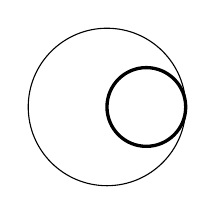
\begin{tikzpicture}[scale=.5]
\draw[very thick] (1,0) circle [radius=1];
\draw[scale=2] (0,0) circle [radius=1]; 
\end{tikzpicture}
\end{codeshow}
注意,组内的 \texttt{scale} 是正常图像的 \(0.5\times 2=1\) 倍.

使用负值来实现“翻转”效果,以及使用 \tikzkw{scale around} 来指定缩放中心:
\begin{tikzshow}[very thick]
\draw[thin] (0,0) circle [radius=1];
\draw[xscale=-1] (0,0) rectangle (1,1);
\draw[red, xscale=-1] (0,0) rectangle (1,1);
\draw[blue, scale around={1.5:(1,1)}] (0,0) rectangle (1,1);
\end{tikzshow}

\subsubsection{倾斜(slant)*}
倾斜不是一个常用的图像变换.\tikzz\ 中的倾斜指令是 \tikzkw{xslant} 与 \tikzkw{yslant}.简单地解释,\tikzkw{xslant} 会把图像中坐标为 \((x,y)\) 的点变换为 \((x+k\times y, y)\).
\begin{tikzshow}[very thick,scale=.6]
\draw[help lines] (0,0) grid (4,2);
\draw (0,0) -- (1,1) -- (1,2) -- cycle;
\draw[red, xslant=1.5] (0,0) -- (1,1) -- (1,2) -- cycle;
\draw[blue, xslant=-1] (0,0) -- (1,1) -- (1,2) -- cycle;
\end{tikzshow}

\subsection{裁剪(clip)}
在 \latexline{clip} 命令\RED{之后}的所有绘图都会只显示该裁剪视窗中的部分:
\begin{tikzshow}
\clip (0,0) rectangle (1.1, 1.1);
\draw[red, thick] (0,0) circle [radius=1];
\end{tikzshow}

添加 \tikzkw{draw} 选项可以把 \latexline{clip} 命令的“轮廓”绘制出来\footnote{也可使用 \latexline{draw} 命令并将 \tikzkw{clip} 作为参数,还可将两者作为 \latexline{path} 命令的参数.}:
\begin{tikzshow}
\clip[preaction={draw=red,ultra thick}] (1.2,0) arc [start angle=0, end angle=225, radius=1.2];
\draw (-1,-1) rectangle (1,1);
\draw (-1,1) -- (1,-1);
\end{tikzshow}
上例使用一个非闭合的路径(圆弧)来裁剪,\tikzz\ 会自动将其首尾连接.其中,\tikzkw{preaction} 选项表示在 \latexline{clip} 命令\RED{之前}先沿该路径按传递给其的参数绘制,之后再创建裁剪视窗;这样可以实现视窗样式的自定义(因为裁剪只影响其后的绘制命令).

\subsection{分组(scope)}
\label{subsec:scope}
分组操作允许你对当前组使用参数——这些参数会叠加到全局参数上,并且不影响到组外的对象:
\begin{codeshow}[listing outside text][3.5cm]
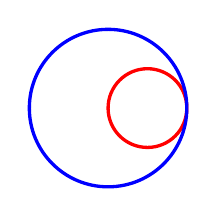
\begin{tikzpicture}[red, very thick, scale=.5]
\draw (1,0) circle [radius=1];
\begin{scope}[blue, scale=2]
\draw (0,0) circle [radius=1];
\end{scope}
\end{tikzpicture}
\end{codeshow}


\subsection{画布大小}
命令 \latexline{useasboundingbox} 可以

\section{点及其文本}
\subsection{点的绘制}
如果需要将点显式地绘制出来,使用 \latexline{node} 命令,或者 \latexline{draw} 命令的 \tikzkw{node} 选项.
\begin{tikzshow}
\node at (0,0) [circle, draw] {};
\node at (1,0) [circle, draw, fill=red] {};
\end{tikzshow}
花括号内可以添加文字内容,并使用 \tikzkw{anchor} 选项定义对齐方式;可传入的值是东西南北(east, west, south, north)以及 4 个复合方位(south west).或者你可以依次用 left, right, above, below 来替代:
\begin{tikzshow}
\draw[help lines] (0,0) grid (2,2);
\draw (0,0) node [anchor=south west] {$\beta$};
\node at (0,1) [above right] {Here};
\node at (1,0) [above=2pt] {Hi};
\draw (1,2) node [below right=1pt and 8pt] {$1,0$};
\end{tikzshow}
其中,如果要像最后一行一样给出两个距离参数,需加载 \tikzz\ 的 \pkg{positioning} 库.

\section{属性}
\label{sec:tikz-property}

\subsection{线宽}
\tikzz\ 预定义了 7 种线宽,从细到粗是:\tikzkw{ultra thin}, \tikzkw{very thin}, \tikzkw{thin}, \tikzkw{semithick}, \tikzkw{thick}, \tikzkw{very thick}, \tikzkw{ultra thick}.或者利用 \tikzkw{line width} 选项指定.
\begin{tikzshow}
\draw[ultra thin] (0,0) -- (1,0);
\draw[ultra thick] (1,0) -- (2,0);
\draw[line width=10pt] (0,1) -- (2,1);
\end{tikzshow}

\subsection{线型}
\tikzz\ 预定义了 4 种基本线型:\tikzkw{dashed}, \tikzkw{dotted}, \tikzkw{dash dot}, \tikzkw{dash dot dot}.它们还可以配合 \tikzkw{loosely} 或者 \tikzkw{densely} 进行微调.
\begin{tikzshow}
\draw[dashed] (0,0) -- (1,0);
\draw[dotted] (0,-0.5) -- (1,-0.5);
\draw[dash dot] (0,-1) -- (1,-1);
\draw[dash dot dot] (0,-1.5) -- (1,-1.5);
\draw[loosely dashed] (0,-2) -- (1,-2);
\draw[densely dotted] (0,-2.5) -- (1,-2.5);
\end{tikzshow}

如果的确需要深度自定义,请使用 \tikzkw{dash pattern} 自定义线型,并可配合 \tikzkw{dash phase} 指定线型的起始位置.
\begin{tikzshow}
\draw[dash pattern=on .1cm off .25cm on .25cm off .15cm, dash phase=1cm] (0,0) -- (3,0);
\end{tikzshow}

\subsection{箭头}
\tikzz\ 中的箭头多到可以单独开一个章节,但我并不想全部详尽地介绍.用大于或小于号表示箭头的指向,用竖线表示是否加上截断符号.一些基本的样例:
\begin{tikzshow}
\draw[->|] (1,3) -- (2,3);
\draw[stealth-] (1,2) -- (2,2);
\draw[->,>=stealth, line width=3pt] (1,1) arc [start angle=90, end angle=30, radius=1];
\draw[<->] (.5,4) -- (.5,0) -- (2.5,0);
\end{tikzshow}
其中,用 \texttt{>=stealth} 或 \texttt{-stealth} 的方式指定了箭头末端的类型为 \texttt{stealth}.你也可以将前者作为整个 \envi{tikzpicture} 环境的可选参数进行传递.

\tikzz\ 的 \pkg{arrows.meta} 库包含很多箭头,读者可以自行查阅.

\subsection{绘制颜色}
在绘制网格一节,已经使用过 \texttt{lightgray} 作为网格的绘制颜色;当时省略了 \tikzkw{draw} 选项.以下使用浅红色作为绘制色:
\begin{tikzshow}
\draw[draw=red!50!white, ultra thick] (0,0) rectangle (1,1);
\end{tikzshow}
其中,双感叹号加数字是表示插值比例为 0.5;\pkg{xcolor} 宏包支持该语法.

\subsection{单色填充}
填充命令 \latexline{fill} 只能使用于闭合区域,\textbf{且不绘制区域边界}.你可以在一般绘制命令的末尾添加 \tikzkw{cycle} 来创建一个闭合对象:
\begin{tikzshow}
\fill[green] (0,0) -- (1,0) -- (1,1) -- cycle;
\end{tikzshow}

在填充的同时绘制\footnote{准确地说,\latexline{filldraw} 命令是先绘制再填充.},使用 \latexline{filldraw} 命令,并分别指定绘制和填充颜色:
\begin{tikzshow}
\filldraw[draw=black, fill=cyan] (0,0) -- (2,0) arc (0:30:2);
\end{tikzshow}

利用区域的奇偶性填充,使用 \tikzkw{even odd rule}:
\begin{tikzshow}
\fill[even odd rule, blue] (0,0) -- (2,0.5) -- (1,1) circle (0.25);
\end{tikzshow}

\subsection{渐变填充*}
使用 \latexline{shade} 命令控制渐变填充,

\section{样式与高级控制}
\subsection{样式(style)}
如果某种属性需要用来反复作图,可以把它自定义为样式:

上文中出现过的 \texttt{help lines},就是 \tikzz\ 预定义的一种样式.

\subsection{循环语句}
\tikzz\ 支持循环语句,这一点对于科技绘图来说十分重要.
\begin{tikzshow}[place/.style={circle, draw, fill=black, minimum size=5pt, inner sep=0pt}]
\foreach \x in {1,2,3} {
    \node at (\x, 0) [place] {};
    \draw (\x, 0) circle [radius=1/\x];
}
\end{tikzshow}

有时候我们需要循环一个等差数列,这时候使用 \ldots 即可.\tikzz\ 会将 \(a,b,\ldots,c\) 识别为从 \(a\) 到 \(c\) 以 \(b-a\) 为公差的等差数列;如果你不指定 \(b\),那么默认以 \(1\) 为公差.
\begin{tikzshow}[place/.style={circle, draw, fill=black, minimum size=5pt, inner sep=0pt}]
\foreach \x in {1,1.5,...,3,4} {
    \node at (\x, 0) [place] {};
    \draw (\x, 0) circle [radius=\x/8];
}
\end{tikzshow}
上例中的 \(4\) 不在数列内,这样写是允许的.你也可以在数列后接着写另一个数列.

大部分需要知道“循环到列表第几个”的场合,都可以配合移动画笔或相对坐标命令实现:
\begin{tikzshow}[scale=.5]
\draw[red] (0,0) grid (3,3);
\foreach \x/\y in {0,1/2,2}
  \draw (\x, \y) +(.5,.5) circle [radius=.4];
\end{tikzshow}
上例同时循环了多个变量,中间用斜线分隔;它们分别按照列表中斜线分隔后的对应值进行循环.如果某一位置的列表值数量小于变量值,那么靠后的变量将都取最后一个值.

此外,如果 \latexline{foreach} 内部只有一条语句,像上例一样不添加花括号也是可以的.

\section{实用范例}
\label{sec:tikz-eg}
本节通过例子的方式,向读者展示 \tikzz\ 的常用情形.

% Appendices

% 参考文献
\bibliography{Bib}

% 附录
\clearpage
\appendix
% 重定义附录的chapter样式
\renewcommand{\chaformat}[1]{%
	\parbox[b]{.5\textwidth}{\raggedleft\bfseries \S 附录 \\ \vspace{0.2ex} #1} \quad\rule[-12pt]{2pt}{70pt}\quad
	{\fontsize{60}{60}\selectfont\thechapter}}

\chapter{注音符号}
\label{app:phonetic}
% 这里不用>{\ttfamily}而用\verb是为了减少报错可能
\begin{center}
\tabcaption{注音符号与特殊符号}
\begin{tabular}{|*{4}{>{\centering}p{3em} @{-\hspace{1em}} p{3em}|}}
\hline
\texttt{样式} & 命令 & \texttt{样式} & 命令 & \texttt{样式} & 命令 & \texttt{样式} & 命令 \\
\hline
\=o  & \verb|\=o|  & \'o  & \verb|\'o|  & \v o & \verb|\v o|  & \`o   & \verb|\`o|  \\
\^o  & \verb|\^o|  & \"o  & \verb|\"o|  & \.o  & \verb|\.o|   & \H o  & \verb|\H{o}| \\
\d o & \verb|\d{o}| & \u o & \verb|\u{o}| & \b o & \verb|\b{o}|  & \t oo & \verb|\t{oo}|\\
\multicolumn{2}{|c@{\bf --}}{$\tilde{o}$} & \multicolumn{2}{@{\bf --}c|}{\tt{\$$\backslash$tilde\{o\}\$}} &%
\multicolumn{2}{c@{\bf --}}{$\hat{o}$}    & \multicolumn{2}{@{\bf --}c|}{\tt{\$$\backslash$hat\{o\}\$}}\\
\multicolumn{8}{|c|}{} \\
\o  & \verb|\o|  & \O  & \verb|\O|  & \i  & \verb|\i|  & \j  & \verb|\j| \\
\aa & \verb|\aa| & \AA & \verb|\AA| & \ae & \verb|\ae| & \AE & \verb|\AE|\\
\oe & \verb|\oe| & \OE & \verb|\OE| & !`  & \verb|!`|  & ?`  & \verb|?`| \\
\hline
\end{tabular}
\end{center}

\mbox{}

\begin{center}
\tabcaption{国际音标输入表(部分)}
\begin{tabular}{|*{3}{>{\rmfamily}c !{-} >{\ttfamily}p{7.5em}|}}
\hline
\texttt{样式} & 命令 & \texttt{样式} & 命令 & \texttt{样式} & 命令 \\
\hline
\textdzlig & \char92textdzlig & \textesh & \char92textesh & \textteshlig & \char92textteshlig \\
\textdyoghlig & \char92textdyoghlig & \textturnv & \char92textturnv & \textschwa & \char92textschwa \\
\textscriptg & \char92textscriptg & \texttheta & \char92texttheta & \textupsilon & \char92textupsilon \\
\textscripta & \char92textscripta & \dh & \char92dh & \textepsilon & \char92textepsilon \\
\textopeno & \char92textopeno & \textyogh & \char92textyogh & \ng & \char92ng \\
\hline
\multicolumn{2}{|c|}{重音} & \multicolumn{2}{c|}{次重音} & \multicolumn{2}{c|}{长音节} \\
\textprimstress & \char92{}textprimstress & \textsecstress & \char92textsecstress & \textlengthmark & \char92textlengthmark \\
\hline
\end{tabular}
\end{center}

\textit{注:\texttt{\char92dh}命令在非CJK文档中有时编译会出现问题}。

\chapter{建议与其他}

除了参考文献列表中给出的书籍以外,我还推荐你用控制台在\TeX{} Live中能找到的以下书籍:

\medskip\begin{para}
\item[texdoc usrguide] \TeX\ Live自带的用户手册。
\item[texdoc clsguide] \TeX\ Live自带的文档类和宏包编写手册。
\item[texdoc fntguide] \TeX\ Live自带的字体使用手册。
\item[texdoc symbols-a4] 一份速查表,基本上所有的\LaTeX\ 字符命令都在这里了。
\item[texdoc latexcheat] 很有趣的命令表,只有两页。
\item[texdoc impatient] \emph{\TeX{} for the Impatient}, 一本介绍底层\TeX\ 的书。这也是我阅读的第一本\TeX\ 书,Knuth的\emph{The \TeX\ book}虽然血统正但是难啃啊。本书中译本在:\url{https://bitbucket.org/zohooo/impatient/wiki/Home}
\item[texdoc texbytopic] \emph{\TeX{} by Topic}, 个人觉得不如上面那本,但也许只是叙述方式不一样吧。
\end{para}
\bigskip

\noindent 你可能还需要的功能:
\begin{description}
\item[\pkg{mhchem}] 该宏包用于输入化学式,提供了\latexline{ce}命令。
\end{description}

% \tikzz\ 索引
%\setlength{\columnseprule}{0pt}
%\printindex

\end{document}
